\documentclass[a4paper,pdf]{article}
\usepackage{hyperref}
\usepackage{pdfpages} % http://mirror.unl.edu/ctan/macros/latex/contrib/pdfpages/pdfpages.pdf
\usepackage{booktabs} 
\usepackage[utf8]{inputenc}
\usepackage{sectsty}
\subsubsectionfont{\fontsize{12}{15}\selectfont}
\usepackage[dutch]{babel}
\usepackage[margin=1.4in]{geometry}
\usepackage{float}
\usepackage[justification=centering]{caption}
\usepackage[utf8]{inputenc}
\usepackage{amsmath}
\usepackage{mathtools}
\usepackage{graphicx}
\usepackage[colorinlistoftodos]{todonotes} % handig voor commentaar: gebruik \todo{}, zie ftp://ftp.fu-berlin.de/tex/CTAN/macros/latex/contrib/todonotes/todonotes.pdf
\usepackage{listings}
\usepackage{pdfpages}
\usepackage{tcolorbox}
\usepackage{float}
\usepackage[font={footnotesize}]{caption}
\usepackage{subcaption}
\usepackage{tabularx}
\usepackage{apacite}
\usepackage{enumitem}\usepackage{array}% http://ctan.org/pkg/array
\usepackage{lipsum}% http://ctan.org/pkg/lipsum
\usepackage{titlesec}
\usepackage{natbib}
\usepackage{hyperref}
\usepackage{xcolor}
\usepackage{ltxtable} 
\usepackage{longtable}
\usepackage{graphicx}
\usepackage{tikz}
\usepackage[nottoc,notlot,notlof]{tocbibind}
\usepackage{amsthm}
\usetikzlibrary{matrix}
\usetikzlibrary{tikzmark}
\selectlanguage{dutch}
%\tikzstyle{arrow} = [thick,->,>=stealth']

\newtheoremstyle{plain}
  {\topsep}   % ABOVESPACE
  {\topsep}   % BELOWSPACE
  {\itshape}  % BODYFONT
  {0pt}       % INDENT (empty value is the same as 0pt)
  {\bfseries} % HEADFONT
  {:}         % HEADPUNCT
  {5pt plus 1pt minus 1pt} % HEADSPACE
  {}          % CUSTOM-HEAD-SPEC


\newtheorem{theorem}{Stelling}
\newtheorem*{HOV}{Hoofdvraag}
\newtheorem{DV}{Deelvraag}
\newtheorem{SDV}{Subdeelvraag}[DV]

\usepackage{xcolor}
\hypersetup{
    colorlinks,
    linkcolor={black!42!black},
    citecolor={black!50!black},
    urlcolor={blue!50!black}
}

 
%\newcommand{\todo}[1]{\textbf{TODO: #1 }}
\begin{document}




%\makeatletter
%\renewcommand\paragraph{\@startsection{paragraph}{4}{\z@}%
%  {-3.25ex\@plus -1ex \@minus -.2ex}%
%  {1.5ex \@plus .2ex}%
%  {\normalfont\normalsize\bfseries}}
%\makeatother

%%% DIT IS DE TITLE PAGE VOOR INFORMATIEKUNDE NIET VOOR AI OF INFORMATICA! 
%% GEBRUIK VOOR AI OF INFORMATICA JE EIGEN TITLEPAGE TEMPLATES\


\begin{center}

\vspace{2.5cm}

% [CHANGE] The title of your thesis. If your thesis has a subtitle, then this
% should appear right below the main title, in a smaller font.
\begin{Huge}
Het Manipuleren van de Tweede Kamerverkiezingen door Uitbuiting van de Voorkeursdrempel
%Ondervertegenwoordigde Bevolkingsgroepen Adequater Vertegenwoordigd in de Tweede Kamer
\end{Huge}

\vspace{1.5cm}

% [CHANGE] Your full name. In case of multiple names, you can include their
% initials as well, e.g. "Jan G.J. van der Wegge".
\emph{Auteur}\\
Micha\"{e}l Amir\\
% [CHANGE] Your student ID, as this has been assigned to you by the UvA
% administration.
10580247

\vspace{0.5cm}

% [DO NOT CHANGE]
Bachelor Scriptie\\
% [CHANGE] Whether your Bachelor thesis is 6 ECTS (regular) or 9 ECTS (Honours
% programme).
Credits: 12 EC

\vspace{0.5cm}

% [DO NOT CHANGE] The name of the educational programme.
Bachelor Opleiding Informatiekunde

\vspace{0.25cm}

% [DO NOT CHANGE] The addess of the educational programme.
Universiteit van Amsterdam\\
Faculteit der Natuurwetenschappen, Wiskunde en Informatica\\
Science Park 904\\
1098 XH Amsterdam

\vspace{1cm}
\begin{figure}[H]
\centering

	
\includegraphics[width=0.1\linewidth]{UVA.png}

\end{figure}


\vspace{1cm}

\emph{Begeleider \& Eerste Examinator}\\
% [CHANGE] The name of your supervisor. Include the titles of your supervisor,
% as well as the initials for *all* of his/her first names.
Dr. M. J. Marx

\vspace{0.25cm}

% [CHANGE] The address of the institute at which your supervisor is working.
% Be sure to include (1) institute (is appropriate), (2) faculty (if
% appropriate), (3) organisation name, (4) organisation address (2 lines).
ILPS, IvI\\
Faculteit der Natuurwetenschappen, Wiskunde en Informatica\\
Universiteit van Amsterdam\\
Science Park 904\\
1098 XH  Amsterdam

\vspace{1cm}

\emph{Tweede Examinator}\\
% [CHANGE] The name of your supervisor. Include the titles of your supervisor,
% as well as the initials for *all* of his/her first names.
Dr. J. A. C. Sandberg

\vspace{0.25cm}
IvI\\
Faculteit der Natuurwetenschappen, Wiskunde en Informatica\\
Universiteit van Amsterdam\\
Science Park 904\\
1098 XH  Amsterdam
\vspace{1cm}

% [CHANGE] The date at which you will finalize and submit your thesis.
20-06-2016
\thispagestyle{empty}

\end{center}



\pagebreak

\tableofcontents


\pagebreak

\begin{abstract}
Bepaalde bevolkingsgroepen zijn in de Nederlandse Tweede Kamer ondervertegenwoordigd. Daarnaast ontbreekt ook elke vorm van een quotum zij zowel de politieke partijen als de Tweede Kamer als geheel. Daarom zijn er in dit onderzoek een vijftal strategie\"{e}n ontwikkeld die de ondervertegenwoordigde bevolkingsgroepen in staat stellen om de regel van de voorkeursdrempel in de kieswet beter te benutten om zo adequater vertegenwoordigd te zijn. Vanwege de complexiteit van de wijze waarop een strategie uitgevoerd dient te worden, worden een tweetal hulpmiddelen in de vorm van IT-toepassingen voorgesteld. Tot slot wordt er onderzocht wat er gebeurt wanneer meerdere bevolkingsgroepen een strategie uitvoeren. Hierbij wordt met \textit{P=percentage stemmen afkomstig uit een bevolkingsgroep in verhouding tot totaal aantal stemmen} en \textit{Z=aantal zetels} een Nash Equilibrium bereikt wanneer geldt: \textit{P*Z/(1-P)*Z}. Om te voorkomen dat een bevolkingsgroep oververtegenwoordigd zal zijn nadat het een strategie heeft uitgevoerd, wordt gesteld dat dit voorkomen kan worden door de voorkeursdrempel verhogen naar het aantal stemmen dat geldt voor de kiesdeler. 

\iffalse
Bevolkingsgroepen kunnen dan in geen geval een groter aandeel van de zetels ontvangen dan dat het aantal stemmen dat zij hebben ontvangen in verhouding tot het totaal aantal stemmen. Oftewel, bij volle 100\%  deelname van leden van een bevolkingsgroep ontvangt deze bevolkingsgroep een even groot aandeel van de zetels als het aandeel van de stemmen dat is uitgebracht.  
\fi


\end{abstract}


\pagebreak

\hypersetup{
    colorlinks,
    linkcolor={blue!50!black},
    citecolor={black!50!black},
    urlcolor={blue!37!black}
}


% Here you input all your sections in seperate files

\section{Introductie}
\label{sec:intro}
Bij de Tweede Kamerverkiezingen in Nederland kunnen kandidaten met voorkeurstemmen gekozen worden. Hierbij moet een kandidaat een kwart van het aantal stemmen halen dat een partij nodig heeft om één zetel te behalen. Het aantal stemmen dat behaald moet worden voor één zetel wordt de \textit{kiesdeler} genoemd. Het aantal stemmen dat een kandidaat nodig heeft om met voorkeur gekozen te worden wordt de \textit{voorkeursdrempel} genoemd. De voorkeursdrempel is een kwart van de kiesdeler  \citep{Kiesraad_voorkeursdrempel2}.  In de historie van de Tweede Kamerverkiezingen in Nederland is het slechts twaalf maal voorgekomen dat een kandidaat met voorkeurstemmen in de Tweede Kamer is gekozen \citep{Voork74:online}. Bij de Tweede Kamerverkiezingen van 2012 is dit voor het laatst gebeurt. Pieter Omtzigt van het CDA werd toen met voorkeurstemmen gekozen.\

Dit onderzoek is grotendeels gemodelleerd op de Tweede Kamerverkiezingen van 2012. Bij deze verkiezingen werd er voornamelijk op de hoogst genoteerde kandidaten gestemd (zie Figuur \ref{fig:sv2012}). Lager genoteerde kandidaten ontvingen over het algemeen niet genoeg stemmen om boven de voorkeursdrempel uit te komen. Hierdoor zijn, op Pieter Omtzigt na, alle kandidaten op basis van hun plaats op de kandidatenlijst in de Tweede Kamer gekozen. Bij het verdelen van de zetels aan de kandidaten wordt er, conform de kieswet \citeyearpar{kieswetje}, eerst gekeken naar het aantal stemmen die een kandidaat heeft ontvangen. Vervolgens wordt er pas gekeken naar de plaats op de kandidatenlijst. Een kandidaat die aan de voorkeursdrempel voldoet krijgt zodoende de voorkeur boven een kandidaat die hoger genoteerd staat maar niet aan de voorkeursdrempel voldoet. 


\begin{figure}[H]


	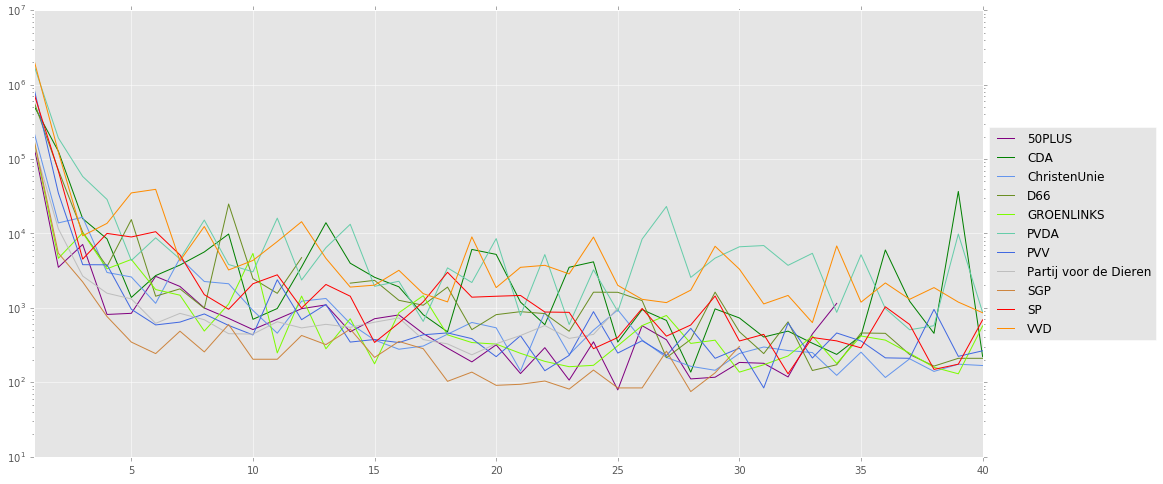
\includegraphics[width=\linewidth]{verdeling_stemmen_2012.png}

			\caption{Per partij de verdeling van de stemmen over de eerste veertig kandidaten bij de Tweede Kamerverkiezingen van 2012. Ten behoeve van de leesbaarheid is er een logaritme over de y-as toegepast.}

\label{fig:sv2012}
\end{figure}

In dit onderzoek zullen we gaan kijken hoe specifieke bevolkingsgroepen de regel van de voorkeursdrempel in hun voordeel kunnen gebruiken om in hogere mate vertegenwoordigd te worden. Deze bevolkingsgroepen zijn:\\

\newcolumntype{L}{@{}>{\bfseries}p{16em}<{}}% Item label
\newcolumntype{I}{X@{}}% Item contents
\noindent\begin{tabularx}{\textwidth}{LI}
Vrouwen: & De stemgerechtigde vrouwen in Nederland. \\
  \\
 Allochtonen: & De stemgerechtigde allochtonen in Nederland. Hierbij wordt de definitie van het CBS  \citeyearpar{Watve22:online} gehanteerd. Volgens het CBS is een persoon een allochtoon wanneer de persoon zelf of één van de ouders van de persoon in het buitenland is geboren. We maken hierbij geen onderscheid tussen westerse en niet-westerse allochtonen.
\\
\end{tabularx}
  
  \newcolumntype{L}{@{}>{\bfseries}p{16em}<{}}% Item label
\newcolumntype{I}{X@{}}% Item contents
\noindent\begin{tabularx}{\textwidth}{LI}

  Ouderen: & De stemgerechtigden personen met een leeftijd van vijftig jaar en ouder. Hierbij worden de definities van de Rijksoverheid \citeyearpar{Wiebe32:online} gecombineerd. Volgens de Rijksoverheid is er geen strike definitie van een oudere. De Rijksoverheid definieert oudere op de arbeidsmarkt als personen van vijftig tot 65 jaar. Bij AOW-gerechtigden gaat het om personen van 65 jaar en ouder. Zodoende combineren we deze twee definities tot één definitie.  \\
\\  
Provincialen: & Voor de provincialen is er geen allesomvattende definitie te vinden. Zodoende hebben we de definitie Randstedelingen gebruikt om personen wonenden in de Randstad te defini\"{e}ren \citep{Rands36:online}. Stemgerechtigde personen niet in de Randstad wonen worden in dit onderzoek aangeduid met provincialen. \\
  \\
\end{tabularx}

In Figuur \ref{fig:az2012} zien we in welke aantallen de bovenstaande bevolkingsgroepen vertegenwoordigd zijn. Aan de hand van data verkregen van het CBS \citeyearpar{CBS_stemgedrag} is onderzocht of de vertegenwoordiging van de bevolkingsgroepen een afspiegeling is van de stemgerechtigden in Nederland ten tijde van de Tweede Kamer verkiezingen in 2012.
De verdeling van het aantal stemgerechtigde vrouwen en mannen in Nederland in 2012 was nagenoeg gelijk met beiden een 50\% aandeel in het aantal stemgerechtigden. Zodoende kunnen we concluderen dat de bevolkingsgroep vrouwen ondervertegenwoordigd is met een aandeel van 38,7\% van de zetels. 
De verdeling stemgerechtigde allochtonen en autochtonen in Nederland in 2012 was grofweg 20\% allochtonen om 80\% autochtonen. Zodoende kunnen we concluderen dat ook de bevolkingsgroep allochtonen ondervertegenwoordigd is met een aandeel van 8,7\% van de zetels. 
De verdeling van het aantal stemgerechtigde ouderen en het aantal stemgerechtigden met een leeftijd van onder de vijftig jaar in Nederland in 2012 was grofweg 49\% ouderen en 51\% stemgerechtigden met een leeftijd van onder de vijftig jaar. Zodoende kunnen we ook voor de bevolkingsgroep ouderen concluderen dat zij met 25.3\% van de zetels ondervertegenwoordigd zijn in de Tweede Kamer. 
De verdeling van het aantal stemgerechtigde provincialen en Randstedelingen was grofweg 67\% provincialen om 33\% Randstedelingen. Zodoende kunnen we ook voor de bevolkingsgroep provincialen concluderen dat zij met 50\% van de zetels ondervertegenwoordigd zijn in de Tweede Kamer. 

\begin{figure}[H]
\centering

	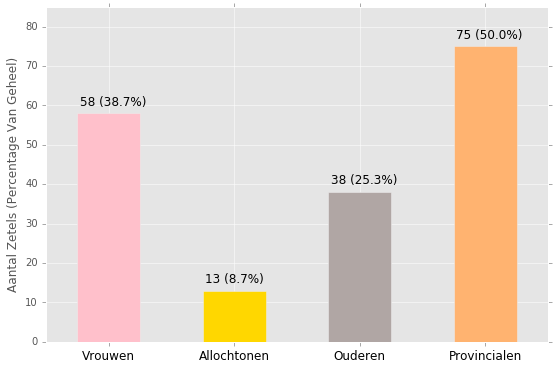
\includegraphics[width=0.55\linewidth]{aantal_zetels_bevolkingsgroepen.png}

			\caption{Het aantal gekozen kamerleden per bevolkingsgroep bij de Tweede Kamerverkiezingen van 2012. De groepen zijn allen van een eigen kleur voorzien. Deze kleuren zullen in het gehele paper corresponderen met de bevolkingsgroepen.}

\label{fig:az2012}
\end{figure}

Naast het feit dat de beschreven bevolkingsgroepen ondervertegenwoordigd zijn in de Tweede Kamer na de verkiezingsuitslag van 2012, is uit diverse literatuur op te maken dat het voor de bevolkingsgroepen alsmede voor de politiek en de democratie gunstig is wanneer een parlement aan afspiegeling van de samenleving  \citep{tremblay1998female,anwar2001participation}. Uit een onderzoek van \cite{banducci2004minority} blijkt dat des te beter bevolkingsgroepen als vrouwen en minderheden vertegenwoordigd worden in het parlement, des te positiever er vanuit deze bevolkingsgroepen tegen de politiek aangekeken wordt. Tevens wordt onder deze bevolkingsgroepen de deelname aan parlementsverkiezingen vergroot. Onderzoek van \cite{wangnerud2009women} en \cite{sainsbury2004women} toont aan dat de belangen van vrouwen steeds beter behartigd worden naarmate het aantal vrouwelijke leden in het parlement toeneemt. Volgens \cite{mansbridge1999should} worden vrouwen en negeroïde burgers het beste vertegenwoordigd door respectievelijk vrouwelijk en negeroïde parlementsleden. De reden hiervoor is dat deze parlementsleden bedachtzamer kunnen opereren wanneer het om politieke kwesties gaat die deze leden van de bevolking treffen. Uit een onderzoek van \cite{broockman2014female} blijkt, in tegenstelling tot de verwachting, dat een stijging in het aantal vrouwen dat een politiek ambt bekleedt er niet toe leidt dat er meer vrouwen naar de stembus gaan. Echter heeft het onderzoek enkel betrekking op de Verenigde Staten en wordt geen verder onderzoek verricht naar de toe- of afname van de algehele betrokkenheid van vrouwen voor de politiek en de politieke besluitvorming. In het onderzoek van \cite{karp2008politics} wordt er echter wel geconcludeerd dat betrokkenheid onder vrouwen voor de politiek toeneemt naar mate meer vrouwen zich kandideren voor verkiezingen en naar mate er meer vrouwen een politieke ambt bekleden. 

Naast de effecten die adequatere vertegenwoordiging van bepaalde bevolkingsgroepen met zich meebrengen, blijk dat vrouwen en minderheden beter vertegenwoordigd zijn in landen waar een evenredige vertegenwoordiging wordt gehanteerd \citep{macivor1999proportional,mcallister2002electoral,studlar1999will,welch1990multi}.  Nederland is een land dat een evenredige vertegenwoordiging hanteert. Dit houdt in dat het percentage stemmen evenredig is met het percentage te ontvangen zetels \citep{Kiess35:online}. Oftewel als een partij 10\% van de stemmen heeft ontvangen krijgt deze partij ook 10\% van de zetels.

Al het voorgaande in ogenschouw nemend wordt er in dit onderzoek onderzocht of er strategie\"{e}n op te stellen zijn onder de leden van de verschillende bevolkingsgroepen waardoor zij adequater vertegenwoordigd kunnen worden in de Tweede Kamer. Binnen dit onderzoek gaan we uit van de meest realistische aannames. Dit houdt in dat we uitgaan van de verdeling van zetels en stemmen over de partijen zoals deze werden voorspeld bij de laatste peiling van 11 september 2012 \citep{IPSOS} en zoals deze daadwerkelijk waren na de verkiezingsuitslag van 2012 \citep{Kiesraad_uitslag}. Aan de hand van de peilingen proberen we strategie\"{e}n op te zetten en aan de hand van de einduitslag zullen we testen hoe succesvol deze strategie\"{e}n zouden zijn geweest. Het doel is om met behulp van deze strategie\"{e}n een maximum aantal leden van een bevolkingsgroep in de Tweede Kamer te krijgen door effectiever gebruikt te maken van de voorkeursdrempel. De hoofdonderzoeksvraag luidt dan ook: \\


\begin{HOV}
\large
"Hoe kunnen specifieke bevolkingsgroepen in Nederland bij de Tweede Kamerverkiezingen de regel van de voorkeursdrempel in de kieswet gebruiken in hun voordeel?"\\
\end{HOV}

\normalsize
Om tot een antwoord op de bovenstaande hoofdonderzoeksvraag te komen zullen we met het onderzoek verder de diepte in gaan d.m.v. opdeling in deelvragen. Hiervoor hebben zijn vijf deelvragen opgezet en twee subdeelvragen. Aan de hand van de eerste deelvraag zullen we onderzoeken wat het maximum aantal kandidaten per bevolkingsgroep zou zijn geweest wanneer de bevolkingsgroep bepaalde strategie\"{e}n hadden uitgevoerd. De eerste deelvraag luidt daarmee als volgt:\\

\begin{DV}
"Wat is het theoretisch maximum aantal kandidaten dat per specifieke bevolkingsgroep gekozen kan worden in de Tweede Kamer?"\\\
\end{DV}

Deze eerste deelvraag zal worden beantwoord in Hoofdstuk \ref{sec:eva}. In dit hoofdstuk zullen we vijf verschillende soorten strategie\"{e}n gaan uitrollen en per  bevolkingsgroep gaan toepassen. Aan de hand van de peilingen proberen we eerst een voorspelling te doen hoe de stemmen verdeeld zullen worden wanneer 100\% van de bevolkingsgroep zich committeert aan een strategie. Vervolgens zullen we in het daaropvolgende hoofdstuk gaan onderzoeken welke factoren er van invloed kunnen zijn op het behalen van het maximum aantal kandidaten per bevolkingsgroep. De tweede deelvraag luidt daarom: \\

\begin{DV}" Welke factoren kunnen per bevolkingsgroep van invloed zijn op het wel of niet behalen van het theoretisch maximum aantal kandidaten dat in de Tweede Kamer gekozen kan worden?"\\\
\end{DV}

Nadat de factoren en hun invloed zijn beschreven, wordt er onderzocht welke strate\"{e}n aan te bevelen zijn richting de bevolkingsgroepen. De derde deelvraag luidt:\\

\begin{DV}"Welke strategie is per specifieke bevolkingsgroep aan te bevelen wanneer zij de regel van de voorkeursdrempel in de kieswet willen benutten in hun voordeel?"\\\
\end{DV}

Vanwege de verleiding te kiezen voor een strategie die in Hoofdstuk \ref{sec:eva} zich bewezen heeft als de strategie met het hoogste rendement kan men geneigd zijn de complexiteit van een strategie over het hoofd te zien als het gaat om de wijze van uitvoering. Vandaar dat dit onderzoek bij deze deelvraag niet poogt om een direct antwoord te hierop te verschaffen maar zal er verder de diepte ingegaan worden om daarmee te onderzoeken hoe de strategie\"{e}n uit te voeren zijn. Derhalve wordt de derde deelvraag verder opgedeeld in twee subdeelvragen. De eerste subdeelvraag luidt:\\

\begin{SDV}"Hoe kan een strategie uitvoerbaar worden gemaakt voor een specifieke bevolkingsgroep waarvan de leden zich willen committeren aan een strategie om de regel van de voorkeursdrempel in hun voordeel te benutten?"\\\
\end{SDV}

Met het beantwoorden van deze subdeelvraag zullen we een tweetal van hulpmiddelen voorstellen in de vorm van IT-toepassingen. Tevens stellen we ook een derde hulpmiddel voor. Dit derde hulpmiddel is een mengvorm van de eerste twee hulpmiddelen. Deze hulpmiddelen zullen slechts dienen als voorbeelden en verder onderzoek zal hierbij ook nodig zijn wanneer deze toepassingen daadwerkelijk worden ontwikkeld. Echter zullen we al wel ingaan op enkel voor- en nadelen die deze hulpmiddelen met zich mee kunnen brengen. Tevens zullen we de voor- en nadelen onderzoeken die kunnen ontstaan wanneer er geen hulpmiddelen worden ingeschakeld. Zodoende luidt de tweede subdeelvraag als volgt: \\\

\begin{SDV}"Wat zijn de eventuele voor- en nadelen van de keuze van de wijze waarop een strategie zal worden uitgevoerd?"\\\
\end{SDV}

Nadat a.d.h.v. de eerste deelvraag is onderzocht met welke strategie\"{e}n het maximum aantal vertegenwoordigers van een bevolkingsgroep in de Tweede Kamer gekozen hadden kunnen worden, wordt in Hoofdstuk \ref{h7} onderzocht wat er kan gebeuren wanneer leden van een andere bevolkingsgroep (of bevolkingsgroepen) zich committeert aan een tegenstrategie. Hierbij zullen we onderzoeken of er een toestand bereikt kan worden waarin beiden (of meerdere) bevolkingsgroepen een strategie hanteren en er een Nash Equilibrium onstaat. Hierbij luidt de vierde deelvraag: \\\

\begin{DV}"Wat kan er gebeuren wanneer een bevolkingsgroep zich committeert aan een strategie en een andere bevolkingsgroep zich committeert aan een tegenstrategie?"\\\
\end{DV}

Tot slot zal er een advies worden uitgebracht betreffende het voorkomen van uitbuiting van de voorkeursdrempel. Hierbij kunnen twee (of meerdere) bevolkingsgroepen een strategie uitvoeren maar geen van beide bevolkingsgroepen kan daarbij de regel van de voorkeursdrempel in haar/zijn eigen voordeel op zo een manier weten uit te buiten dat het d.m.v. het uitvoeren van een strategie oververtegenwoordigd zal zijn. Oftewel we adviseren een aanpassing van de kieswet wat er voor moet zorgen dat er geen overmatig misbruik van de regel van de voorkeursdrempel mogelijk zal zijn. De laatste deelvraag luidt daarom: \\\

\begin{DV}" Hoe kan er voorkomen worden dat de voorkeursdrempel niet in het voordeel van een bevolkingsgroep kan worden uitgebuit?"\\\
\end{DV}

Nadat de deelvragen zo adequaat mogelijk zijn beantwoord, zal er een conclusie getrokken worden en een aantal aanbevelingen gedaan worden op basis van bevindingen in het onderzoek. 






\iffalse
\begin{itemize}
\item Bevat je onderzoeksvraag (of vragen)
\item Plaatst je vraag in de bestaande literatuur.
\end{itemize}

Je onderzoeksvraag is leidend voor je hele scriptie. Alles wat je doet moet uiteindelijk terug te voeren zijn op 1 doel: het beantwoorden van die vraag. 

Typisch zal je het dan ook zo doen:

Mijn onderzoeksvraag is onderverdeeld in de volgende deelvragen:

\begin{description}
\item[RQ1] \ldots We   beantwoorden deze vraag  door het volgende te doen/ antwoord op de volgende vragen te vinden/ \ldots
\begin{enumerate}
\item Vragen op dit niveau kan je echt beantwoorden, en dat doe je in je Evaluatie sectie~\ref{sec:eva}.
\end{enumerate}
\item[RQ2] \ldots
\item[RQ3] \ldots
\end{description}

Je Evaluatie sectie~\ref{sec:eva} bevat evenveel subsecties als je deelvragen hebt. En in elke sectie beantwoord je dan die deelvraag met behulp van de vragen op het onderste niveau.

In je conclusies kan je dan je hoofdvraag gaan beantwoorden op basis van al het eerder vergaarde bewijs.


\paragraph{Overview of thesis}
Hier geef je even kort weer wat in elke sectie staat.
\fi



\newpage
\section{Gerelateerd Werk}
\label{sec:rel}
Zoals in de introductie al is genoemd, hanteert Nederland een evenredig kiesstelsel en draagt dit kiesstelsel positief bij aan de vertegenwoordiging van vrouwen en minderheden. In 2005 stelde toenmalig minister De Graaf van Bestuurlijke Vernieuwing voor het kiesstelsel om te gooien en een tweestemmenstelsel te combineren met een stelsel van meervoudige kiesdistricten. Hierbij zouden de kiezers zowel op een lokale kandidaat stemmen alsmede een landelijke kandidaat. In het onderzoek van \cite{norris2006impact} is berekend dat het voorstel van minister De Graaf een negatieve invloed zou hebben op het aantal vrouwelijke kamerleden. Gelukkig voor de vrouwen in Nederland is het voorstel van de minister verworpen. Desalniettemin is Nederland een land wat relatief weinig maatregelen heeft genomen als het gaat om het adequater vertegenwoordigen van vrouwen en tevens ook van minderheden. Daarentegen zijn er met name in de laatste twintig á dertig jaar zijn er wereldwijd steeds meer maatregelen in het leven geroepen die ervoor hebben moeten zorgen dat vrouwen en minderheden adequater vertegenwoordigd zouden worden in volksvertegenwoordigingen \citep{norris2007opening}. Een van de maatregelen die in het leven is geroepen in een quotum. De quota hebben wereldwijd hoofdzakelijk drie soorten vormen. Hier gaan we in dit hoofdstuk in de eerstvolgende sectie dieper op in.

Naast dat we dieper ingaan op de maatregelen die genomen kunnen worden om vrouwen en minderheden adequater te vertegenwoordigen, zullen we ook kijken naar IT-toepassingen en het effect daarvan op het vergroten van de betrokkenheid en participatie van stemgerechtigden en andere burgers. In Hoofdstuk \ref{h6} zullen we een tweetal IT-toepassingen presenteren die moeten bijdragen aan de in dit onderzoek ontwikkelde strate\"{e}n zoals wordt beschreven in Hoofdstuk \ref{sec:eva}. In het huidige hoofdstuk zullen derhalve ook dieper ingaan op enkele vormen van IT-toepassingen die al zijn ontwikkeld voor Tweede Kamerverkiezingen in Nederland. 

\subsection{Quota.} 
Wereldwijd zijn er drie soorten quota te onderscheiden die eraan bijdragen dat vrouwen en minderheden adequater vertegenwoordigd worden in volksvertegenwoordigingen. Deze quota zijn:  gereserveerde zetels, wettelijk vastgelegde quota en vrijwillige quota \citep{norris2007opening}. 

Gereserveerde zetels zijn zetels die specifiek voor leden van een bepaalde bevolkingsgroep zijn vastgesteld. De partijen die deze zetels ontvangen moeten deze zetels opvullen met een kandidaat afkomstig uit de bevolkingsgroep waarvoor deze bedoeld is. In sommige landen is het zo dat wanneer dit niet gebeurt de zetel wordt vergeven aan een andere partij die wel aan de wet regel kan voldoen. Het quotum-systeem van de gereserveerde zetel wordt met name toegepast in jonge (transitionele) democrati\"{e}n. Bij een wettelijk vastgelegde quotum is het zo bijvoorbeeld zo dat er in de wet staat hoeveel procent van de verkiezingskandidaten van een partij vanuit een bepaalde bevolkingsgroep afkomstig moet zijn. In Europa hanteren bijvoorbeeld Belgi\"{e}, Frankrijk en Spanje een dergelijke quotum
 \citep{council2012positive}. Bij een vrijwillige quotum tot slot, is de partij vrij om zelf te bepalen of zij een quotum invoeren of niet. Er is niets in de wet vastgelegd dat partijen een quotum moeten hanteren. Nederland is een land waar een vrijwillig quotum bestaat. De meeste partijen hadden een redelijk aantal vrouwelijke kandidaten op de kandidatenlijsten hadden staan bij de verkiezingen van 2012. Echter had de SGP geen enkele vrouwelijke kandidaat op de kandidatenlijst staan. De reden hiervoor ligt ten grondslag aan religieuze overtuigingen die er binnen de partij heersen. Echter moet de SGP van het Europese Hof van de Rechten van de Mens bij de eerstvolgende verkiezingen ook vrouwelijke kandidaten opnemen op de kandidatenlijst \citep{Nudef30:online}. Wat betreft de bevolkingsgroep allochtonen zijn er zelfs twee partijen die geen allochtone kandidaten op de kandidatenlijst hebben. Dit zijn de Partij voor de Dieren en (nogmaals) de SGP. Andere West-Europese landen die een vrijwillig quotum-systeem hanteren zijn Duitsland, Zwitserland en Groot Brittannië \citep{Quota47:online}. Een onderzoek van \cite{ryan2010politics} wijst uit dat in Groot Brittannië de partijen in veel gevallen een eigen quotum hanteren als het gaat om het aantal vrouwen op de kandidatenlijsten voor verschillende verkiezingen. Tevens blijkt uit dit onderzoek dat de vrouwelijke kandidaten vooral door deze partijen naar voren worden geschoven in districten (Groot Brittannië hanteert een districtenstelsel) waar de partij een kleine kans maakt om te winnen. 

Zoals hierboven al genoemd is ook Nederland een land waar een vrijwillig quotum-systeem wordt gehanteerd.  Doch hanteert geen enkele partij een quotum als het gaat om het aantal kandidaten afkomstig uit één van de in dit onderzoek beschreven bevolkingsgroepen. Sterker nog, de SGP wil geen vrouwelijke kandidaten op de kandidatenlijst. Het ontbreken van een quotum bij de Nederlandse politieke partijen geeft des te meer redenen voor leden van de vier bevolkingsgroepen om zich te committeren aan een strategie waardoor zij adequater vertegenwoordigd kunnen worden in de Tweede Kamer.

\subsection{IT-toepassingen bij verkiezingen.}
Verder in dit onderzoek stellen we een tweetal IT-toepassingen voor die leden van de bevolkingsgroep kunnen helpen bij het uitvoeren van een strategie (zie Hoofdstuk \ref{h6}). In Nederland zijn er de laatste jaren een aantal IT-toepassingen ontwikkeld om die dienen ter ondersteuning van de kiezers. Zo wordt de \textit{StemWijzer} al sinds de Tweede Kamerverkiezingen van 1998 in een online vorm gebruikt door vele kiezers \citep{kleinnijenhuis2007nederland}. Bij de StemWijzer worden de kiezers enkele stellingen voorgelegd. De kiezer kan aangeven in hoeverre zij/hij het met de stelling eens is. Aan de hand van de mening van de kiezer wordt vervolgens een advies gegeven over welke partij het beste bij de opinie van de kiezer past. Een vergelijkbare toepassing is het \textit{Kieskompas}. De werking van het Kieskompas is vrijwel hetzelfde als die van de StemWijzer. Echter stellen \cite{kleinnijenhuis2007nederland} in hun onderzoek dat bij de Tweede Kamerverkiezingen van 2006 de SP een voordeel had tegenover andere partijen. De VVD en de PVDA waren in het nadeel in vergelijking met andere partijen. Bij het Kieskompas waren vooral de kleine rechtse partijen in het voordeel en de VVD ook hierbij in het nadeel in vergelijking met andere partijen. Tevens stellen zij niet alle factoren in beschwouing worden genomen in het geven van een advies door zowel de StemWijzer als het Kieskompas. Zodoende komt het voor dat sommige kiezers een incorrect stemadvies krijgen. Uit onderzoek van \cite{garzia2012voting} blijkt dat 38\% van de stemgerechtigden de StemWijzer of het Kieskompas hebben gebruikt om tot hun stem te komen. Ook blijkt uit hun onderzoek dat er soortgelijke toepassingen zijn in andere Europese landen zoals bijvoorbeeld Duitsland, Belgi\"{e} en Groot Brittani\"{e}. Naast de StemWijzer en het Kieskompas bestaan er in Nederland ook soortgelijke online toepassingen voor specifieke bevolkingsgroepen. Zo is een een stemwijzer voor een stemwijzer voor jongeren \citep{Jonge36:online}, was er bij de Tweede Kamerverkiezingen van 2012 een stemwijzer voor ouderen \citep{Stemw79:online,Stemw68:online} en is er zelfs een stemwijzer voor cannabisgebruikers \citep{Canna56:online}.

Naast de toepassingen die dienen als hulpmiddel bij het maken van een partijkeuze is er ook een mobiele applicatie die ervoor moet zorgen dat er meer jongeren naar de stembus gaan \citep{Verki80:online}. Deze mobiele applicatie, de \textit{Verkiezingsapp} genoemd, poogt jongeren op een moderne manier enthousiast te maken voor verkiezingen. In de mobiele applicaties komen thema's naar voren waar jongeren mee te maken krijgen. Tevens zijn de gebruikers in staat hun eigen meningen en bevindingen te delen met andere jongeren via \textit{social media}. Enig onderzoek van wetenschappelijk aard ontbreekt echter als het gaat om het effect van de Verkiezingsapp. 

In de literatuur wordt er een positief effect beschreven als het gaat om IT-toepassingen en het vergroten van betrokkenheid en participatie van stemgerechtigden en andere burgers tijdens verkiezing en tevens voor het democratische politieke proces als geheel \citep{drezner2008power,doostdar2004vulgar,gimmler2001deliberative}. Ook al zullen de toepassingen niet altijd 100\% perfect zijn, blijkt het wel zo te zijn dat mensen zich goed geïnformeerd achten wanneer zij dit soort middelen aanwenden. Zo worden in Nederland zowel de StemWijzer als het Kieskompas als een positieve aanvulling op bestaande middelen ervaren. \citep{van2013kieskompas}.










\iffalse
Deze sectie bestaat uit een aantal "blokken", waarin je per blok de relevante literatuur beschrijft. 

Neem alleen literatuur op die van belang is voor jouw onderzoeksvraag en deelvragen.

Typisch heb je 1 blok voor je hoofdvraag en per deelvraag \textbf{RQi} een blok. 


\subsection{RQ1}

\subsection{RQ2}
\fi
\newpage
\section{Beschrijving van de Data.}
\label{sec:meth}

De data betreffende de Tweede Kamerverkiezingen van 2012 is een verzameling van open databestanden en databestanden verkregen van onderzoeksbureau IPSOS Nederland \citeyearpar{IPSOS}.
Ten doeleinde van dit onderzoek zijn verschillende dataset met elkaar gecombineerd om zodoende te pogen antwoorden te krijgen op de voor dit onderzoek opgestelde onderzoeksvragen. Met name voor de onderzoeksvraag betreffende het theoretisch maximum van vertegenwoordiging van bepaalde Nederlandse bevolkingsgroepen, is er data verzameld en zijn datasets met elkaar gecombineerd. De bevolkingsgroepen zijn: vrouwen, allochtonen, ouderen (met stemrecht en een leeftijd van 50 jaar en ouder) en provincialen (personen met stemrecht die buiten de Randstad-gemeenten wonen). Naast dataset die specifiek betrekking hebben tot één van de bevolkingsgroepen, zijn er ook algemene dataset gebruikt die op vrijwel alle bevolkingsgroepen van toepassing zijn. Allereerst volgt een beschrijving van de algemene datasets. Vervolgens worden per bevolkingsgroep de datasets beschreven.

\subsection*{Algemene Datasets.}
Wat de algemene data betreft gaat het hier om data die niet specifiek op één bevolkingsgroep betrekking had maar op meerdere bevolkingsgroepen. Deze dataset zijn: \\


\newcolumntype{L}{@{}>{\bfseries}p{13em}<{}}% Item label
\newcolumntype{I}{X@{}}% Item contents
\noindent\begin{tabularx}{\textwidth}{LI}
Landelijke peiling:  & Landelijke peiling aan de vooravond van de verkiezingen \citep{IPSOS}. In Figuur \ref{fig:pzL} is een grafiek te zien met de zetelverdeling  op basis van de peiling (lichtgekleurde staven). \\
  \\
Kandidatenlijsten: & De kandidatenlijsten van de partijen die volgens de peiling kans maken op een zetel \citep{Kiesraad_kandidatenlijsten}. We gaan hierbij vanuit dat partijen die volgens de peiling geen zetel zouden gaan ontvangen ook bij de einduitslag geen zetel hebben ontvangen. In het geval van de Tweede Kamerverkiezingen van 2012 was dit ook daadwerkelijk het geval. Op de kandidatenlijsten stonden, naast de namen van de kandidaten, ook de plaats op de kandidatenlijst, de woonplaatsen en het geslacht van de kandidaten.

In het geval van de PVDA en de SP moet genoteerd worden dat deze partijen bij de Tweede Kamerverkiezingen van 2012 gebruik hebben gemaakt van artikel H2 van de kieswet \citep{kieswetje}. Artikel H2 in de kieswet stelt dat partijen het recht hebben de laatste vijf kandidaten per kieskring te laten vari\"{e}ren. Voor dit onderzoek is gekomen om de laatste vijf vari\"{e}rende kandidaten van de PVDA en de SP niet mee te nemen in het onderzoek. \\
\\
Offici\"{e}le verkiezingseinduitslag: & De officiële verkiezingseinduitslag van de Tweede Kamerverkiezingen van 12 september 2012 \citep{Kiesraad_databank}. De officiële verkiezingseinduitslag had ook het precieze aantal stemmen op een partij en op een kandidaat.  In Figuur \ref{fig:pzL} is een grafiek te zien met de zetelverdeling  op basis van de einduitslag (donkergekleurde staven).  \\
\\  
\end{tabularx}

\newcolumntype{L}{@{}>{\bfseries}p{13em}<{}}% Item label
\newcolumntype{I}{X@{}}% Item contents
\noindent\begin{tabularx}{\textwidth}{LI}
Gekozen kandidaten:  & De gekozen kandidaten na bekendmaking van de verkiezingseinduitslag van de Tweede Kamerverkiezingen van 12 september 2012 \citep{Kiesraad_uitslag}. Hierin zijn opgenomen: de namen van de gekozen kandidaten, de woonplaatsen van deze kandidaten en het aantal stemmen dat een kandidaat kreeg. \\
  \\
\end{tabularx}

\begin{figure}[H]
\centering
	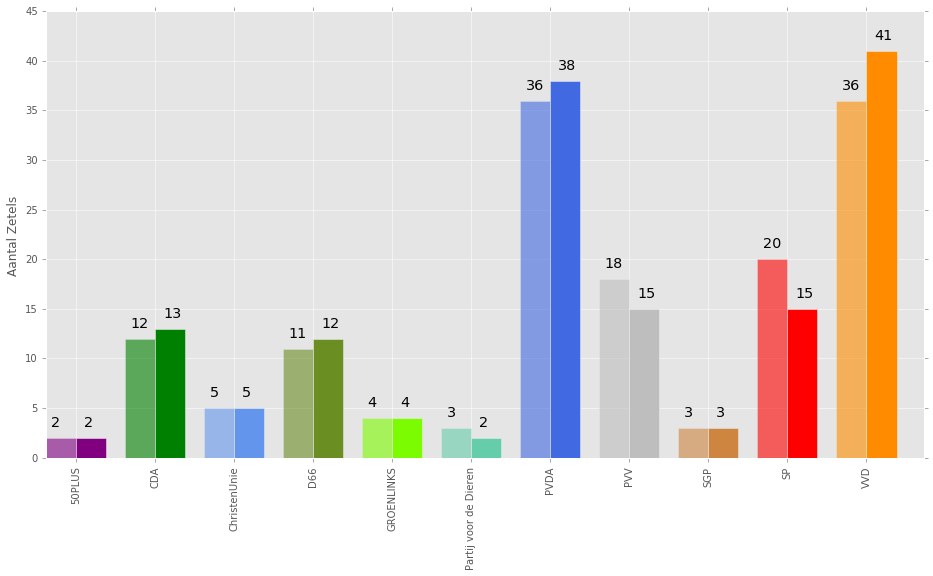
\includegraphics[width=\linewidth]{peiling_zetels_landelijk.png}

			\caption{De zetelverdelingen (licht gekleurd) volgens de peiling van 11 september 2012 \citep{IPSOS} en volgens de offici\"{e}le einduitslag (donker gekleurd) van 12 september 2012 \citep{Kiesraad_databank}.}

\label{fig:pzL}
\end{figure}











\subsection{Datasets betreffende de Bevolkingsgroep Vrouwen.}
De datasets betreffende de bevolkingsgroep vrouwen zijn:\\




\newcolumntype{L}{@{}>{\bfseries}p{13em}<{}}% Item label
\newcolumntype{I}{X@{}}% Item contents
\noindent\begin{tabularx}{\textwidth}{LI}
Geslacht: & Geslacht van de kandidaten op de kandidatenlijsten van de partijen \cite{Kiesraad_kandidatenlijsten}. In de grafiek in Figuur \ref{fig:mvKandidaten} is het aantal mannelijke en vrouwelijke kandidaten op de kandidatenlijsten van de partijen te zien. Het gaat hierbij om enkel om partijen die volgens de peiling zetels zouden gaan ontvangen.\\
\\
Man-vrouw stemmenverdeling: & Man-vrouw verdeling in percentage van het totaal aantal uitgebrachte stemmen op een partij op basis van de einduitslag \citep{IPSOS}. In Tabel \ref{table:tab2V} (zie Sectie \ref{sssec:vrouwen}) zijn de mannelijke een vrouwelijke stempercentages te zien. \\
\\  
\end{tabularx}

\newcolumntype{L}{@{}>{\bfseries}p{13em}<{}}% Item label
\newcolumntype{I}{X@{}}% Item contents
\noindent\begin{tabularx}{\textwidth}{LI}
Ontbrekende data:  & Vanwege het ontbreken van data betreffende een peiling onder vrouwelijke kiezers nemen we aan dat de landelijke peiling toereikend is voor de peiling onder vrouwelijke kiezers. Zodoende gebruiken we de dataset met daarin de landelijke peiling als dataset voor de peiling onder vrouwelijke kiezers. \\
  \\
\end{tabularx}
\begin{figure}[H]
\centering
	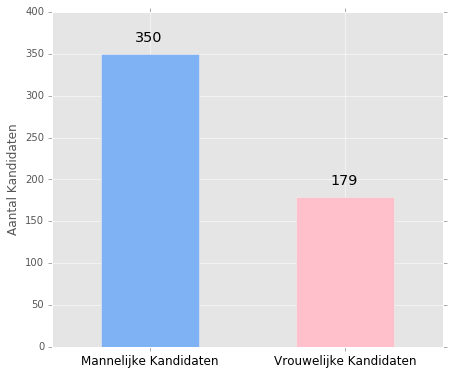
\includegraphics[width=0.42\linewidth]{mv_kandidaten.png}

			\caption{Het aantal mannelijke en vrouwelijk kandidaten op de kandidatenlijsten van de partijen die volgens de peiling zetels zouden gaan ontvangen.}

\label{fig:mvKandidaten}
\end{figure}



\subsection{Datasets betreffende de Bevolkingsgroep Allochtonen.}
De datasets betreffende de bevolkingsgroep allochtonen zijn:\\



\newcolumntype{L}{@{}>{\bfseries}p{13em}<{}}% Item label
\newcolumntype{I}{X@{}}% Item contents
\noindent\begin{tabularx}{\textwidth}{LI}
Peiling onder allochtonen: & Peiling onder westerse en niet-westerse allochtonen \citep{Opiniehuis}. In Tabel \ref{table:tab1A} (zie Sectie \ref{sssec:allochtonen}) is de verdeling volgens de peiling in percentages te zien.\\
\\
Bevolkingsaantallen: & Bevolkingsaantallen van westerse en niet-westerse allochtonen in Nederland \citep{CBS_allochtonen}. Op 1 september 2012 waren er 2.629.699 allochtonen boven de 18 jaar wonenden in Nederland. We gaan er voor deze bevolkingsgroep vanuit dat al deze personen stemgerechtigd waren tijdens de Tweede Kamerverkiezingen van 2012. \\
\\  
Stemgedrag:  & Stemgedrag van westerse en niet-westerse allochtonen \citep{CBS_stemgedrag}. Hierbij staat het aandeel allochtone stemmen op een partij tot verhouding met het totaal aantal uitgebrachte allochtone stemmen bij de Tweede Kamerverkiezingen. Dit noemen we het allochtone stempercentage. In de grafiek in Figuur \ref{table:tab2A} (zie Sectie \ref{sssec:allochtonen}) is op basis van de einduitslag de stemverdeling in percentages te zien.\\
 \\
\end{tabularx}

\newcolumntype{L}{@{}>{\bfseries}p{13em}<{}}% Item label
\newcolumntype{I}{X@{}}% Item contents
\noindent\begin{tabularx}{\textwidth}{LI}
Allochtone kandidaten: & De allochtone kandidaten op de kandidatenlijsten van de partijen. Hierbij moet genoteerd worden dat deze dataset deels zelf in elkaar is gezet. Onderzoeken van \citet{marinissen2013stemmen} en het Sio \citeyear{SIO} leverde al 33 allochtone kandidaten op. Echter waren deze kandidaten enkel van Marokkaanse, Turkse of Surinaamse afkomst. Voor de andere kandidaten is er ten behoeve van dit onderzoek gekeken of zij allochtoon zijn of niet. Hierbij zijn online bronnen geraadpleegd. In het geval dat twee of meerdere online bronnen aangaven dat een kandidaat als allochtoon geïdentificeerd kon worden, is de kandidaat toegevoegd aan de dataset. Het is daarom belangrijk te benadrukken dat er niet met 100\% zekerheid gesteld kan worden of een kandidaat allochtoon is of niet. Ter illustratie van het tot stand komen van de dataset nemen we Vera Bergkamp van D66 en Jenny Zerfowski van de PVV als voorbeelden.

\indent Vera Bergkamp heeft een, op het eerst gezicht, naam die niet snel aan een buitenlandse afkomst doet denken. Echter heeft Vera Bergkamp volgens \citet{allochtonie} en volgens \citet{zaman} een Marokaanse vader. Volgens de definitie van het CBS (zie VERWIJZING NAAR INTRODUCTIE) is Vera Bergkamp een allochtoon. Het volgende voorbeeld is Jenny Zerfowski van de PVV. Jenny Zerfowski heeft, in tegenstelling tot Vera Bergkamp, wel een buitenlands klinkende achternaam. Om haar enkel op basis van haar achternaam te identificeren als allochtoon zou niet toereikend zijn. Daarnaast is het de vraag of dit wel ethisch verantwoord is. Hoe dan ook is er ten behoeve van dit onderzoek gepoogd uit te zoeken of Jenny Zerfowski een allochtoon is. Volgens een artikel in de Volkskrant\citeyearpar{volkskrantjenny} en een interview met haar op \citet{binnenlandsbestuur} is Jenny Zerfowski in Duitsland geboren. Op deze wijze zijn er vijftig kandidaten als allochtoon geïdentificeerd. In de grafiek in Figuur \ref{fig:aaKandidaten} is het aantal autochtone en allochtone kandidaten te zien.\\
  \\
\end{tabularx}







\iffalse
\begin{figure}[H]
\centering
	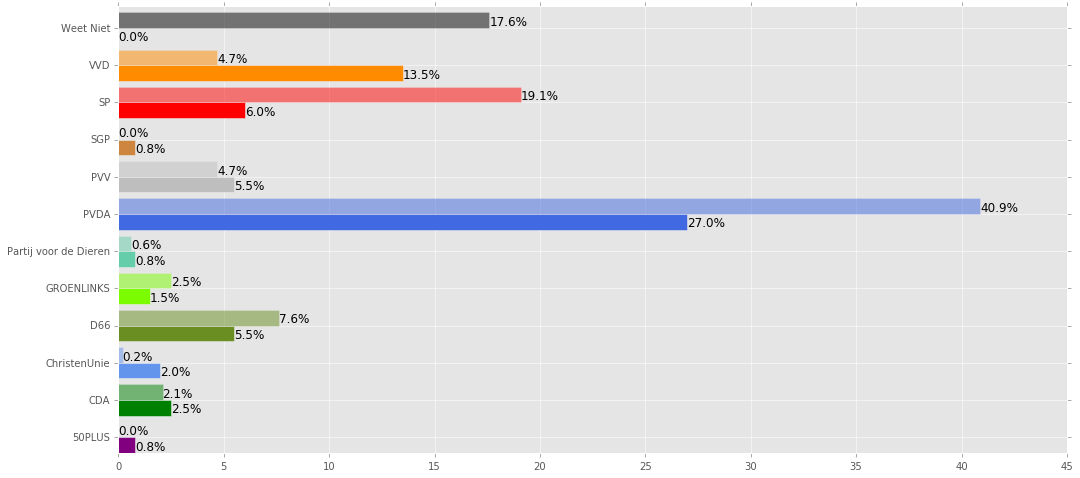
\includegraphics[width=\linewidth]{peiling_uitslag_percentages_allochtonen.png}

			\caption{De verdeling in procenten van allochtone stemmen op de partij volgens de peiling (licht gekleurd) en volgens de einduitslag (donker gekleurd).}

\label{fig:peil_uit_aa}
\end{figure}
\fi


\begin{figure}[H]
\centering
	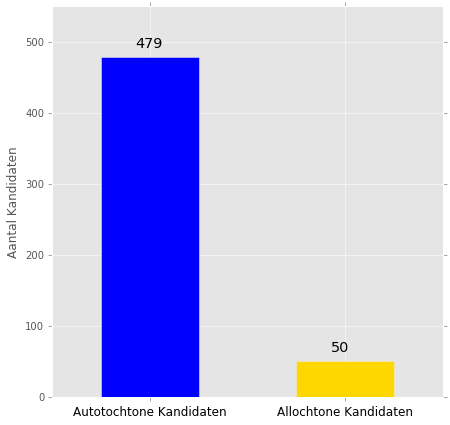
\includegraphics[width=0.42\linewidth]{aa_kandidaten.png}

			\caption{Het aantal autochtone en allochtone kandidaten op de kandidatenlijsten van de partijen die volgens de peiling zetels zouden gaan ontvangen.}

\label{fig:aaKandidaten}
\end{figure}


\subsection{Datasets betreffende de Bevolkingsgroep Ouderen.}
De datasets betreffende de bevolkingsgroep ouderen zijn:\\

\newcolumntype{L}{@{}>{\bfseries}p{13em}<{}}% Item label
\newcolumntype{I}{X@{}}% Item contents
\noindent\begin{tabularx}{\textwidth}{LI}
Bevolkingsaantallen: &Bevolkingsaantallen van ouderen \citep{CBS_allochtonen}. De bevolkingsaantallen van alle personen van vijftig jaar een ouder wonenden in Nederland op 1 september 2012. We nemen hierbij aan dat al deze personen stemgerechtigd zijn.   \\
\\  
Stemgedrag:  & Stemgedrag van ouderen \citep{CBS_stemgedrag}. Hierbij staat het aandeel oudere stemmen op een partij tot verhouding met het totaal aantal uitgebrachte oudere stemmen bij de Tweede Kamerverkiezingen. Dit noemen we het oudere stempercentage. \\
\\
Oudere kandidaten: & De oudere kandidaten op de kandidatenlijsten van de partijen \citep{allekandidaten}. Zie de grafiek in Figuur \ref{fig:jaKandidaten} voor het aantal kandidaten met een leeftijd van 50 jaar of jonger en het aantal oudere kandidaten op de kandidatenlijsten van de partijen die volgens de peiling zetels zouden gaan ontvangen. \\
  \\
Ontbrekende data: &  Vanwege het ontbreken van een peiling onder oudere kiezers nemen we aan de landelijk peiling toereikend is voor de peiling onder oudere kiezers. Zodoende gebruiken we de dataset met daarin de landelijk peiling als dataset voor de peiling onder oudere kiezers.\\
\\
 \end{tabularx}


\begin{figure}[H]
\centering
	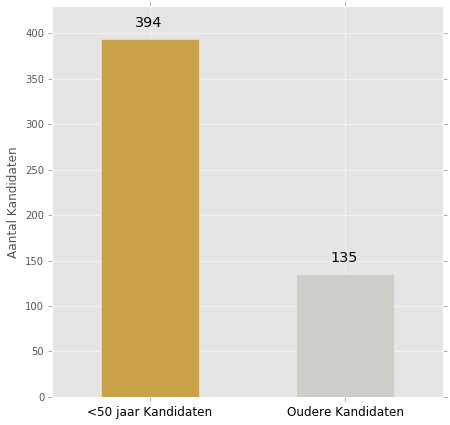
\includegraphics[width=0.42\linewidth]{ja_kandidaten.png}

			\caption{Het aantal kandidaten met een leeftijd van 50 jaar of jonger en het aantal oudere kandidaten op de kandidatenlijsten van de partijen die volgens de peiling zetels zouden gaan ontvangen.}

\label{fig:jaKandidaten}
\end{figure}


\newpage
\subsection{Datasets betreffende de Bevolkingsgroep Provincialen.}
De datasets betreffende de provincialen ouderen zijn:\\

\newcolumntype{L}{@{}>{\bfseries}p{13em}<{}}% Item label
\newcolumntype{I}{X@{}}% Item contents
\noindent\begin{tabularx}{\textwidth}{LI}
De Randstad-gemeenten: &  Er is in de literatuur geen eenduidige stelling over welke gemeenten precies tot de Randstad behoren. Daarmee is de exacte grens moeilijk vast te stellen \citep{nijmeijer2000randstad}. Daarom is de dataset met daarin de Randstad-gemeenten verkregen van Wikipedia \citeyearpar{randstad}. Hierbij is een kleine steekproef uitgevoerd om zodoende uit te vinden of een gemeente in de dataset daadwerkelijk tot de Randstad gerekend kan worden. Ter illustratie nemen we de gemeente Haarlem en vervolgens de gemeente Woerden als voorbeelden. 

\hspace*{1em} Voor de gemeente Haarlem is in twee verschillende online bronnen gevonden waarin er wordt gesteld dat de gemeente Haarlem in de Randstad ligt. Deze bronnen zijn de Trouw \citeyear{trouwhaarlem} en HP/De Tijd \citeyear{HPhaarlem}. Ook voor de gemeente Woerden is er in twee verschillende online bronnen gevonden dat er gesteld wordt dat de gemeente Woerden in de Randstad ligt. Deze bronnen zijn de gemeente Woerden \citeyear{gemeentewoerden} en Villa-Berlage \citeyear{villaberlage}. Op dezelfde wijze als voor deze twee gemeenten is gedaan, is dit ook voor de een aantal andere gemeenten in de dataset gedaan. Alle gemeenten die zijn meegenomen in de steekproef bevinden zich, volgens verschillende online bronnen, in de Randstad. Zodoende bleek uit de steekproef dat de dataset met daarin gemeenten in de Randstad een grote mate van betrouwbaarheid geniet. Via de Kiesraad \citeyearpar{Kiesraad_databank} is achterhaald hoeveel stemgerechtigden er in de Randstad-gemeenten woonden ten tijde van de Tweede Kamerverkiezingen van 2012.  \\
\\  
Aantal stemgerechtigden:  & Het aantal stemgerechtigde provincialen is tot stand gekomen door alle stemgerechtigden uit de Randstad-gemeenten \citep{randstad} af te trekken van het totaal aantal stemgerechtigden in Nederland ten tijde van de Tweede Kamerverkiezingen van 2012 \citep{Kiesraad_uitslag}.   \\
\\
Provinciale kandidaten: &  Voor het vaststellen of een kandidaat als provinciale kandidaat geïdentificeerd kan worden, is weer de dataset met daarin alle Randstad-gemeenten gebruikt \citep{randstad}. Door Randstad-gemeenten dataset te combineren met de kandidatenlijsten (hierin staan ook de woonplaatsen van de kandidaten) is er vastgesteld welke kandidaten wel en welke kandidaten er niet uit de Randstad-gemeenten afkomstig zijn.  Zie de grafiek in Figuur \ref{fig:rpKandidaten} voor het aantal Randstedelijke en provinciale kandidaten op de kandidatenlijsten van de partijen die volgens de peiling zetels zouden gaan ontvangen.\\
\\
 \end{tabularx}


\newcolumntype{L}{@{}>{\bfseries}p{13em}<{}}% Item label
\newcolumntype{I}{X@{}}% Item contents
\noindent\begin{tabularx}{\textwidth}{LI}
Ontbrekende data: &   Vanwege het ontbreken van data betreffende een peiling onder provinciale kiezers nemen we aan dat de landelijke peiling toereikend is voor de peiling onder provinciale kiezers. Zodoende gebruiken we de dataset met daarin de landelijke peiling als dataset voor de peiling onder provinciale kiezers.

\hspace*{1em} Naast het ontbreken van een peiling onder provincialen, ontbreekt ook de data betreffende het aandeel provinciale stemmen op een partij in verhouding tot het totaal aantal uitgebrachte provinciale stemmen bij de Tweede Kamerverkiezingen. Zodoende gebruiken we het landelijk stempercentage als stempercentage voor de provinciale stemmen.\\
\\
 \end{tabularx}



\begin{figure}[H]
\centering
	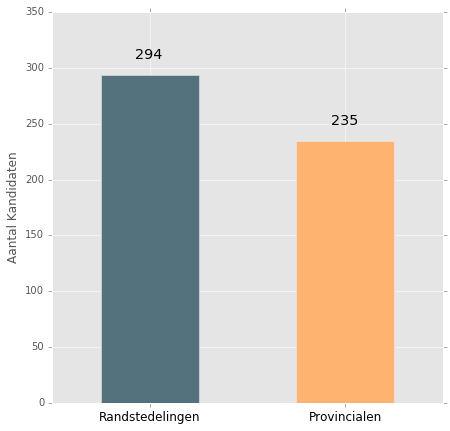
\includegraphics[width=0.42\linewidth]{rp_kandidaten.png}

			\caption{Het aantal Randstedelijke en provinciale kandidaten op de kandidatenlijsten van de partijen die volgens de peiling zetels zouden gaan ontvangen.}

\label{fig:rpKandidaten}
\end{figure}

















\iffalse

Data verzameling en beschrijving van de data jajaja

Hoe is de data verzameld, en hoe heb jij die data verkregen?


Wat staat er in de data? Niet alleen maar een technisch verhaal, maar ook inhoudelijk. DE lezer moet een goed idee krijgen over de technische inhoud en wat het betekent.

\newpage


\pagebreak
\subsection{Wat plotjes en tabelletjes}

Zie het IPython Notebook \url{PandasAndLatex.ipynb} voor de code om vanuit pandas een poltje op te slaan en een dataframe als tabel op te slaan. Het werkt ideaal! 

%De interrupties van Wilders staan beschreven in Figure~\ref{fig:wilders} en Tabel~~\ref{tab:Wilders}.


%\begin{figure}
%\begin{center}
%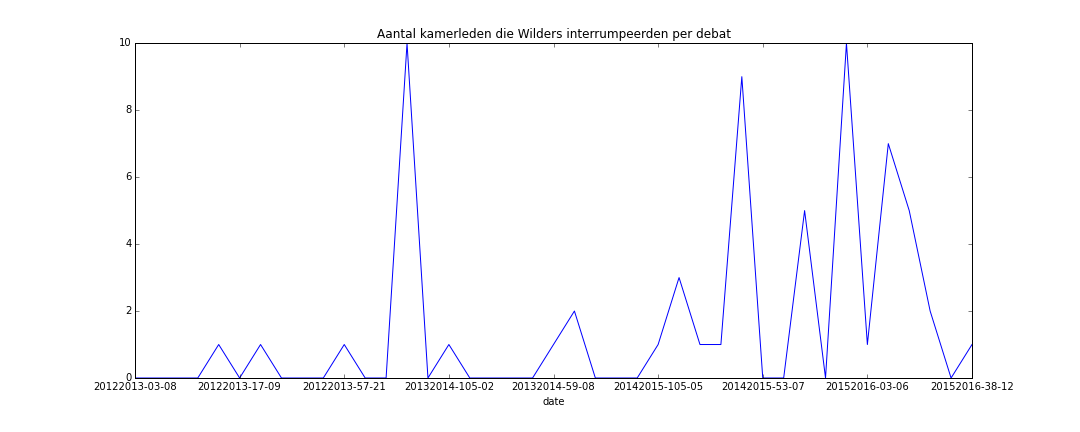
\includegraphics[width=\linewidth]{WildersPlot.png}
%\caption{\label{fig:wilders} Aantal interrupties van Wilders in de Tweede Kamer %door de tijd (periode 2012-2016).}
%\end{center}
%\end{figure}



\pagebreak


%\begin{table}[h]
%\begin{footnotesize}
%\begin{tabular}{lrl}
\toprule
{} &  indegree &                               interruptie\_volgorde \\
date            &           &                                                    \\
\midrule
20122013-03-08  &         0 &                                                    \\
20122013-07-16  &         0 &                                                    \\
20122013-100-03 &         0 &                                                    \\
20122013-100-06 &         0 &                                                    \\
20122013-17-06  &         1 &                         Pechtold-Pechtold-Pechtold \\
20122013-17-09  &         0 &                                                    \\
20122013-21-04  &         1 &                         Pechtold-Pechtold-Pechtold \\
20122013-22-08  &         0 &                                                    \\
20122013-32-06  &         0 &                                                    \\
20122013-48-23  &         0 &                                                    \\
20122013-57-21  &         1 &  Pechtold-Pechtold-Pechtold-Pechtold-Pechtold-P... \\
20122013-76-03  &         0 &                                                    \\
20122013-76-06  &         0 &                                                    \\
20132014-05-02  &        10 &  Roemer-Roemer-Van Haersma Buma-Van Haersma Bum... \\
20132014-06-04  &         0 &                                                    \\
20132014-105-02 &         1 &  Pechtold-Pechtold-Pechtold-Pechtold-Pechtold-P... \\
20132014-105-06 &         0 &                                                    \\
20132014-14-03  &         0 &                                                    \\
20132014-14-06  &         0 &                                                    \\
20132014-52-18  &         0 &                                                    \\
20132014-59-08  &         1 &                               Klaver-Klaver-Klaver \\
20142015-02-08  &         2 &  Pechtold-Pechtold-Pechtold-Pechtold-Pechtold-P... \\
20142015-03-06  &         0 &                                                    \\
20142015-09-09  &         0 &                                                    \\
20142015-100-05 &         0 &                                                    \\
20142015-105-05 &         1 &                                  Pechtold-Pechtold \\
20142015-111-04 &         3 &  Pechtold-Pechtold-Pechtold-Pechtold-Pechtold-P... \\
20142015-111-07 &         1 &                                  Pechtold-Pechtold \\
20142015-39-71  &         1 &                                  Pechtold-Pechtold \\
20142015-41-07  &         9 &  Samsom-Samsom-Pechtold-Pechtold-Pechtold-Kuzu-... \\
20142015-53-07  &         0 &                                                    \\
20142015-61-23  &         0 &                                                    \\
20142015-79-07  &         5 &  Klaver-Klaver-Klaver-Gesthuizen-Gesthuizen-Ges... \\
20142015-95-06  &         0 &                                                    \\
20152016-02-07  &        10 &  Pechtold-Pechtold-Pechtold-Pechtold-Slob-Slob-... \\
20152016-03-06  &         1 &       Pechtold-Pechtold-Pechtold-Pechtold-Pechtold \\
20152016-14-02  &         7 &  Klaver-Klaver-Roemer-Roemer-Roemer-Roemer-Sams... \\
20152016-14-05  &         5 &  Van Haersma Buma-Van Haersma Buma-Van Haersma ... \\
20152016-27-03  &         2 &  Segers-Segers-Segers-Segers-Kuzu-Kuzu-Kuzu-Kuz... \\
20152016-38-10  &         0 &                                                    \\
20152016-38-12  &         1 &                                        Klein-Klein \\
\bottomrule
\end{tabular}

%\end{footnotesize}
%\caption{\label{tab:Wilders} Door wie werd Wilders onderbroken en hoe vaak per debat.}
%\end{table}

%\begin{table}[h]
%	\begin{footnotesize}
%		\begin{tabular}{lrr}
\toprule
{} &  Aantal Stemmen Partij &  Aantal Stemmen Van Vrouwen \\
Partij                &                        &                             \\
\midrule
50PLUS                &                 123514 &                       61757 \\
CDA                   &                 741084 &                      370542 \\
ChristenUnie          &                 308785 &                      154392 \\
D66                   &                 679327 &                      339663 \\
GROENLINKS            &                 247028 &                      123514 \\
Partij v d Dieren &                 185271 &                       92635 \\
PVDA                  &                2223254 &                     1111627 \\
PVV                   &                1111627 &                      555813 \\
SGP                   &                 185271 &                       92635 \\
SP                    &                1235141 &                      617570 \\
VVD                   &                2223254 &                     1111627 \\
\bottomrule
\end{tabular}

%	\end{footnotesize}
%		\caption{\label{tab:Figuur1} Door wie werd Wilders onderbroken en hoe vaak per debat.}
%\end{table}

\pagebreak
\subsection{Methods}
Hoe je je vraag gaat beantwoorden.


Dit is de langste sectie van je scriptie. 

Als iets erg technisch wordt kan je een deel naar de Appendix verplaatsen. 

Probeer er een lopend verhaal van te maken.

Het is heel handig dit ook weer op te delen nav je deelvragen:

\subsubsection{RQ1}

\subsubsection{RQ2}
\fi

\newpage
\section{Theoretisch Maximum}
\label{sec:eva}

\titlespacing*{\subsubsection}{0pt}{30pt}{10pt}


\subsection*{Deelvraag 1: Wat is het theoretisch maximum aantal kandidaten dat per specifieke bevolkingsgroep in de Tweede Kamer gekozen had kunnen worden bij de verkiezingen van 2012?}

Om het theoretisch maximum te gaan berekenen zullen we als eerst kijken naar de verschillende specifieke bevolkingsgroepen zoals we deze hebben bepaald in de Hoofdstuk \ref{sec:intro}. Deze bevolkingsgroepen zijn: vrouwen, allochtonen, ouderen(met de leeftijd van vijftig jaar en ouder) en provincialen (Nederlanders van buiten de Randstad). 


\paragraph*{Resultaten strategie\"{e}n per bevolkingsgroep.} 
In Tabel \ref{table:S_overzicht} en Figuur \ref{fig:S_overzicht} hieronder zijn per bevolkingsgroep de resultaten van de verschillende strategie\"{e}n te zien. We zien dat strategie 1 voor alle vier de bevolkingsgroepen een hoog rendement zou hebben opgeleverd. Echter zou strategie 4 voor de provincialen het hoogste rendement hebben opgeleverd (zie \hyperref[S4P]{strategie 4} van \hyperref[provincialen]{Bevolkingsgroep: Provincialen} in Bijlage \ref{b1}). Strategie 2 zou bij alle vier de bevolkingsgroepen ook een hoog rendement hebben opgeleverd. Bij de allochtonen zou het zelfs geen verschil hebben uitgemaakt of strategie 1 of strategie 2 zou zijn uitgevoerd. Het rendement is hetzelfde. Strategie 3.1, strategie 3.2 en strategie 4 zijn op bij de bevolkingsgroep allochtonen niet toegepast vanwege een te klein aantal allochtone kandidaten om uitvoering van deze strategie\"{e}n mogelijk te maken.  

De verschillende strategie\"{e}n worden in dit hoofdstuk in Sectie \ref{vrouwen} toegepast op de bevolkingsgroep vrouwen. Bij deze bevolkingsgroep worden de strategie\"{e}n tot in detail uitgelegd en ondersteund met enkele voorbeelden. Ten behoeve van de leesbaarheid zijn de andere drie bevolkingsgroepen naar Bijlage \ref{b1} verplaatst. Tevens wordt in de bijlage van deze bevolkingsgroepen enkel het resultaat en de analyse getoond. Voor een getailleerde uitleg van uitwerking van de strategie\"{e}n, ga naar Sectie \ref{vrouwen} of ga anders door naar Hoofdstuk \ref{h5}

\begin{table}[h]
\captionsetup{skip=-2pt}
\begin{center}
\begin{footnotesize}
\begin{tabular}{lrrrrr}
\toprule
{} &  Strategie 1 &  Strategie 2 &  Strategie 3.1 &  Strategie 3.2 &  Strategie 4 \\
\midrule
Vrouwen      &         121 &          116 &             91 &            101 &          121 \\
Allochtonen  &           34 &           34 &            n.v.t. &           n.v.t. &          n.v.t. \\
Ouderen      &           89 &           84 &             77 &             69 &           89 \\
Provincialen &          138 &          131 &            103 &            120 &          142 \\
\bottomrule
			
			
\end{tabular}
\end{footnotesize}
\end{center}
\caption{Overzicht van de resultaten per bevolkingsgroep in aantal zetels per strategie.}
\label{table:S_overzicht} 
\end{table}


\begin{figure}[H]
\captionsetup{skip=0pt}

	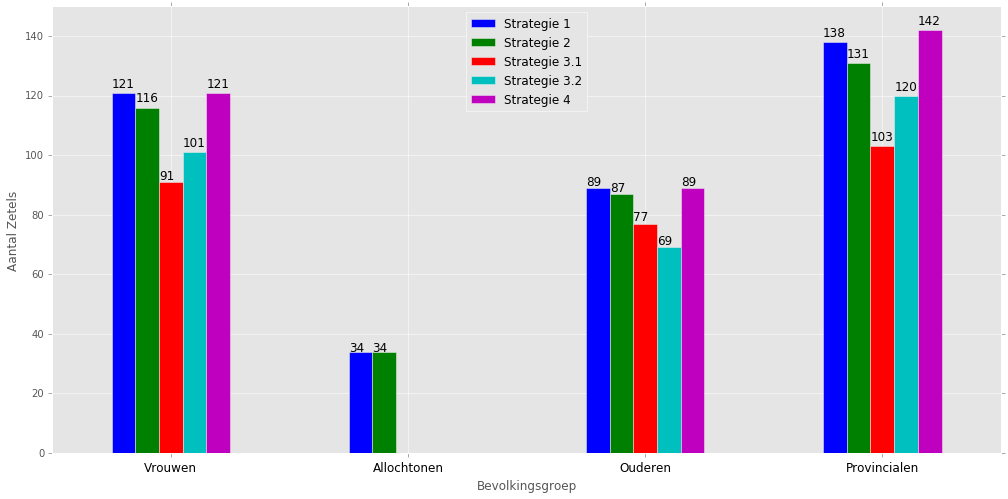
\includegraphics[width=0.95\linewidth]{overzicht_resultaten_strategien_plot1.png}

			\caption{Grafiek met overzicht van de resultaten in aantal zetels per strategie en per bevolkingsgroep.}

\label{fig:S_overzicht}
\end{figure}


\subsection{Bevolkingsgroep: Vrouwen.}
\label{vrouwen}
Betreffende de bevolkingsgroep vrouwen in Nederland worden hieronder verschillende strategie\"{e}n uiteengezet. Zodoende pogen we te achterhalen hoe in theorie de meeste vrouwelijke kandidaten in de Tweede Kamer gekozen hadden kunnen worden wanneer alle stemgerechtigde vrouwelijke kiezers in Nederland zich hadden gecommitteerd aan een strategie (zie Bijlage \ref{b1} voor de drie andere bevolkingsgroepen). In Sectie \ref{percV} wordt er onderzocht wat er zou zijn gebeurd wanneer een deel van de bevolkingsgroep zich had gecommitteerd aan een strategie. 

\paragraph{Het berekenen van het aantal te verwachten vrouwelijke stemmen.}
Voor het opzetten van de strategie\"{e}n en het, voor elke strategie, kunnen toewijzen van de stemmen van vrouwelijke kiezers aan de vrouwelijke kandidaten van de partijen moeten we eerst weten hoeveel stemmen de partijen volgens de peiling zou gaan ontvangen. Dit doen we door de verwachte opkomst te delen door het aandeel zetels (in een percentage) dat een partij volgens de peiling zou gaan ontvangen. Ter illustratie het volgende voorbeeld: In de peiling van 11 september 2012 \citep{IPSOS} werd er een opkomst van 73\% van alle stemgerechtigden verwacht. Er waren in 2012 een totaal aantal van 12.689.810 stemgerechtigden \citep{Kiesraad_uitslag}. Dat betekent dat 73\% van alle stemgerechtigden uitkomt op ($0,73*12.689.810$ = ) 9.263.561 te verwachten stemmen. Het aantal stemmen die een partij zou gaan ontvangen is dus het aandeel van het aantal zetels in de Tweede Kamer dat een partij zou gaan ontvangen volgens de peiling. Ter illustratie het volgende voorbeeld: de PVDA  zou, volgens de peiling,  36 zetels ontvangen. Dat komt neer op een percentage van ($36\div150$ zetels = ) 24\% van alle zetels. Het aantal stemmen dat de PVDA daarmee zou gaan ontvangen is dan het aantal van ($0,24*9.263.561$ = ) 2.223.254 stemmen. We nemen aan dat de man-vrouw stemmenverdeling bij elke partij gelijk is. Oftewel de helft van de stemmen die een partij ontvangt komt van mannen en de andere helft van de stemmen komt van vrouwen. Daarmee zal de PVDA het totale aantal van ($0,50*2.223.254$ = ) 1.111.627 stemmen van vrouwelijke kiezers gaan ontvangen. In Tabel \ref{table:tab1V} hieronder is o.a. te zien hoeveel stemmen de partijen, volgens de peiling, zouden gaan ontvangen van vrouwelijke kiezers. Naast het berekenen van het aantal te verwachten stemmen per partij kunnen we ook de te verwachten voorkeursdrempel berekenen. Zoals eerder al is toegelicht, is de voorkeursdrempel 25\% van de kiesdeler. De kiesdeler is het aantal stemmen dat genoeg is voor één zetels. De te verwachten kiesdeler is het aantal van ($9.263.561\div150$ = ) 61.757 stemmen. De te verwachten voorkeursdrempel wordt daarom vastgesteld op het aantal van ($0,25*61.757$ = ) 15.439 stemmen.






\begin{table}[h]
\centering
	\begin{footnotesize}
		\begin{tabular}{lrr}
\toprule
{} &  Aantal Stemmen Partij &  Aantal Stemmen Van Vrouwen \\
Partij                &                        &                             \\
\midrule
50PLUS                &                 123514 &                       61757 \\
CDA                   &                 741084 &                      370542 \\
ChristenUnie          &                 308785 &                      154392 \\
D66                   &                 679327 &                      339663 \\
GROENLINKS            &                 247028 &                      123514 \\
Partij v d Dieren &                 185271 &                       92635 \\
PVDA                  &                2223254 &                     1111627 \\
PVV                   &                1111627 &                      555813 \\
SGP                   &                 185271 &                       92635 \\
SP                    &                1235141 &                      617570 \\
VVD                   &                2223254 &                     1111627 \\
\bottomrule
\end{tabular}

	\end{footnotesize}
			\caption{Totaal aantal stemmen dat een partij zou gaan ontvangen en het totaal aantal te verwachte vrouwelijke stemmen volgens de peiling \citep{IPSOS}.}
\label{table:tab1V} 
\end{table}

\newpage
\paragraph{Het berekenen van het werkelijke aantal vrouwelijke stemmen.}
Voor het bepalen van het rendement van een strategie en het berekenen van het aantal stemmen dat een partij van vrouwelijke kiezers had ontvangen, kijken we eerst naar het totaal aantal stemmen die de partijen volgens de einduitslag hebben ontvangen \citep{Kiesraad_uitslag}. Ook kijken we naar de vrouw-man verdeling van het aantal stemmen op de partijen \citep{IPSOS_man_vrouw}. Ter illustratie het volgende voorbeeld: de PVDA had bij de einduitslag een totaal van 2.340.750 stemmen ontvangen. Hiervan kwamen 52\% van de stemmen van vrouwelijke kiezers. Dit betekent dat de PVDA volgens de einduitslag het aantal van ($0,52*2.340.750$ = ) 1.217.190 stemmen van vrouwelijk kiezers had ontvangen. De vrouwelijke stemmen die een partij had ontvangen worden vervolgens willekeurig verdeeld over een \textit{N} aantal vrouwelijke kandidaten. Omdat de \textit{N} aantal vrouwen per strategie en vervolgens per partij telkens anders is wordt er later per strategie aan de hand van voorbeelden uitgelegd hoe de vrouwelijke stemmen die een partij had ontvangen zouden zijn toegewezen aan de \textit{N} vrouwelijke kandidaten van de partij. Hieronder is tabel \ref{table:tab2V} per partij te zien hoeveel stemmen de partij in totaal had ontvangen, hoeveel procent van de stemmen van vrouwelijke kiezers kwamen, hoeveel procent de stemmen van mannelijk kiezers kwamen en het aantal stemmen dat de partij van vrouwelijke kiezers had ontvangen. 


\begin{table}[h]
\centering
	\begin{footnotesize}
		\begin{tabular}{lrrrr} 
\toprule 
{} &  Aantal Stem-  &  Vrouwelijke Stem- &  Mannelijke Stem-  &  Aantal Stemmen  \\
Partij                &        men Partij              &                                men Percentage &            men Percentage                  &    Van Vrouwen                         \\
\midrule
50PLUS                &                 177631 &                              51 &                             49 &                       90591 \\
CDA                   &                 801620 &                              40 &                             60 &                      320648 \\
ChristenUnie          &                 294586 &                              63 &                             37 &                      185589 \\
D66                   &                 757091 &                              42 &                             58 &                      317978 \\
GROENLINKS            &                 219896 &                              48 &                             52 &                      105550 \\
Partij v d Dieren &                 182162 &                              51 &                             49 &                       92902 \\
PVDA                  &                2340750 &                              52 &                             48 &                     1217190 \\
PVV                   &                 950263 &                              44 &                             56 &                      418115 \\
SGP                   &                 196780 &                              51 &                             49 &                      100357 \\
SP                    &                 909853 &                              57 &                             43 &                      518616 \\
VVD                   &                2504948 &                              43 &                             57 &                     1077127 \\
\bottomrule
\end{tabular}

	\end{footnotesize}

			\caption{Totaal aantal stemmen dat een partij heeft ontvangen \citep{Kiesraad_databank} de vrouw-man verdeling van de stemmen in percentages \citep{IPSOS_man_vrouw} en het totaal aantal vrouwelijke stemmen wat de partijen daarmee hebben ontvangen.}
\label{table:tab2V} 
\end{table}




\paragraph{Het uiteindelijk opstellen van de Tweede Kamer na uitvoering van een strategie.} \label{opstellen}
Nadat bij elke strategie de stemmen van vrouwelijke kiezers per partij zijn toegewezen aan de vrouwelijke kandidaten van de partij moet de nieuwe Tweede Kamer worden opgesteld. Het opstellen van de Tweede Kamer voltrekt zich conform de regels
zoals door de Kiesraad \citeyearpar{Kiesraad_voorkeursdrempel2} wordt toegepast
en gaat als volgt: 

\begin{itemize}
	\item
\textbf{Stap 1:} Als eerst wordt er gekeken hoeveel zetels een partij had ontvangen bij de uitslag van de Tweede Kamerverkiezingen van 2012. 
	\item
\textbf{Stap 2:} Vervolgens wordt, na toewijzing van de stemmen van vrouwelijke kiezers op vrouwelijke kandidaten, geteld hoeveel kandidaten (vrouwelijke én mannelijke kandidaten) er boven de kiesdrempel uitgekomen zouden zijn. Daarbij moet genoteerd worden dat na uitvoering van de strategie de mannelijke kandidaten een even groot aantal stemmen hebben ontvangen als in werkelijkheid het geval was. De reden hiervoor is dat het theoretisch mogelijk is dat de mannelijke kandidaten enkel stemmen hadden ontvangen van mannelijke kiezers. Ook al is dit onwaarschijnlijk, we kunnen dit niet weten en zullen dan ook geen stemmen van de mannelijke kandidaten aftrekken. Derhalve is het aantal stemmen dat een mannelijke kandidaat zou hebben ontvangen na uitvoering van een strategie hetzelfde als bij de daadwerkelijke verkiezingsuitslag van 2012.
	\item
\textbf{Stap 3:} Nadat we, na uitvoering van een strategie, hebben geteld hoeveel kandidaten genoeg stemmen zouden hebben ontvangen om aan de voorkeursdrempel te voldoen kijken we per partij of de partij een groter aantal zetels heeft ontvangen dan het aantal kandidaten van de partij die boven de voorkeursdrempel gekomen zouden zijn. 
	\item
\textbf{Stap 4:} Als de partij meer zetels had ontvangen dan er voor de partij kandidaten boven de voorkeursdrempel gekomen zouden zijn, worden de resterende zetels vergeven aan de hoogst genoteerde kandidaten op de kandidatenlijst van de partij (mits deze kandidaten dus niet genoeg stemmen zouden hebben ontvangen om boven de voorkeursdrempel uit te komen).
\end{itemize}


\subsubsection*{Beschrijving Strategie\"{e}n} \label{besS}
In deze sectie zullen vijf strategie\"{e}n worden beschreven waarbij de aannames voor elke strategie hetzelfde zijn. Deze aannames zijn:

\begin{itemize}
	\item 
Alle stemgerechtigde vrouwen waarvan de peiling aangaf dat zij zouden gaan stemmen hebben meegedaan aan de strategie.
	\item
Vrouwelijke kiezers hebben daarbij volstrekt willekeurig gestemd op de top \textit{N} vrouwelijke kandidaten van de partij waar zij toch al op wilden stemmen.	
	\item
Alle stemgerechtigde mannen waarvan de peiling aangaf dat zij zouden gaan stemmen hebben niet meegedaan aan de strategie en hebben ook geen eigen (tegen)strategie bepaald. Mannelijke kiezers hebben derhalve hetzelfde gestemd zoals zij volgens de einduitslag hebben gedaan. 
\end{itemize}


\noindent Voordat we de strategie\"{e}n op de bevolkingsgroep vrouwen gaan toepassen worden hieronder de vijf strategie\"{e}n beknopt beschreven:\\


\newcolumntype{L}{@{}>{\bfseries}p{16em}<{}}% Item label
\newcolumntype{I}{X@{}}% Item contents
\noindent\begin{tabularx}{\textwidth}{LI}
  Strategie 1. Top \textit{N} volgens de peiling: & Vrouwelijk kiezers stemmen volstrekt willekeurig op een top \textit{N}  vrouwelijke kandidaat waarbij \textit{N} wordt bepaald door de peiling. De python code van deze strategie bij de bevolkingsgroep vrouwen is ter illustratie opgenomen in bijlage \ref{b2}.\\
  \\
  Strategie 2. Willekeurig: & Vrouwelijke kiezers stemmen volstrekt willekeurig op een vrouwelijke kandidaat.\\
\\
  Strategie 3.1. Top 15: & Vrouwelijke kiezers stemmen volstrekt willekeurig op een van de eerste vijftien vrouwelijke kandidaten van de partij \\
\\  
  Strategie 3.2. Top \textit{N} a.d.h.v. aantal vrouwelijke kandidaten: & Vrouwelijke kiezers stemmen volstrekt willekeurig op een van de eerste \textit{N} vrouwelijke kandidaten van de partij. Hierbij is \textit{N} een vaste waarde a.d.h.v. het aantal vrouwelijke kandidaten van de partij\\
  \\
  Strategie 4. Top \textit{N+extra percentage} volgens peiling: & Vrouwelijke kiezers stemmen volstrekt willekeurig op een top \textit{N} vrouwelijke kandidaat waarbij \textit{N} wordt bepaald door de peiling en een \textit{extra percentage} van \textit{N} die wordt opgeteld bij \textit{N}. \\\\
\end{tabularx}




\newpage
\subsubsection{Strategie 1: Vrouwelijke kiezers stemmen volstrekt willekeurig op een top \textit{N} vrouwelijke kandidaat.} \label{S1V}



\paragraph{Regels.}
\begin{itemize}

 		\item
Elke partij krijgt een eigen \textit{N}:
 
		\begin{itemize}
			\item
In het geval de partij minder vrouwen op de kandidatenlijst had staan dan dat de partij, volgens de peiling, aan zetels verwacht werd te gaan ontvangen is \textit{N} gelijk aan het totaal aantal vrouwelijke kandidaten op de kandidatenlijst van de partij.
			\item
In het geval de partij meer vrouwelijke kandidaten op de kandidatenlijst had staan dan dat de partij, volgens de peiling, aan zetels zou gaan ontvangen is \textit{N} gelijk aan het totaal aantal zetels die de partij volgens de peiling zou gaan ontvangen.\\	
			
		\end{itemize} 	
\end{itemize} 

\paragraph{Verdelingen zetels en aantal vrouwelijke kandidaten.}
In de grafiek hieronder in Figuur \ref{fig:zetelsV} is te zien dat alle partijen links van de stippellijn meer vrouwelijke kandidaten op de kandidatenlijst \citep{Kiesraad_kandidatenlijsten} hadden staan dan dat zij zetels zouden gaan ontvangen volgens de peiling \citep{IPSOS}. Alle partijen rechts van de stippellijn hadden minder vrouwelijke kandidaten op de kandidatenlijst staan dan dat zij volgens de peiling aan zetels zouden gaan ontvangen. Bij alle partijen links van de stippellijn is \textit{N} daarmee gelijk aan het aantal zetels dat de partij volgens de peiling zou gaan ontvangen. Bij de partijen rechts van de stippellijn is \textit{N} gelijk aan het aantal vrouwelijke kandidaten dat de partij op de kandidatenlijst heeft staan.
 
\begin{figure}[H]

	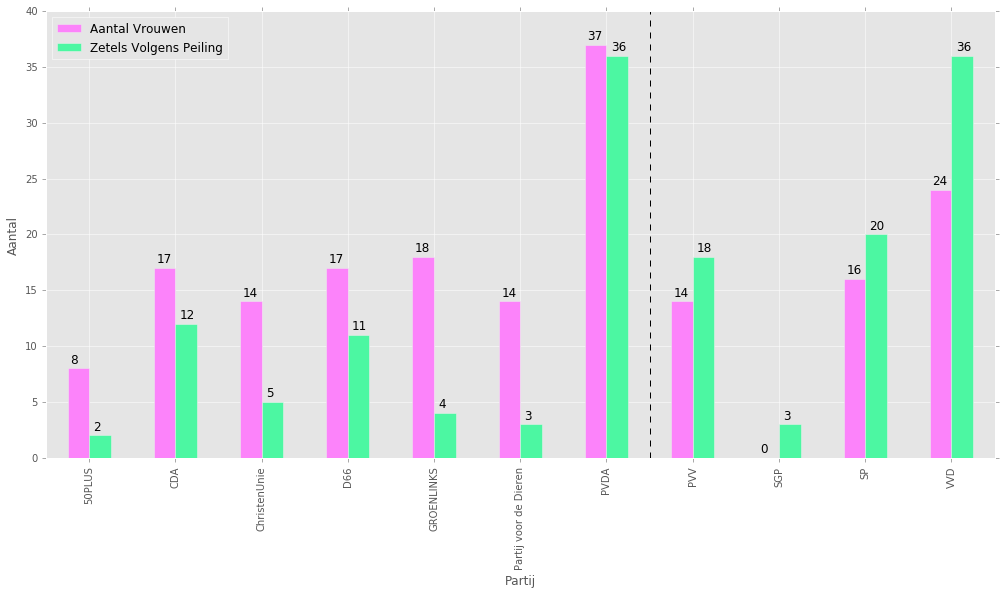
\includegraphics[width=\linewidth]	{Aantal_vrouwen_aantal_zetels1.png}

			\caption{Het aantal vrouwen (paarse staven) op de kandidatenlijst \citep{Kiesraad_kandidatenlijsten} en het aantal zetels (groene staven) volgens de peilingen per partij \citep{IPSOS}.}

	\label{fig:zetelsV}
\end{figure}

\paragraph{Maximaal aantal vrouwen per partij (top \textit{N}) dat in de Tweede Kamer gekozen had kunnen worden.}
In Figuur \ref{fig:zetelsV} is te zien hoeveel zetels een partij zou gaan ontvangen volgens de peiling en hoeveel vrouwelijke kandidaten de partij op de kandidatenlijst had staan. In tabel \ref{table:topNV} is daaruit voortvloeiend te zien hoeveel vrouwelijke kandidaten er per partij maximaal in de Tweede Kamer gekozen hadden kunnen worden.  


\begin{table}[h]
\centering
	\begin{footnotesize}
		\begin{tabular}{lrr}
\toprule
{} &  Top \textit{N} Vrouwelijke Kandidaten  &  Overgebleven Mannelijke Kandidaten  \\
Partij                &        &        \\
\midrule
50PLUS                &                              2 &       0 \\
CDA                   &                             12 &       0 \\
ChristenUnie          &                              5 &       0 \\
D66                   &                             11 &       0 \\
GROENLINKS            &                              4 &       0 \\
Partij v d Dieren &                              3 &       0 \\
PVDA                  &                             36 &       0 \\
PVV                   &                             14 &       4 \\
SGP                   &                              0 &       3 \\
SP                    &                             16 &       4 \\
VVD                   &                             24 &      12 \\
\midrule
Totaal                &                            127 &      23 \\
\bottomrule
\end{tabular}

	\end{footnotesize}
			\caption{Per partij de top \textit{N} vrouwelijke kandidaten en de overgebleven mannelijke kandidaten a.d.h.v. de peiling \citep{IPSOS}.}
\label{table:topNV} 
\end{table}

De SGP had helemaal geen vrouwelijke kandidaten op de kandidatenlijst staan en de PVV, de SP en de VVD zouden volgens de peiling meer zetels gaan ontvangen dan dat zij vrouwelijke kandidaten op de kandidatenlijsten hadden staan. Zodoende komt het totaal aantal vrouwelijke kandidaten dat volgens de peiling in de Tweede Kamer gekozen had kunnen worden uit op 127. De overgebleven 23 kandidaten die op basis van de peiling in de Tweede Kamer gekozen zouden worden, zijn uiteraard mannelijke kandidaten.

\paragraph{Het toewijzen van de stemmen aan de vrouwelijke kandidaten op basis van de peiling.}
Zoals te zien in Tabel \ref{table:tab1V}, hebben we berekend hoeveel stemmen een partij, volgens de peiling, werd verwacht te gaan ontvangen en hoeveel stemmen van vrouwelijke kiezers een partij verwacht werd te gaan ontvangen. Nu gaan we deze vrouwelijke stemmen toewijzen aan vrouwelijke kandidaten op de kandidatenlijsten. De reden hiervoor is dat er zodoende een voorspelling gedaan kan worden over het aantal stemmen dat de top \textit{N} vrouwelijke kandidaten van een partij per vrouwelijke kandidaat zou hebben kunnen verwachten. Ter illustratie nemen we weer de PVDA als voorbeeld.

Voor de PVDA werd verwacht dat zij een totaal aantal van 1.111.627 vrouwelijke stemmen zouden gaan ontvangen. Deze stemmen worden verdeeld over de top \textit{N} vrouwelijke kandidaten van de PVDA. Zoals eerder al vastgesteld, en te zien in Tabel \ref{table:topNV}, heeft de PVDA een $N=36$. De stemmen van vrouwelijke kiezers op de PVDA worden willekeurig (gelijk) verdeeld over de eerste 36 vrouwelijke kandidaten op de kandidatenlijst van de PVDA. Daarmee zouden de top 36 vrouwelijke kandidaten van de PVDA (ongeveer) het aantal van ($1.111.627\div36$ = ) 30.878 stemmen per kandidaat hebben ontvangen. Dat is ruim boven de verwachte voorkeursdrempel van het aantal van 15.439 stemmen. In de grafiek in Figuur \ref{fig:stemmenV1} is, gebaseerd op de peiling, de verdeling van vrouwelijke stemmen op vrouwelijke kandidaten voor alle partijen te zien.

Zoals te zien in Figuur \ref{fig:stemmenV1}, kan volgens de peiling voor alle top \textit{N} vrouwelijke kandidaten verwacht worden dat zij boven de verwachte voorkeursdrempel uitkomen. Hierdoor zou het mogelijk zijn geweest dat alle 127 top \textit{N} vrouwelijke kandidaten in de Tweede Kamer gestemd konden worden. Wat opvalt is dat voor zeven verschillende partijen het aantal te verwachte stemmen op een vrouwelijke kandidaat van de partijen exact hetzelfde is. Dit is geen toeval maar ligt ten grondslag aan de manier van berekenen.

  
\begin{figure}[H]

	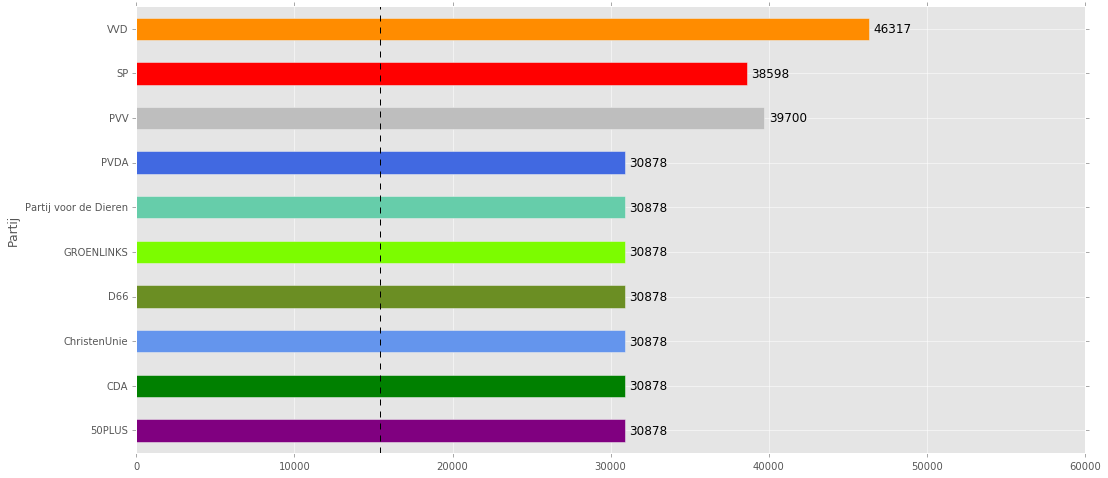
\includegraphics[width=\linewidth]	{stemmen_op_vrouwen_topN_peiling.png}

			\caption{Grafiek met per partij met vrouwelijke kandidaten, de verdeling van de stemmen van vrouwelijk kiezers op de top \textit{N} vrouwelijke kandidaten aan de hand van de peiling \citep{IPSOS}. De stippellijn is de verwachte voorkeursdrempel(15.439 stemmen).}

\label{fig:stemmenV1}
\end{figure}


De partijen waarbij het aantal stemmen op een top \textit{N} vrouwelijke kandidaat hetzelfde zou zijn geweest, hebben allemaal één ding gemeen: de top \textit{N} is gelijk aan het aantal te verwachten zetels. Zoals eerder al is uitgelegd, is het aantal stemmen dat nodig is voor één te verwachten zetel gelijk aan de verwachte kiesdeler (61.757 stemmen). Vanwege de aanname dat 50\% van de stemmen op een partij van vrouwelijke kiezers zal komen, wordt de kiesdeler vermenigvuldigd met 50\%. In het geval dat een partij bijvoorbeeld één zetel verwachtte te gaan ontvangen, is het aantal stemmen dat voor deze partij werd verwacht gelijk aan de verwachte kiesdeler. Wanneer 50\% van de stemmen van vrouwelijk kiezers zou zijn gekomen en van deze kiezers verwacht werd dat zij allemaal op de enige mogelijke vrouwelijke kandidaat zouden hebben gestemd (voor deze partij geldt dan $N=1$), zou deze vrouwelijke kandidaat het verwachte aantal van ($50\%*61.757$ = ) 30.878 stemmen hebben ontvangen. 


\paragraph{Het toewijzen van de stemmen aan de vrouwelijke kandidaten op basis van einduitslag.}
In de vorige paragraaf werd uitgelegd hoe we, aan de hand van de peiling, een voorspelling konden gaan doen over het aantal stemmen dat een top \textit{N} vrouwelijke kandidaat kon gaan verwachten. Zoals te zien in Tabel \ref{table:tab2V} en zoals we eerder in dit hoofdstuk hebben berekend, weten we hoeveel stemmen van vrouwelijke kiezers een partij volgens de einduitslag had ontvangen. Zodoende kunnen we het aantal stemmen van vrouwelijke kiezers gaan toewijzen aan de vrouwelijke kandidaten en kunnen we daarmee gaan bepalen of de voorspelling uit de vorige paragraaf enigszins correct zou zijn geweest. Ter illustratie nemen we weer de PVDA als voorbeeld. 

De PVDA had bij de einduitslag een totaal aantal van 1.217.190 vrouwelijke stemmen ontvangen. Deze stemmen worden willekeurig verdeeld over de top 36 (voor de PVDA geldt $N=36$) vrouwelijke kandidaten op de kandidatenlijst van de PVDA. Daarmee zouden de deze vrouwelijke kandidaten het aantal van ($1.217.190\div36$ = ) 33.810 stemmen per kandidaat hebben ontvangen. Dat is ruim boven de daadwerkelijke voorkeursdrempel van 15.708 stemmen. In de grafiek in Figuur \ref{fig:stemmenV2} is, gebaseerd op de einduitslag, de verdeling van vrouwelijke stemmen op vrouwelijke kandidaten voor alle partijen te zien.

  
\begin{figure}[H]

	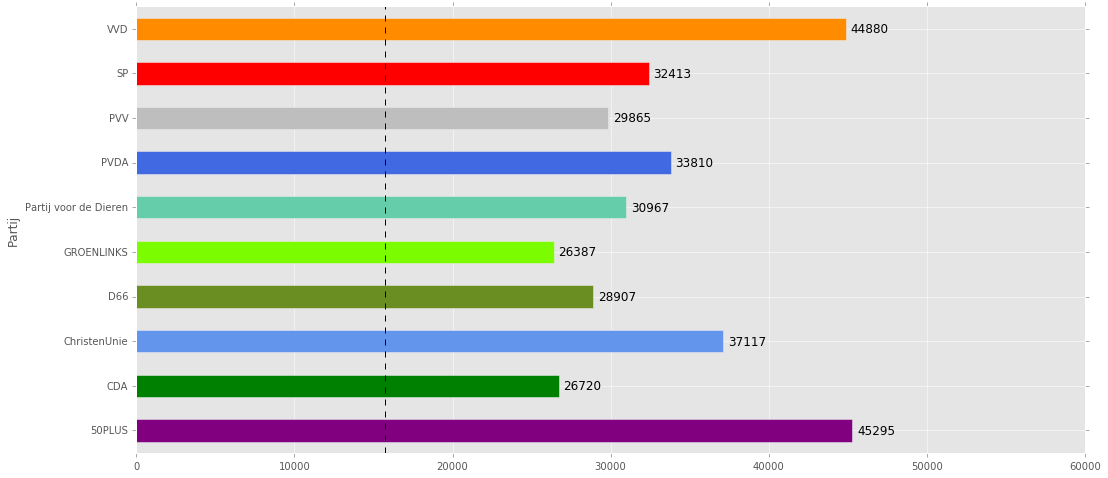
\includegraphics[width=\linewidth]	{stemmen_op_vrouwen_topN_uitslag.png}

			\caption{Grafiek met per partij de verdeling van de stemmen van vrouwelijk kiezers op de top \textit{N} vrouwelijke kandidaten aan de hand van de einduitslag \citep{Kiesraad_databank}. De SGP wordt niet in de grafiek getoond omdat deze partij geen vrouwelijke kandidaten op de kandidatenlijst had staan. De stippellijn is de daadwerkelijke voorkeursdrempel (15.708 stemmen).}

\label{fig:stemmenV2}
\end{figure}

Zoals te zien in Figuur \ref{fig:stemmenV2} hierboven, zouden alle top \textit{N} vrouwelijke kandidaten van de partijen boven de daadwerkelijke voorkeursdrempel uitgekomen zijn. Ofschoon de precieze aantallen niet exact hetzelfde zijn, is de voorspelling uit de vorige paragraaf correct in het feit dat de top \textit{N} vrouwelijke kandidaten van alle partijen boven de voorkeursdrempel uitgekomen zouden zijn. Het zou op basis van de einduitslag nog altijd mogelijk zijn geweest dat er 127 vrouwelijke kandidaten in de Tweede Kamer gekozen zouden worden wanneer de strategie zou zijn uitgevoerd. 

\paragraph{Aantal vrouwen na strategie 1.}
Na het uitvoeren van de strategie 1 en het opstellen van de Tweede Kamer zoals eerder in dit hoofdstuk beschreven (zie Paragraaf \hyperref[opstellen]{Het uiteindelijk opstellen van de Tweede Kamer na uitvoering van een strategie.}), zou strategie 1 een Tweede Kamer hebben opgeleverd waarin 121 vrouwen en 29 mannen plaats zouden hebben genomen. Daarmee zouden vrouwen (met 81\%) ruim in hogere mate vertegenwoordigd zijn geweest dan mannen (met 19\%). In de cirkeldiagram in Figuur \ref{fig:pcS1V} hieronder is de verdeling goed te zien. In de volgende paragraaf wordt uitgelegd waarom er niet 127 maar 'slechts' 121 vrouwen in de Tweede Kamer plaats zouden nemen na uitvoering van strategie 1.

\begin{figure}[H]
\centering
	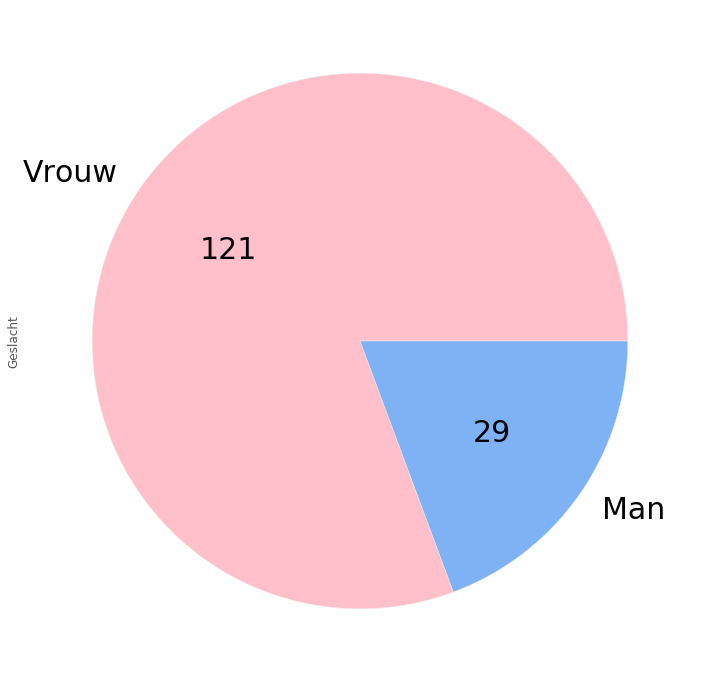
\includegraphics[width=0.35\linewidth]{pie_chart_topN.png}

			\caption{Na uitvoering van de strategie nemen er 121 vrouwen (81\%) en 29 mannen (19\%) plaats in de Tweede Kamer.}

\label{fig:pcS1V}
\end{figure}

\newpage
\paragraph{Minder dan 127 vrouwen in de Tweede Kamer na uitvoering van strategie 1.}
De reden dat er niet 127 vrouwen maar 'slechts' 121 vrouwen in de Tweede Kamer zouden hebben plaatsgenomen na uitvoering van strategie 1 ligt ten grondslag aan een aantal factoren. Zo hadden het merendeel van de partijen die zetels ontvingen een mannelijke kandidaat als lijsttrekker en ontvingen deze lijsttrekkers de meeste stemmen in vergelijking met alle andere kandidaten van dezelfde partij. Hierdoor zou er bij de 50PLUS, de ChristenUnie en de SP één vrouwelijke kandidaat af zijn gevallen. Daarnaast had de SP minder zetels behaald bij de einduitslag dan dat zij volgens de peiling zouden gaan ontvangen. Hierdoor zou ook bij de SP nog een vrouwelijke kandidaat af zijn gevallen. Ook de Partij voor de Dieren ontving minder zetels bij de einduitslag dan zij volgens de peiling zouden gaan ontvangen en, ondanks het feit dat zij een vrouwelijke lijsttrekker hadden in de persoon van Marianne Thieme, zou dit geresulteerd hebben in één afgevallen vrouwelijke kandidaat. Bij het CDA had een mannelijke kandidaat in de persoon van Pieter Omtzigt meer stemmen ontvangen dan de vrouwelijke kandidaten zouden hebben ontvangen. Hierdoor viel bij het CDA een vrouwelijke kandidaat af. Dit komt op een totaal van zes afgevallen vrouwelijke kandidaten, oftewel een totaal van ($127-6$ = ) 121 vrouwen in de Tweede Kamer na uitvoering van strategie 1.  



\subsubsection{Strategie 2: Vrouwelijke kiezers stemmen op een willekeurig vrouwelijke kandidaat.}
\paragraph{Regels.}
\begin{itemize}
	\item
Het aantal stemmen van vrouwelijke kiezers die een partij krijgt, worden volstrekt willekeurig verdeeld over alle vrouwelijke kandidaten die op de kandidatenlijst staan van de partij. Hierbij is de \textit{N} per partij het totaal aantal vrouwelijke kandidaten die de partij op de kandidatenlijst heeft staan. 	\\ 	
\end{itemize}	

\paragraph{Het toewijzen van de stemmen aan de vrouwelijke kandidaten op basis van de peiling en de einduitslag.}
Zoals we bij de vorige strategie hebben gedaan, zullen we ook voor strategie 2 de stemmen toewijzen om aan de hand van de peiling een voorspelling te kunnen doen betreffende het aantal te stemmen die per vrouwelijke kandidaat verwacht had kunnen worden. Om te kijken of de voorspelling enigszins correct zou zijn geweest en om te weten van welke partijen de vrouwelijke kandidaten boven de daadwerkelijke voorkeursdrempel uitgekomen zouden zijn geweest, zullen we ook de stemmen op vrouwelijke kandidaten op basis van de einduitslag toewijzen. In Figuur \ref{fig:stemmenS2V} op de volgende pagina is zowel de toewijzing op basis van de peiling (licht gekleurde staven) alsmede de toewijzing op basis van de einduitslag (donker gekleurde staven) te zien. Ten behoeve van de leesbaarheid zijn deze toewijzingen in één grafiek samengebracht.  

Zoals te zien in Figuur \ref{fig:stemmenS2V} op de volgende pagina, zouden zowel volgens de peiling (voorspelling) alsmede volgens de einduitslag niet alle vrouwelijke kandidaten van de partijen boven de daadwerkelijke voorkeursdrempel uitgekomen zijn. Ofschoon de precieze aantallen niet exact hetzelfde zijn, is met strategie 2 de voorspelling zoals berekend a.d.h.v. de peiling correct in het voorspellen welke partijen met alle vrouwelijke kandidaten boven de voorkeursdrempel uitgekomen zouden zijn en bij welke partijen dit niet het geval geweest zou zijn.


\begin{figure}[H]

	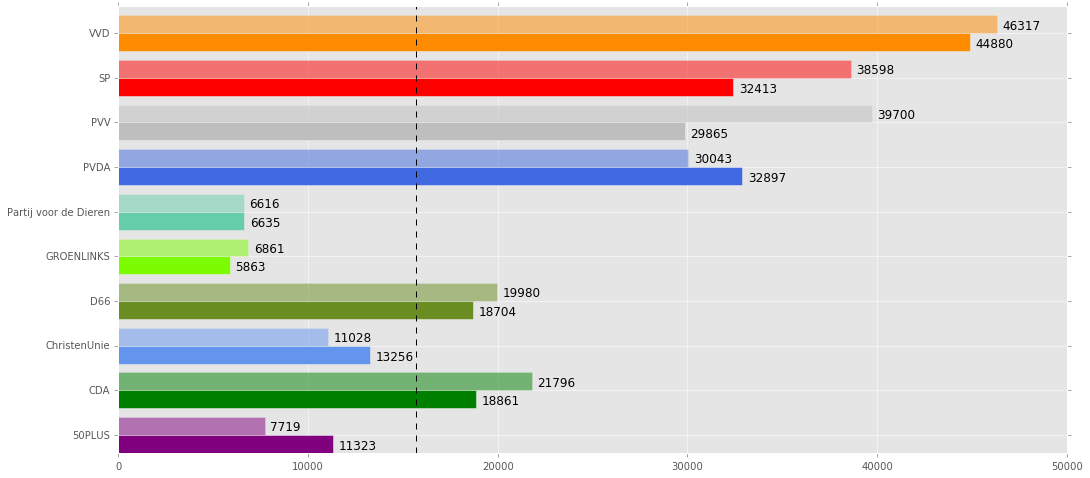
\includegraphics[width=\linewidth]	{stemmen_op_vrouwen_willekeurig_samen.png}

			\caption{Grafiek met per partij de verdeling van de stemmen van vrouwelijk kiezers op alle vrouwelijke kandidaten van de partij a.d.h.v. de peiling \citep{IPSOS} in de licht gekleurd staven en a.d.h.v. de einduitslag \citep{Kiesraad_databank} in de donker gekleurde staven. De stippellijn is de daadwerkelijk voorkeursdrempel(15.708 stemmen).}

\label{fig:stemmenS2V}
\end{figure}


\paragraph{Aantal vrouwen na strategie 2.}
Na het uitvoeren van strategie 2 en het opstellen van de Tweede Kamer zoals eerder in dit hoofdstuk beschreven, zou strategie 2 uiteindelijk een Tweede Kamer hebben opgeleverd waarin 116 vrouwen en 34 mannen zouden hebben plaatsgenomen. Daarmee zouden vrouwen (met 77\%) ruim in hogere mate vertegenwoordigd zijn geweest dan mannen(met 23\%). In de cirkeldiagram in Figuur \ref{fig:pcS2V} hieronder is de verdeling goed te zien. In de volgende paragraaf wordt uitgelegd waarom er niet 121 (zoals in de vorige strategie) maar 'slechts' 116 vrouwen in de Tweede Kamer plaats zouden hebben genomen na uitvoering van strategie 2 ten opzichte van uitvoering van strategie 1.

\begin{figure}[H]
\centering
	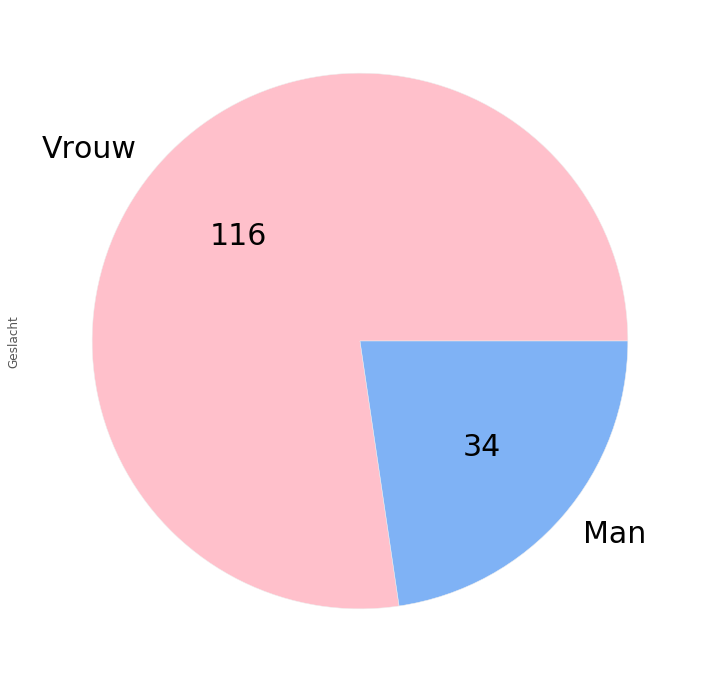
\includegraphics[width=0.35\linewidth]{pie_chart_willekeurig.png}

			\caption{Na uitvoering van de strategie nemen er 116 vrouwen (77\%) en 34 mannen (23\%) plaats in de Tweede Kamer.}

\label{fig:pcS2V}
\end{figure}

\paragraph{Minder vrouwen in de Tweede Kamer d.m.v. uitvoering van strategie 2 dan d.m.v. uitvoering van strategie 1.}
De reden dat er, na uitvoering van strategie 2, 116 vrouwen in de Tweede Kamer plaats zouden hebben genomen en dat vijf vrouwen minder zijn dan bij uitvoering van strategie 1 ligt ten grondslag aan het feit dat de vrouwelijke kandidaten van de Partij voor de Dieren, GROENLINKS, de ChristenUnie en 50PLUS minder stemmen zouden hebben ontvangen dan het aantal stemmen van de voorkeursdrempel. Bij de Partij voor de Dieren zou dit echter geen negatief effect hebben gehad vanwege het feit dat de partij twee zetels ontving en de eerste twee plaatsen op de kandidatenlijst bezet werden door vrouwelijke kandidaten. Bij zowel GROENLINKS alsmede de ChristenUnie zouden er echter twee vrouwelijke kandidaten af zijn gevallen. Bij 50PLUS zou er één vrouwelijke kandidaat af zijn gevallen. Geen enkele partij zou meer vrouwen in de Tweede Kamer hebben gekregen na uitvoering van strategie 2 ten opzichte van uitvoering van strategie 1.   


\subsubsection{Strategie 3.1: Vrouwelijke kiezers stemmen willekeurige op één van de eerste 15 vrouwelijke kandidaten van een partij.}

\paragraph{Regels.}
\begin{itemize}
\item
Elke partij krijgt een eigen \textit{N}:
	\begin{itemize}
		\item
Wanneer een partij minstens vijftien vrouwelijke kandidaten op de kandidatenlijst heeft staan geldt voor de partij $N=15$.
		\item
Wanneer een partij minder dan 15 vrouwelijke kandidaten op de kandidatenlijst heeft staan, geldt voor de partij $N=$ het totaal aantal vrouwelijke kandidaten wat de partij op de kandidatenlijst heeft staan.\\
	\end{itemize}
\end{itemize}

\paragraph{Partijen met minstens 15 vrouwelijke kandidaten en partijen met minder dan 15 vrouwelijke kandidaten.}
Hieronder is in de grafiek in Figuur \ref{fig:15V} per partij te zien of de partij voldeed aan de drempel van minstens 15 vrouwelijke kandidaten op de kandidatenlijst om de zodoende de vrouwelijke stemmen op de partij te verdelen over de top 15 vrouwelijke kandidaten van de partij. We zien dat bij D66, GROENLINKS, de PVDA, het CDA, de SP en de VVD de stemmen van vrouwelijke kiezers over de top 15 vrouwelijke kandidaten verdeeld hadden kunnen worden. Bij de Partij voor de Dieren, de ChristenUnie, 50PLUS en de PVV zouden de stemmen van vrouwelijke kiezers die de partij volgens de peiling zou gaan ontvangen verdeeld hebben moeten worden over alle vrouwelijke kandidaten die deze partijen op hun kandidatenlijst hadden staan.

\begin{figure}[H]

	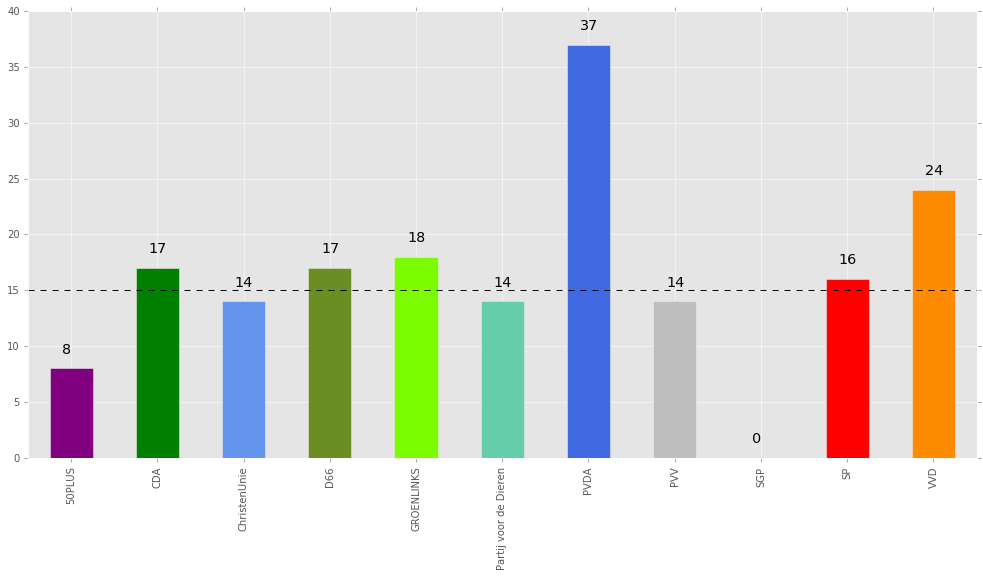
\includegraphics[width=\linewidth]	{top15_of_topN_kandidaten.png}

			\caption{De grafiek toont bij welke partijen de vrouwelijke kiezers op de top 15 vrouwelijke kandidaten \citep{Kiesraad_kandidatenlijsten} van de partij kunnen gaan stemmen ($N=15$) en van welke partijen de vrouwelijke kiezers op alle vrouwelijke kandidaten van de partij kunnen gaan stemmen (\textit{N}=\textit{totaal aantal vrouwelijke kandidaten}).}  

\label{fig:15V}
\end{figure}

\paragraph{Het toewijzen van de stemmen aan de vrouwelijke kandidaten op basis van de peiling en de einduitslag.}
Zoals te zien in Tabel \ref{table:tab1V}, hebben we berekend hoeveel stemmen een partij, volgens de peiling, verwacht werd te gaan ontvangen en hoeveel stemmen van vrouwelijke kiezers een partij verwacht werd te gaan ontvangen. Nu gaan we de vrouwelijke stemmen toewijzen aan vrouwelijke kandidaten op de kandidatenlijsten. 

Op dezelfde wijze als we bij de vorige strategie hebben gehanteerd zullen we ook voor strategie 3 de stemmen toewijzen om a.d.h.v. de peiling een voorspelling te kunnen doen betreffende het aantal stemmen dat per vrouwelijke kandidaat verwacht had kunnen worden. Om de voorspelling te evalueren en om te weten van welke partijen de top \textit{N} vrouwelijke kandidaten boven de voorkeursdrempel uitgekomen zouden zijn, zullen we ook de stemmen op vrouwelijke kandidaten op basis van de einduitslag toewijzen. In Figuur \ref{fig:stemmenS31V} hieronder is zowel de toewijzing op basis van de peiling alsmede de toewijzing op basis van de einduitslag te zien.  



\begin{figure}[H]

	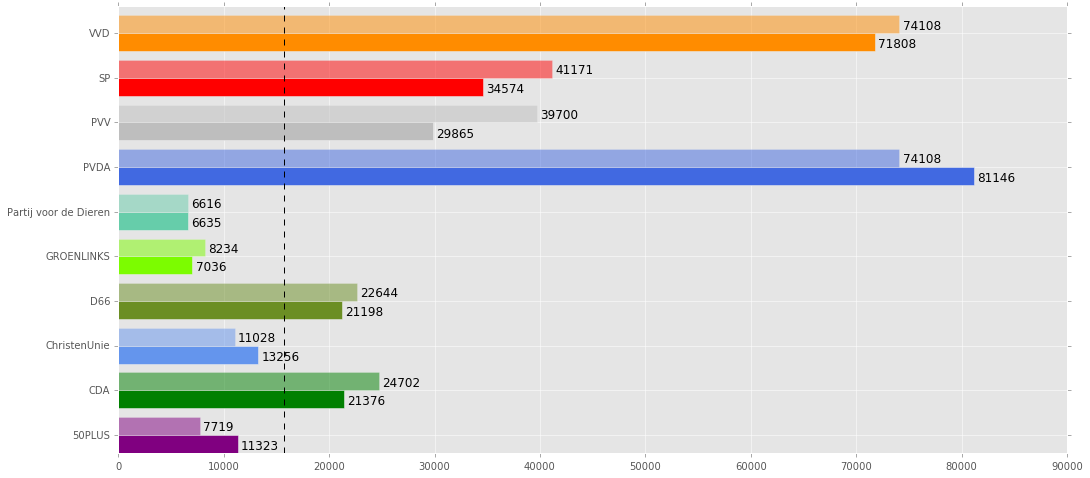
\includegraphics[width=\linewidth]	{stemmen_op_vrouwen_top15_of_topN_samen.png}

			\caption{Grafiek met per partij de verdeling van de stemmen van vrouwelijk kiezers op de top 15 vrouwelijke kandidaten van de partij a.d.h.v. de peiling \citep{IPSOS} in de licht gekleurd staven en a.d.h.v. de einduitslag \citep{Kiesraad_databank} in de donker gekleurde staven. De stippellijn is de daadwerkelijk voorkeursdrempel(15.708 stemmen).} 

\label{fig:stemmenS31V}
\end{figure}

In Figuur \ref{fig:stemmenS31V} hierboven is te zien dat zowel volgens de peiling (voorspelling) alsmede volgens de einduitslag niet alle top \textit{N} vrouwelijke kandidaten van de partijen boven de daadwerkelijke voorkeursdrempel zouden zijn uitgekomen. Ofschoon de precieze aantallen niet exact hetzelfde zijn, is ook met strategie 3 de voorspelling zoals berekend a.d.h.v. de peiling correct in het voorspellen welke partijen met de top \textit{N} ($N=15$ of $N=$totaal aantal vrouwelijke kandidaten) vrouwelijke kandidaten boven de voorkeursdrempel uitgekomen zouden en bij welke partijen dit niet het geval geweest zou zijn.


\paragraph{Aantal vrouwen na strategie 3.1.}
Na het uitvoeren van de strategie 3.1 en het opstellen van de Tweede Kamer zoals eerder in dit hoofdstuk beschreven, zou strategie 3.1 uiteindelijk een Tweede Kamer hebben opgeleverd waarin 91 vrouwen en 59 mannen zouden hebben plaatsgenomen. Daarmee zouden vrouwen (met 61\%) in hogere mate vertegenwoordigd zijn geweest dan mannen (met 39\%). In de cirkeldiagram in Figuur \ref{fig:pcS31V} op de volgende pagina is de verdeling goed te zien. In de volgende paragraaf wordt uitgelegd waarom er niet 116 (zoals met de vorige strategie) maar slechts 91 vrouwen in de Tweede Kamer plaats zouden hebben genomen na uitvoering van strategie 3.1 ten opzichte van uitvoering van strategie 2.

\begin{figure}[H]
\centering
	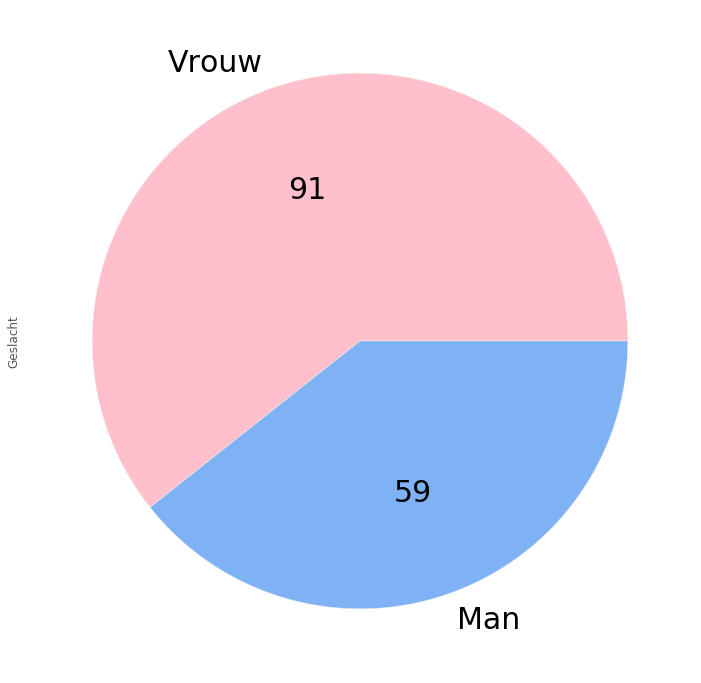
\includegraphics[width=0.35\linewidth]{pie_chart_top15_of_topN.png}

			\caption{Na uitvoering van de strategie nemen er 91 vrouwen (61\%) en 59 mannen (39\%) plaats in de Tweede Kamer.}

\label{fig:pcS31V}
\end{figure}

\paragraph{Minder vrouwen in de Tweede Kamer d.m.v. uitvoering van strategie 3.1 dan d.m.v. uitvoering van strategie 2.}
De reden dat er, na uitvoering van strategie 3.1, 91 vrouwen in de Tweede Kamer zouden hebben genomen en dat er daarmee 25 vrouwen minder in de Tweede Kamer zouden hebben plaatsgenomen dan bij strategie 2 het geval zou zijn geweest, ligt ten grondslag aan het feit dat er bij de VVD acht vrouwelijke kandidaten zouden zijn afgevallen ten opzichte van strategie 2. Dit komt omdat de stemmen niet verdeeld zouden zijn over alle 24 vrouwelijke kandidaten van de VVD maar over de top 15 vrouwelijke kandidaten van de VVD. De top 15 vrouwelijke kandidaten van de VVD zouden daardoor allen een zetel hebben ontvangen in de Tweede Kamer. Daarnaast zou ook een 16e vrouwelijke kandidaat, in de persoon van Ingrid de Caluwé, een zetel in de Tweede Kamer hebben ontvangen vanwege haar plaats op de kandidatenlijst. Bij de PVDA zouden er zeventien vrouwelijke kandidaten zijn afgevallen ten opzichte van strategie 2. Dit komt ook hier door het feit dat de vrouwelijke stemmen over de top 15 vrouwelijke kandidaten verdeeld zouden zijn geweest. Daarnaast ontvingen vier vrouwelijke kandidaten van de PVDA een zetel in de Tweede Kamer vanwege hun plaats op de kandidatenlijst. In totaal zouden er dus 25 (zeventien van de PVDA en acht van de VVD) vrouwen buiten de boot vallen na uitvoering van strategie 3.1 ten opzichte van uitvoering van  strategie 2. Daarmee zou het totale aantal vrouwen in de Tweede Kamer uitgekomen zijn op ($116-25$ = ) 91. 



\subsubsection{Strategie 3.2: Vrouwelijke kiezers stemmen willekeurige op één van de eerste \textit{N} vrouwelijke kandidaten van een partij.}

\paragraph{Regels.}
\begin{itemize}
\item
Elke partij krijgt een eigen \textit{N}:

	\begin{itemize}
		\item
Wanneer een partij minder dan 10 vrouwelijke kandidaten op de kandidatenlijst heeft staan geldt voor de partij $N=5$.
		\item
Wanneer een partij tien of meer maar minder dan vijftien vrouwelijke kandidaten op de kandidatenlijst heeft staan geldt voor de partij $N=10$.
		\item
Wanneer een partij vijftien of meer maar minder dan dertig vrouwelijke kandidaten op de kandidatenlijst heeft staan geldt voor de partij $N=15$.
		\item
Wanneer een partij dertig of meer vrouwelijke kandidaten op de kandidatenlijst heeft staan geldt voor de partij $N=30$.
	\end{itemize}
\end{itemize}


\paragraph{Voor elke partij de eigen \textit{N} bepalen.}
Hieronder is in de grafiek in Figuur \ref{fig:XV} per partij te zien op welke waarde de \textit{N} aantal vrouwelijke kandidaten wordt bepaald. De SGP had geen vrouwelijke kandidaten op de kandidaten lijst dus de SGP krijgt geen eigen \textit{N}. 50PLUS had minder dan tien vrouwelijke kandidaten op de kandidatenlijst en daardoor geldt voor 50PLUS $N=5$. De ChristenUnie, de Partij voor de Dieren en de PVV hadden tien of meer vrouwelijke kandidaten op de kandidatenlijst staan maar minder dan 15. Hierdoor geldt voor deze partijen $N=10$. Het CDA, D66, GROENLINKS, de SP en de VVD hebben vijftien of meer vrouwelijke kandidaten op de kandidatenlijsten maar minder dan dertig. Hierdoor geldt voor deze partijen $N=15$. Enkel de PVDA heeft meer dan dertig vrouwelijke kandidaten op de kandidatenlijst staan en daardoor geldt voor de PVDA $N=30$.

\begin{figure}[H]

	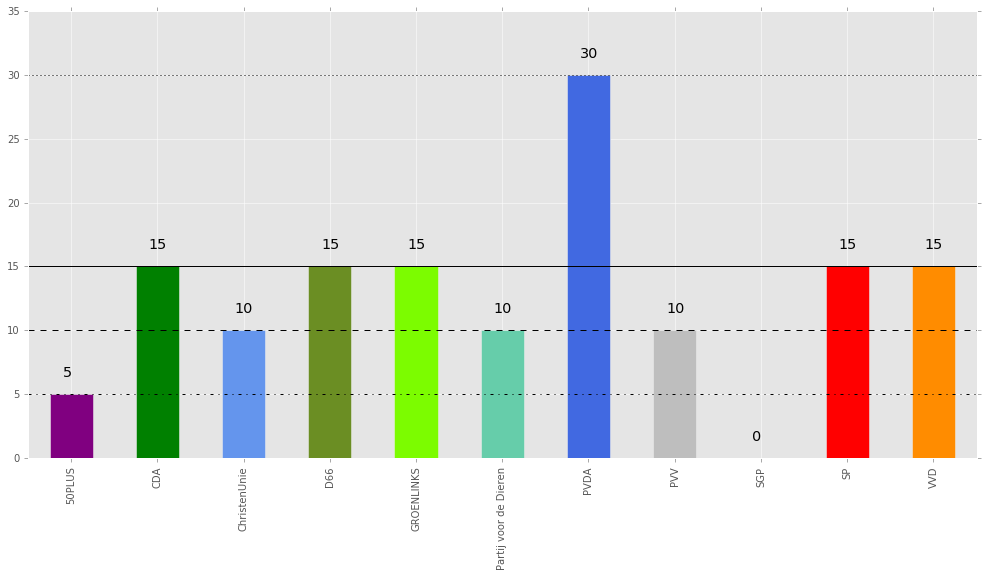
\includegraphics[width=\linewidth]{eigenX_partijen.png}

			\caption{Elke partij krijgt, afhankelijke van het aantal vrouwelijke kandidaten op de kandidatenlijst, een eigen \textit{N}. De lijnen geven een verschillende mogelijke \textit{N} aan.}

\label{fig:XV}
\end{figure}

\paragraph{Het toewijzen van de stemmen aan de vrouwelijke kandidaten op basis van de peiling en de einduitslag.}
Zoals te zien in Tabel \ref{table:tab1V} hebben we berekend hoeveel stemmen een partij volgens de peiling verwacht werd te gaan ontvangen en hoeveel stemmen van vrouwelijke kiezers een partij verwacht werd te gaan ontvangen. Nu gaan we de vrouwelijke stemmen toewijzen aan vrouwelijke kandidaten op de kandidatenlijsten. Op dezelfde wijze als bij de voorgaande strategie\"{e}n is gehanteerd zullen we ook voor strategie 3.2 de stemmen toewijzen om a.d.h.v. de peiling een voorspelling te kunnen doen betreffende het aantal stemmen dat per vrouwelijke kandidaat verwacht had kunnen worden. Om de voorspelling te evalueren en om te weten van welke partijen de top \textit{N} vrouwelijke kandidaten boven de voorkeursdrempel uitgekomen zouden zijn geweest, zullen we ook de stemmen op vrouwelijke kandidaten op basis van de einduitslag toewijzen. In Figuur \ref{fig:stemmenS32V} op de volgende pagina is zowel de toewijzing op basis van de peiling alsmede de toewijzing op basis van de einduitslag te zien.  




\begin{figure}[h]

	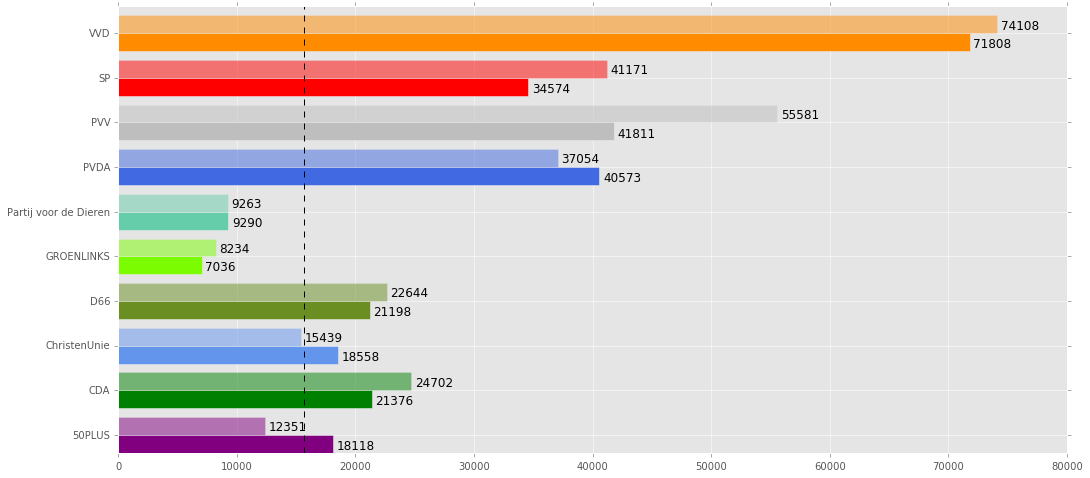
\includegraphics[width=\linewidth]{stemmen_op_vrouwen_eigenX_samen.png}

			\caption{Grafiek met per partij de verdeling van de stemmen van vrouwelijk kiezers op de top \textit{N} vrouwelijke kandidaten van de partij a.d.h.v. de peiling \citep{IPSOS} in de licht gekleurd staven en a.d.h.v. de einduitslag \citep{Kiesraad_databank} in de donker gekleurde staven. De stippellijn is de daadwerkelijk voorkeursdrempel(15.708 stemmen).}

\label{fig:stemmenS32V}
\end{figure}


In Figuur \ref{fig:stemmenS32V} op de volgende pagina is te zien dat zowel volgens de peiling (voorspelling) alsmede volgens de einduitslag niet alle top \textit{N} vrouwelijke kandidaten van de partijen boven de daadwerkelijke voorkeursdrempel zouden zijn uitgekomen. Ofschoon de precieze aantallen niet exact hetzelfde zijn, is met strategie 3.2 de voorspelling zoals berekend a.d.h.v. de peiling grotendeels correct in het voorspellen welke partijen met de top \textit{N} vrouwelijke kandidaten boven de voorkeursdrempel zouden zijn uitgekomen en bij welke partijen dit niet het geval geweest zou zijn. Echter is er voor de ChristenUnie voorspeld dat de top tien vrouwelijke kandidaten (voor ChristenUnie geldt $N=10$) boven de voorkeursdrempel uitgekomen zouden zijn komen terwijl dit bij de einduitslag niet het geval zou zijn geweest. Dit ligt ten grondslag aan het feit dat de ChristenUnie een kleiner aantal stemmen kreeg dan de peiling had voorspeld. 

\paragraph{Aantal vrouwen na strategie 3.2.}
Na het uitvoeren van de strategie 3.2 en het opstellen van de Tweede Kamer zoals eerder in dit hoofdstuk is beschreven, zou strategie 3.2 uiteindelijk een Tweede Kamer hebben opgeleverd waarin 101 vrouwen en 49 mannen zouden hebben plaatsgenomen. Daarmee zouden vrouwen (met 67\%) in hogere mate vertegenwoordigd zijn geweest dan mannen(met 33\%). In de cirkeldiagram in Figuur \ref{fig:pcS32V} hieronder is de verdeling goed te zien. In de volgende paragraaf wordt uitgelegd waarom er een toename is van 91 naar 101 vrouwen die in de Tweede Kamer zouden hebben plaatsgenomen na uitvoering van strategie 3.2 ten opzichte van uitvoering van strategie 3.1.

\begin{figure}[H]
\centering
	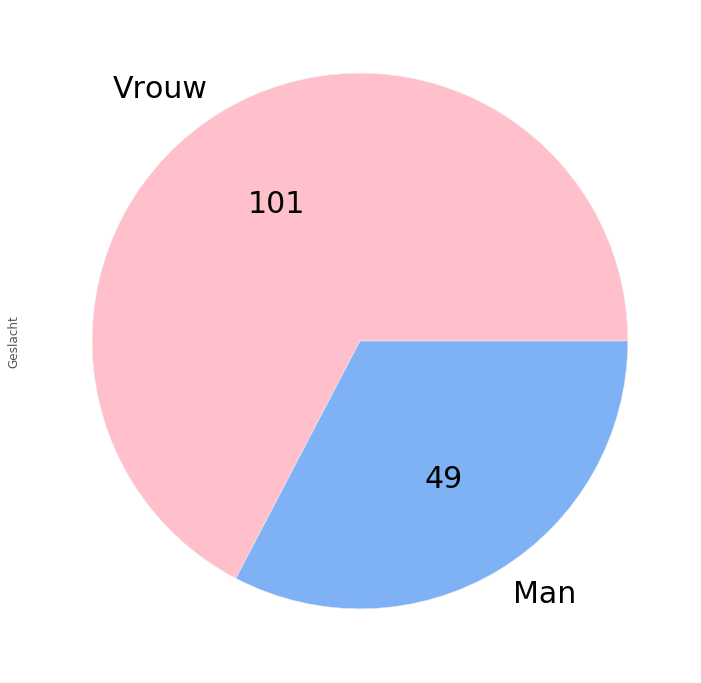
\includegraphics[width=0.35\linewidth]{pie_chart_eigenX.png}

			\caption{Na uitvoering van de strategie nemen er 101 vrouwen(67\%) en 49 mannen(33\%) plaats in de Tweede Kamer.}

\label{fig:pcS32V}
\end{figure}

\paragraph{Meer vrouwen in de Tweede Kamer d.m.v. uitvoering van strategie 3.2 dan d.m.v. uitvoering van strategie 3.1.}
De reden dat er, na uitvoering van strategie 3.1, 101 vrouwen in de Tweede Kamer plaats zouden hebben genomen en dat er daarmee tien vrouwen meer in de Tweede Kamer zouden zijn geweest ten opzichte van strategie 3.1 ligt ten grondslag aan het feit 50PLUS één vrouwelijke kandidaat meer in de Tweede Kamer zou krijgen dan bij de strategie 3.1. 
De ChristenUnie zou twee vrouwelijke kandidaten in de Tweede Kamer erbij hebben gekregen ten opzichte van strategie 3.1. De PVDA zou elf vrouwelijke kandidaten erbij hebben gekregen ten opzichte van strategie 3.1. Tot slot zouden er vier vrouwelijke kandidaten bij de PVV af zijn gevallen. Dit komt omdat de vrouwelijke stemmen niet meer verdeeld zouden worden over de veertien vrouwelijke kandidaten die op de kandidatenlijst van de PVV stonden, maar over de top 10 (de eerder vastgestelde top \textit{N} van de PVV) vrouwelijke kandidaten op de kandidatenlijst van de PVV. Zodoende zouden bij 50PLUS, de ChristenUnie en de PVDA in totaal veertien vrouwen erbij gekomen zijn. Echter doordat er bij de PVV vier vrouwen afgevallen zouden zijn, zouden in totaal tien vrouwen erbij gekomen zijn na uitvoering van strategie 3.2 ten opzichte van uitvoering van strategie 3.1. Daarmee zou het totale aantal vrouwen in de Tweede Kamer uitgekomen zijn op ($91+10$ = ) 101.


\subsubsection{Strategie 4: Vrouwelijke kiezers stemmen op de top \textit{N+extra percentage} vrouwelijke kandidaten van een partij.}

\paragraph{Regels.}
\begin{itemize}
	\item
Het aantal vrouwelijke stemmen die een partij volgens de peiling gaat krijgen, wordt willekeurig verdeeld over de top \textit{N+extra percentage} vrouwelijke kandidaten die op de kandidatenlijst van de partij staan. Hierbij staat \textit{N} per partij voor het maximaal aantal vrouwelijke kandidaten dat volgens de peiling in de Tweede Kamer gestemd had kunnen worden. Hierbij wordt bij \textit{N} een \textit{extra percentage} vrouwelijke kandidaten toegevoegd.\\
 	\item
Elke partij krijgt een eigen \textit{N}:
	\begin{itemize}
		\item
In het geval de partij minder vrouwen op de kandidatenlijst had staan dan dat de partij, volgens de peiling, aan zetels zou gaan ontvangen is \textit{N} gelijk aan het totaal aantal vrouwen op de kandidatenlijst van de partij.
		\item
In het geval de partij meer vrouwelijke kandidaten op de kandidatenlijst had staan dan dat de partij, volgens de peiling, aan zetels zou gaan ontvangen is \textit{N} gelijk aan het totaal aantal zetels die de partij volgens de peiling zou gaan ontvangen met daarbij opgeteld het \textit{extra percentage} aan vrouwelijke kandidaten. Hierbij wordt \textit{N} telkens uitgebreid met een \textit{extra percentage} in stappen van 10\% (dus eerst 110\%, dan 120\% etc.) van \textit{N}. Het vermenigvuldigen gebeurt tot de top \textit{N+extra percentage} gelijk is aan het totaal aantal vrouwelijke kandidaten op de kandidatenlijst van de partij. 
\end{itemize} 	
\end{itemize}

\paragraph{Speling in top \textit{N}.}
Zoals te zien in Figuur \ref{fig:zetelsV}, waren er meerdere partijen die een hoger aantal vrouwelijke kandidaten op de kandidatenlijst hadden staan dan dat verwacht werd dat zij,  volgens de peiling, aan zetels zouden gaan ontvangen. Bij strategie 1 werd voor deze partijen top \textit{N} vrouwelijke kandidaten per partij vastgesteld op het 'veilige' aantal zetels dat een partij verwacht werd te gaan ontvangen. Echter volgens de peiling en zoals te zien in Figuur \ref{fig:stemmenV1} was het aantal stemmen dat een top \textit{N} vrouwelijke kandidaat volgens de peiling verwacht werd te gaan ontvangen, bij alle partijen ruim boven de verwachte voorkeursdrempel van 15.439 stemmen. Vanwege het feit dat de zetelverdeling volgens de peiling niet 100\% correspondeerde met de zetelverdeling volgens de einduitslag, is het interessant om te kijken wat er gebeurd zou zijn wanneer de top \textit{N} zou zijn uitgebreid met een \textit{extra percentage} bovenop de eerder al per partij bepaalde top \textit{N} uit strategie 1. 

\paragraph{Maximaal aantal vrouwen per partij(top \textit{N+extra percentage}) dat in de Tweede Kamer gekozen had kunnen worden.} 
Bij strategie 4 wordt de top \textit{N} voor elke partij uitgebreid met een extra percentage in stappen van 10\% extra (dus eerst 110\%, dan 120\% etc.). Zodoende worden de vrouwelijke stemmen die een partij ontvangt telkens over de top \textit{N+extra percentage} vrouwelijke kandidaten van de partij verdeeld. Daarbij kan de top \textit{N+extra percentage} van een partij nooit meer worden dat het totaal aantal vrouwelijke kandidaten dat de partij op de kandidatenlijst heeft staan. Ter illustratie nemen we D66 als voorbeeld. 

Zoals te zien in Tabel \ref{table:topNV} is, voor strategie 1, de \textit{N} van D66 vastgesteld op $N=11$. Hoewel de peiling aangaf dat D66 elf zetels zou gaan ontvangen, had D66 zeventien vrouwelijke kandidaten op de kandidatenlijst staan (zie \hyperref[S1V]{Strategie 1} voor uitleg bepaling top \textit{N}). Dit houdt in dat wanneer erop gegokt wordt dat D66 meer zetels zou hebben ontvangen dan volgens de peiling werd verwacht, de top vrouwelijke kandidaten van D66 hoger kan liggen dan $N=11$. Wanneer bijvoorbeeld 30\% extra zetels wordt toegevoegd aan de top \textit{N} zoals bepaald in strategie 1 ($30\%*11 =$ 3 afgerond), wordt de top \textit{N+extra percentage} ($11+3$) = 14. Hierdoor zouden de vrouwelijke stemmen die D66 ontving over de top 14 vrouwelijke kandidaten verdeeld zijn geweest en niet over de top 11 vrouwelijke kandidaten. In Figuur \ref{fig:NexpV} hieronder is er per partij te zien wat er met de top \textit{N} gebeurt wanneer het \textit{extra percentage} hieraan wordt toegevoegd.      


\begin{figure}[H]

	\includegraphics[width=\linewidth]{topn_vermenigvuldiging2.png}

			\caption{De top \textit{N+extra percentage} waarin \textit{extra percentage} respectievelijk 30\%, 60\%, 90\% en 120\% extra te verwachten zetels (voor vrouwelijke kandidaten) zijn.}

\label{fig:NexpV}
\end{figure}

\paragraph{Het toewijzen van de stemmen aan de vrouwelijke kandidaten op basis van de peiling en de einduitslag.}
Zoals te zien in Figuur \ref{table:tab1V} hebben we berekend hoeveel stemmen een partij volgens de peiling verwacht werd te gaan ontvangen en hoeveel stemmen van vrouwelijke kiezers een partij verwacht werd te gaan ontvangen. Nu gaan we deze vrouwelijke stemmen toewijzen aan vrouwelijke kandidaten op de kandidatenlijsten.

Op dezelfde wijze als we bij de voorgaande strategie\"{e}n hebben gehanteerd zullen we ook voor strategie 4 de stemmen gaan toewijzen om a.d.h.v. de peiling een voorspelling te kunnen doen betreffende het aantal stemmen dat per vrouwelijke kandidaat verwacht had kunnen worden. Om de voorspelling te evalueren en om te weten van welke partijen de top \textit{N} vrouwelijke kandidaten in boven de voorkeursdrempel uitgekomen zouden zijn, zullen we ook de stemmen op vrouwelijke kandidaten op basis van de einduitslag toewijzen. In Figuur \ref{fig:stemmenS4V} op de volgende pagina is zowel de toewijzing op basis van de peiling alsmede de toewijzing op basis van de einduitslag te zien aan de hand van respectievelijk 30\%, 60\%, 90\% en 120\% extra zetels (voor vrouwelijke kandidaten) waarover de stemmen verdeeld worden. Ter illustratie nemen we weer D66 als voorbeeld. 

Bij 30\% extra zetels zouden de vrouwelijke stemmen op D66 verdeeld zijn geweest over de top 14 vrouwelijke kandidaten van D66. Hierbij moet genoteerd worden dat zowel het aantal verwachte vrouwelijke stemmen volgens de peiling alsmede het ontvangen aantal stemmen volgens de einduitslag niet veranderd worden en derhalve hetzelfde blijven als te zien is in respectievelijk Tabel \ref{table:tab1V} en Tabel \ref{table:tab2V}. Voor de D66 werd verwacht dat zij, volgens de peiling en zoals eerder is berekend, een totaal aantal van 339.663 vrouwelijke stemmen zouden gaan ontvangen. Om een voorspelling te kunnen doen betreffende het aantal stemmen dat per vrouwelijke kandidaat verwacht had kunnen worden, worden deze stemmen verdeeld over de top 14 vrouwelijke kandidaten van D66. Daarmee zouden de top 14 vrouwelijke kandidaten van D66 (ongeveer) het aantal van ($339.663\div14$ = ) 24.261 stemmen per kandidaat hebben ontvangen. Dat is ruim boven de verwachte voorkeursdrempel van 15.439 stemmen per kandidaat. Om de voorspelling te evalueren en om te weten van welke partijen de top \textit{N+extra percentage} vrouwelijke kandidaten boven de voorkeursdrempel uitgekomen zouden, zullen we ook de stemmen op vrouwelijke kandidaten op basis van de einduitslag toewijzen. Kijkend naar de einduitslag (zie Tabel \ref{table:tab2V}) blijkt dat D66 het aantal van 317.978 stemmen heeft ontvangen. Daarmee zouden de top 14 vrouwelijke kandidaten van D66 (ongeveer) het aantal van ($317.978\div14$ = ) 21.376 stemmen per kandidaat hebben ontvangen. Ook dit aantal is ruim boven de daadwerkelijke voorkeursdrempel van 15.708 stemmen. In de grafiek in Figuur 20 is zowel de toewijzing van vrouwelijke stemmen op vrouwelijke kandidaten op basis van de peiling alsmede op basis van de einduitslag voor alle partijen te zien. De toewijzingen worden getoond aan de hand van respectievelijk 30\%, 60\%, 90\% en 120\% (\textit{extra percentage}) extra zetels (voor vrouwelijke kandidaten) waarover de stemmen verdeeld worden.

In Figuur \ref{fig:stemmenS4V} op de volgende pagina, is te zien dat zowel volgens de peiling (voorspelling) alsmede volgens de einduitslag niet alle top \textit{N+extra percentage} vrouwelijke kandidaten van de partijen boven de daadwerkelijke voorkeursdrempel uitgekomen zouden zijn wanneer het \textit{extra percentage} aan zetels (voor vrouwelijke kandidaten) zou zijn verhoogd. Echter zou dit pas gebeurd zijn tussen de 60\%  en 90\% extra zetels (voor vrouwelijke kandidaten) waarover de stemmen verdeeld worden. Ofschoon de precieze aantallen niet exact hetzelfde zijn, is met strategie 4 de voorspelling zoals berekend a.d.h.v. de peiling grotendeels correct in het voorspellen welke partijen met de top \textit{N+extra percentage} vrouwelijke kandidaten boven de voorkeursdrempel uitgekomen zouden zijn en bij welke partijen dit niet het geval zou zijn geweest. Echter wordt voor sommige partijen verwacht dat de top \textit{N+extra percentage} vrouwelijke kandidaten boven de voorkeursdrempel uitgekomen zouden zijn terwijl dit bij de einduitslag niet het geval zou hebben gebleken en vice versa. Dit ligt ten grondslag aan het feit dat de er verschillen optreden in het aantal te verwachten stemmen op een partij (en het aantal te verwachten stemmen van vrouwelijke kiezers op een partij) volgens de peiling en het aantal ontvangen stemmen op een partij (en het aantal ontvangen stemmen van vrouwelijke kiezers op een partij) volgens de einduitslag.

\begin{figure}[H]

	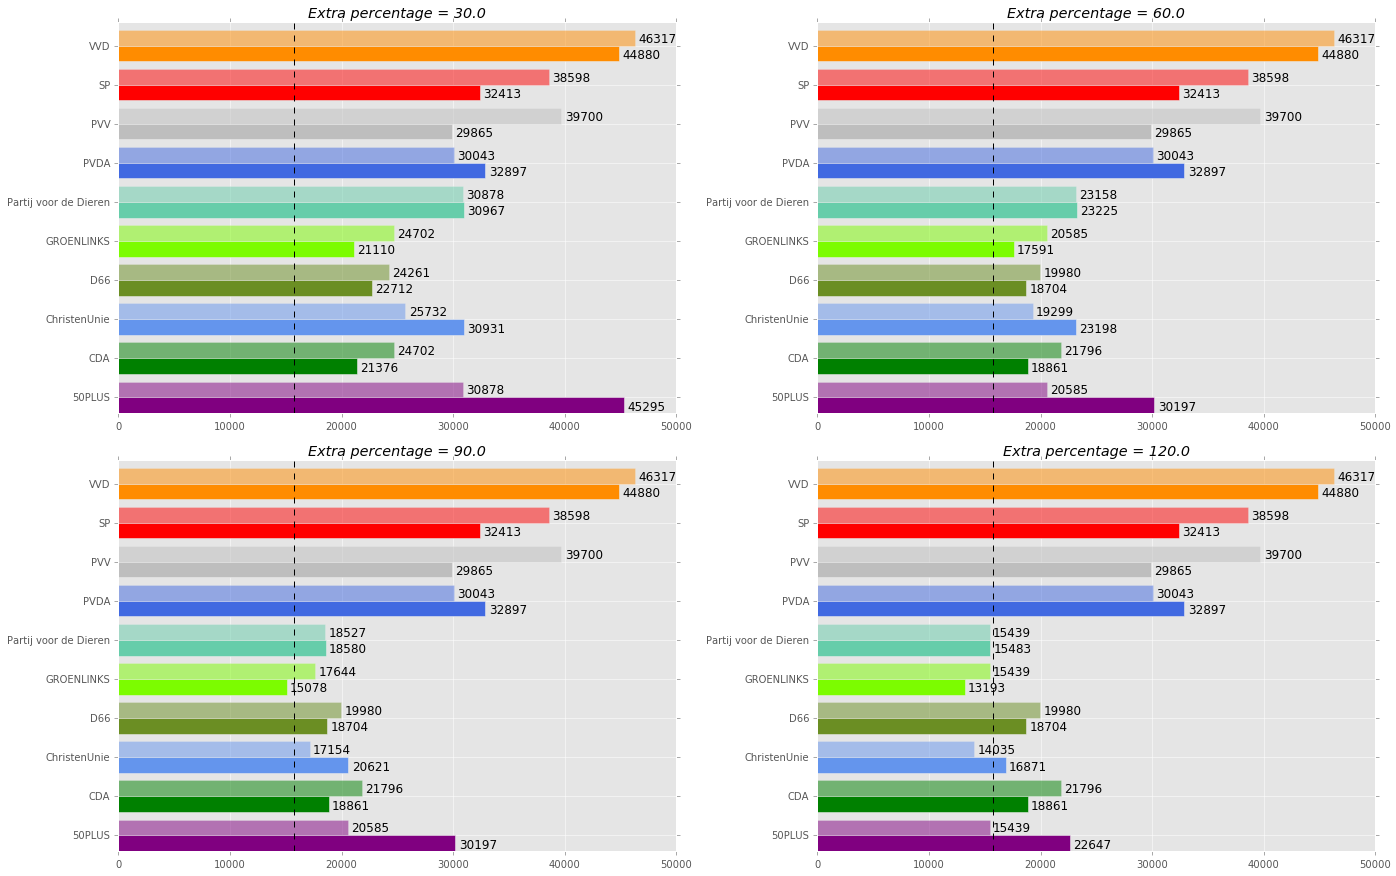
\includegraphics[width=\linewidth]	{stemmen_op_vrouwen_topNextrapercentage_samen.png}

			\caption{Grafieken in stappen van 30\%, met per partij de verdeling van de stemmen van vrouwelijk kiezers op de top \textit{N+extra percentage} vrouwelijke kandidaten van de partij a.d.h.v. de peiling \citep{IPSOS} in de licht gekleurd staven en a.d.h.v. de einduitslag \citep{Kiesraad_databank} in de donker gekleurde staven. De stippellijn is de daadwerkelijk voorkeursdrempel(15.708 stemmen).}

\label{fig:stemmenS4V}
\end{figure}


\paragraph{Aantal vrouwen na strategie 4.}
Na het uitvoeren van strategie 4 en het opstellen van de Tweede Kamer zoals eerder in dit hoofdstuk beschreven, zou strategie 4 bij geen enkel \textit{extra percentage} bovenop de originele \textit{N} uit strategie 1 een hoger aantal vrouwen op in de Tweede Kamer hebben opgeleverd. In de grafiek in Figuur \ref{fig:bcS4V} op de volgende pagina is te zien hoeveel vrouwen er in de Tweede Kamer een zetel bedeeld zouden hebben gekregen wanneer er een bepaald \textit{extra percentage} zou zijn toegevoegd aan de originele \textit{N} uit strategie 1. Zoals op de volgende pagina in Figuur \ref{fig:bcS4V} te zien, zouden er na uitvoering van strategie 4 en het toenemen van het \textit{extra percentage} op geen enkel punt meer vrouwen in de Tweede Kamer gekomen zijn dan de 121 uit strategie 1 (0\% staat in de grafiek gelijk aan strategie 1.) 


\begin{figure}[h]

	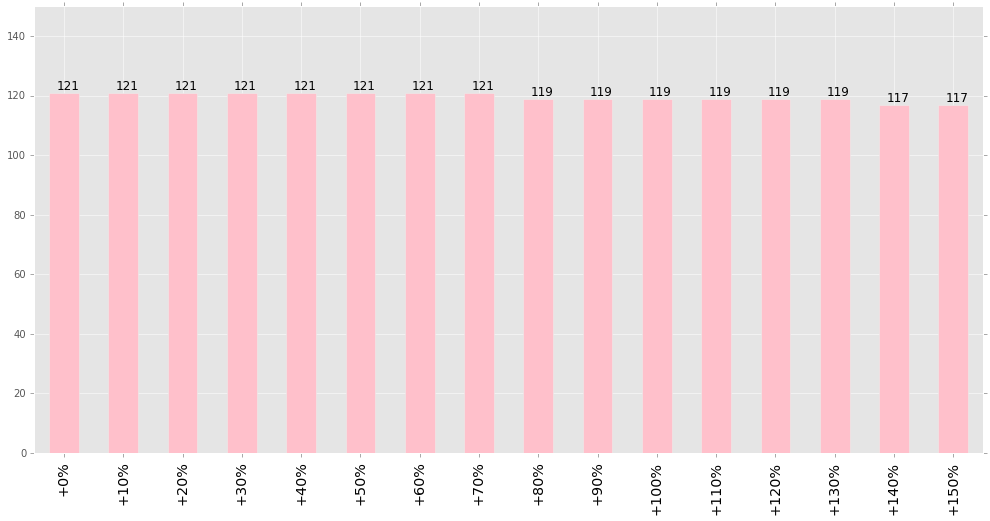
\includegraphics[width=\linewidth]	{topNextrapercentage_aantal_vrouwen_overzicht.png}

			\caption{Grafiek met per het aantal vrouwen in de Tweede Kamer na uitvoering(en) van strategie 4 in stappen van 10\% aan \textit{extra percentage} (van \textit{N}) bovenop de \textit{N} uit strategie 1.}

\label{fig:bcS4V}
\end{figure}

\paragraph{Niet meer dan 121 vrouwen in de Tweede Kamer.}
De reden dat er niet meer dan 121 vrouwen in de Tweede Kamer zouden hebben plaatsgenomen na uitvoering van strategie 4 ligt ten grondslag aan een aantal factoren. Wilden er meer vrouwen in de Tweede Kamer hebben plaatsgenomen dan na uitvoering van strategie 1 dan is het noodzakelijk dat de partijen ook meer zetels bedeeld kregen bij de einduitslag dan dat volgens te peiling was te verwachten. 

Zo kreeg het CDA bij de einduitslag dertien zetels bedeeld terwijl de peilingen aangaf dat het CDA twaalf zetels kon gaan verwachten. Vanwege het feit dat zowel de lijsttrekker, in de persoon van Sybrand van Haersma Buma, alsmede Pieter Omtzigt meer stemmen ontvingen dan de vrouwelijke kandidaten, blijven er nog elf zetels over die aan vrouwelijke kandidaten bedeeld hadden kunnen worden. Bij strategie 1 zouden de zetels al bedeeld zijn geweest aan deze elf vrouwelijke kandidaten.
D66 kreeg bij de einduitslag twaalf zetels bedeeld terwijl de peiling aangaf dat D66 elf zetels kon gaan verwachten. Vanwege het feit dat de lijsttrekker, in de persoon van Alexander Pechtold, meer stemmen ontving dan de vrouwelijke kandidaten, blijven er nog elf zetels over die aan vrouwelijke kandidaten bedeeld hadden kunnen worden. Bij strategie 1 zouden er al elf zetels aan vrouwelijke kandidaten bedeeld zijn geweest. De PVDA kreeg bij de einduitslag 38 zetels bedeeld terwijl de peiling aangaf dat de PVDA 36 zetels kon gaan verwachten. Vanwege het feit dat zowel de lijsttrekker, in de persoon van Diederik Samsom, als de nummer drie, Ronald Plasterk, meer stemmen ontvingen dan de vrouwelijke kandidaten, blijven er nog 36 zetels over die aan de vrouwelijke kandidaten bedeeld hadden kunnen worden. Bij strategie 1 zouden er al 36 zetels aan vrouwelijke kandidaten bedeeld zijn geweest. Ook de VVD kreeg bij de einduitslag meer zetels bedeeld dan dat zij volgens de peiling konden gaan verwachten (36 zetels bij de peiling en 41 zetels bij de einduitslag). Echter had de VVD maar 24 vrouwelijke kandidaten op de kandidatenlijst staan. Hierdoor kon de \textit{N+extra percentage} nooit meer dan 24 vrouwelijke kandidaten zijn. Alle vrouwelijke stemmen op de VVD zouden bij strategie 1 al over alle 24 vrouwelijke kandidaten verdeeld zijn geweest. 

De andere partijen ontvingen niet meer zetels bij de einduitslag dan dat zij volgens de peiling konden gaan verwachten. Zodoende had het aantal vrouwen die in de Tweede Kamer plaats zouden nemen nooit op meer dan 121 kunnen uitkomen.   






\newpage
\section{Factoren en Invloed}
\label{h5}



\subsection*{Deelvraag 2: Welke factoren kunnen per bevolkingsgroep van invloed zijn op het wel of niet behalen van het maximum aantal kandidaten dat in de Tweede Kamer gekozen kan worden?}
Voor het behalen van het maximum per bevolkingsgroep zijn er een aantal factoren die van invloed kunnen zijn. Deze factoren kunnen invloed uitoefenen op mate van een succes van een door een bevolkingsgroep gekozen strategie. Alvorens we per specifieke bevolkingsgroep de factoren en de invloed van deze factoren gaan beschrijven, zullen we eerst de algemene factoren beschrijven die van invloed (kunnen) zijn op elke bevolkingsgroep.

\subsubsection*{Algemene factoren.}
De algemene factoren zijn de factoren die van invloed kunnen zijn op elke bevolkingsgroep. In deze sectie worden deze algemene factoren kort beschreven alvorens in de volgende secties er per specifieke bevolkingsgroep dieper op de factoren wordt ingegaan. De algemene factoren zijn:\\

\newcolumntype{L}{@{}>{\bfseries}p{14em}<{}}% Item label
\newcolumntype{I}{X@{}}% Item contents
\noindent\begin{tabularx}{\textwidth}{LI}
Aantal kandidaten: &  Voor het kunnen toepassen van één van de in het vorige hoofdstuk toegepaste strategie\"{e}n, is het in eerste instantie essentieel dat er \"{u}berhaupt kandidaten van een bevolkingsgroep op de kandidatenlijsten staan. Daarnaast is het aantal kandidaten van de belang om bijvoorbeeld een volledig door één bevolkingsgroep bezette Tweede Kamer te vormen. In de volgende secties betreffende de factoren per bevolkingsgroep wordt hier dieper op ingegaan. \\
\\ 
Keuze strategie: &  Een keuze van een strategie kan van invloed zijn op het wel of niet behalen van het theoretisch maximum. Een strategie kan moeilijk te communiceren zijn binnen een bevolkingsgroep en gemakkelijk te manipuleren zijn door 'tegenstanders'.\\
\\ 
Committeren aan strategie:  & In het vorige hoofdstuk is telkens per bevolkingsgroep onderzocht wat het theoretisch maximum is wanneer 100\% van de kiesgerechtigden zich committeert aan een strategie. Echter is het de vraag wat er gebeurt als een bepaald percentage van een bevolkingsgroep zich committeert aan een strategie. Waar het theoretisch maximum uitgaat van 100\% deelname van de leden van een bevolkingsgroep is dit in de praktijk moeilijk haalbaar. Het is daarom interessant te onderzoeken wat het theoretisch maximum per bevolkingsgroep is wanneer de meeste succesvolle strategie uit het vorige hoofdstuk wordt uitgevoerd door een deel van de bevolkingsgroep.  \\
\\
\end{tabularx}  
 
 \newcolumntype{L}{@{}>{\bfseries}p{14em}<{}}% Item label
\newcolumntype{I}{X@{}}% Item contents
\noindent\begin{tabularx}{\textwidth}{LI}

Tegenstrategie: & Een bevolkingsgroep met tegengestelde eigenschappen (bijvoorbeeld de bevolkingsgroep mannen tegenover vrouwen) zou een tegenstrategie zouden kunnen toepassen om te verhinderen dat tegengestelden in hogere mate vertegenwoordigd worden in de Tweede Kamer. In Hoofdstuk \ref{h7} wordt er dieper ingegaan op wat er kan gebeuren wanneer meerdere bevolkingsgroepen een strategie uitvoeren.\\
\\
 \end{tabularx}  


\paragraph{Overzicht bevindingen.}
Voordat we per bevolkingsgroep dieper in gaan op de factoren en de invloed die deze factoren hebben, worden hieronder eerst de belangrijkste bevindingen op een rijtje gezet. De bevindingen zijn:

\begin{itemize}
\item
Alle bevolkingsgroepen hebben een voldoende aantal kandidaten op de kandidatenlijsten staan. Enkel de SGP heeft zowel geen vrouwelijke alsmede allochtone kandidaten op de kandidatenlijst staan. De Partij voor de Dieren heeft geen allochtone kandidaten op de kandidatenlijst staan.
\item
Strategie 1 en strategie 2 zouden bij een deelname van slechts 40\% van de leden van de bevolkingsgroepen een hoog rendement hebben opgeleverd.
\item
De bevolkingsgroep vrouwen lijkt de bevolkingsgroep te zijn waar de meeste animo onder de bevolkingsleden bestaat als het gaat om zich te committeren aan een strategie om zodoende adequater vertegenwoordigd te worden in de Tweede Kamer. 

\item
Wat betreft het hanteren van een tegenstrategie is het moeilijk te concluderen welke bevolkingsgroepen het meest waarschijnlijk zouden kunnen worden tegengewerkt wanneer zij een strategie uit willen voeren. Echter lijkt het bij de bevolkingsgroep allochtonen en, in minder mate,  de bevolkingsgroep vrouwen het meest waarschijnlijk dat er vanuit de samenleving een tegenbeweging kan ontstaan.


\end{itemize}



\subsection{Factoren bevolkingsgroep vrouwen.}
\label{percV}

\paragraph{Aantal Vrouwelijke Kandidaten.}
Zoals in het vorige hoofdstuk al is beschreven was het bij de Tweede Kamerverkiezingen van 2012 onmogelijk om een Tweede Kamer te vorm die volledig werd bezet door vrouwelijke kamerleden. De SGP had helemaal geen vrouwelijke kandidaten op de kandidatenlijst en de PVV en de VVD hadden een hoger aantal zetels ontvangen dan het aantal vrouwelijke kandidaten dat deze partijen op de kandidatenlijsten hadden. Echter waren er bij de partijen die zetels hebben ontvangen toch het totaal van 179 vrouwelijke kandidaten waarop gestemd kon worden(zie Figuur \ref{fig:aaKandidaten} in Hoofdstuk  \ref{sec:math}). 

\paragraph{Keuze Strategie.}
Wat betreft het kiezen van een strategie is strategie 1 de strategie die bij de bevolkingsgroep vrouwen het meeste succes zou hebben opgeleverd. Zoals we weten, zou strategie 1 het theoretisch maximum van 121 vrouwen in de Tweede Kamer. Echter levert strategie 2 ook een hoog rendement met 116 vrouwen in de Tweede Kamer. In de volgende paragraaf wordt er dieper ingegaan op wat er had gebeurd wanneer een deel van de bevolkingsgroep zich zou hebben gecommitteerd aan strategie 1 of strategie 2.

\paragraph{Committeren aan een strategie.}
Sinds de dagen van Aletta Jacobs en het ontstaan van de \textit{Eerste Feministische Golf} \citep{braun1992prijs}, de \textit{Dolle Mina's} en de \textit{Man Vrouw Maatschappij} in de jaren '60 en het ontstaan van de \textit{Tweede Feministische Golf} \citep{van2005vrouw} zijn er in de loop der jaren tal van personen en organisaties in Nederland bij gekomen die de belangen van vrouwen behartigen. Een kleine greep uit Nederlandse vrouwenbelangen organisaties levert op: de Nederlandse Bond voor Vrouwenkiesrecht, Nederlandse Unie voor Vrouwenbelangen, de Nederlandse Vrouwenraad, FNV Vrouw, Vereniging Vrouw en Recht etc. Daarnaast is minister Bussemaker van Onderwijs, Cultuur en Wetenschap \citeyearpar{navigerennaardetop} campagne begonnen die ervoor moet zorgen dat er meer vrouwen in topfuncties komen in Nederland. Volgens \cite{van2012tweede} krijgen met name de hoogstgeplaatste vrouwelijke kandidaten op de kandidatenlijsten een voorkeurstemmen van de vrouwelijke kiezer vanwege het feit dat de kandidaat van hetzelfde geslacht is. Tevens is het zo dat de hoogstgeplaatste vrouwelijke kandidaten op de kandidatenlijsten (de vrouwelijke lijsttrekkers buiten beschouwing gelaten) een hoog aantal voorkeurstemmen ontvangen. In Tabel \ref{table:HoogstV} is te zien dat zeven hoogstgeplaatste vrouwelijke kandidaten bij de offici\"{e}le verkiezingsuitslag genoeg stemmen hebben ontvangen om boven de voorkeursdrempel uit te komen. Het gemiddelde bij de hoogstgeplaatste vrouwelijke kandidaten ligt maar liefst op het aantal van 66.419 stemmen. Er kan daarmee worden aangenomen dat er een zekere animo bestaat bij Nederlandse vrouwen om zich te committeren aan een strategie die ervoor moet zorgen dat vrouwen in hogere mate vertegenwoordigd worden in de Tweede Kamer. 


\begin{table}[H]
\centering
	\begin{footnotesize}
		\begin{tabular}{llrr}
\toprule
{} &                 Partij &  Plaats op Lijst &  Aantal Stemmen  \\
Kandidaat                                &                        &                  &    Kandidaat                       \\
\midrule
M.H.H. (Martine) Baay-Timmerman          &                 50PLUS &                3 &                      7123 \\
M.C.G. (Mona) Keijzer                    &                    CDA &                2 &                    127446 \\
C.J. (Carola) Schouten                   &           ChristenUnie &                3 &                     16507 \\
S. (Stientje) van Veldhoven-van der Meer &                    D66 &                2 &                     71170 \\
L. (Liesbeth) van Tongeren               &             GROENLINKS &                3 &                     10205 \\
E. (Esther) Ouwehand                     &  Partij v d Dieren &                2 &                     11573 \\
J. (Jetta) Klijnsma                      &                   PVDA &                2 &                    192190 \\
M. (Fleur) Agema                         &                    PVV &                2 &                     34943 \\
R.M. (Renske) Leijten                    &                     SP &                2 &                     69146 \\
E.I. (Edith) Schippers                   &                    VVD &                2 &                    123889 \\
\bottomrule
\end{tabular}

	\end{footnotesize}
			\caption{Het aantal stemmen dat de hoogstgeplaatste vrouwelijke kandidaten hebben ontvangen volgens de offci\"{e}le einduitslag. De SGP had geen vrouwelijke kandidaten.}
\label{table:HoogstV} 
\end{table} 

\indent Een deelname van 100\% van de vrouwelijke kiezers aan strategie 1 zou een Tweede Kamer op hebben kunnen leveren waarin 121 vrouwen plaats zouden hebben genomen en bij strategie 2 zouden er 116 vrouwen plaats hebben genomen (zie Sectie \ref{vrouwen}. Echter is het de vraag wat er had gebeurd wanneer niet de volle 100\% van de vrouwelijke kiezers zich had gecommitteerd maar een 'slechts' een deel van de vrouwelijke kiezers. In Figuur \ref{fig:PerV} is te zien hoeveel zetels er aan vrouwelijk kandidaten bedeeld zouden zijn wanneer een bepaald percentage van de vrouwelijke kiezers zich had gecommitteerd aan strategie 1 (blauwe staven) of strategie 2 (groene staven). Hierbij moet genoteerd worden dat het aantal stemmen van vrouwelijke kiezers op een partij een percentage is van het totaal door vrouwelijke kiezers uitgebrachte stemmen (100\% deelname van vrouwelijke kiezers). Tevens nemen we aan dat het percentage van de vrouwelijke kiezers die zich committeren aan een strategie voor elke partij hetzelfde is. Oftewel wanneer bijvoorbeeld 25\% van de vrouwelijke kiezers zich committeren aan de strategie dan is geldt de 25\% voor elke partij. Ter illustratie het nemen we de VVD als voorbeeld.

De VVD had volgens de einduitslag van de Tweede Kamerverkiezingen van 2012 een totaal van 1.077.127 vrouwelijke stemmen ontvangen (zie Figuur \ref{table:tab2V} in Sectie \ref{vrouwen}). Wanneer 25\% van de vrouwelijke kiezers zich committeren aan strategie 1 of strategie 2 leveren deze strategie\"{e}n bij de VVD het aantal van ($25\%*1.077.127$ = ) 269.281 vrouwelijke stemmen stemmen op. De overige stemmen van vrouwelijke kiezers op de VVD laten we buiten beschouwing vanwege het feit dat we niet kunnen voorspellen naar welke partij of kandidaat deze stemmen gaan. Derhalve kunnen we alleen het aantal stemmen in ogenschouw nemen wat zekerheid biedt voor het berekenen van het aantal stemmen dat vrouwelijke kandidaten van vrouwelijk kiezers zouden gaan ontvangen om zodoende vrouwelijke kandidaten boven de kiesdrempel te helpen.  

In Figuur \ref{fig:PerV} is te zien dat wanneer slechts 70\% van de vrouwelijke kiezers zich had gecommitteerd aan strategie 1, het maximum aantal nog zou zijn behaald. Bij 60\% van de vrouwelijke kiezers viel er bij strategie 1 één enkele vrouwelijke kandidaat af en bij slechts 50\% van de vrouwelijke kiezers zouden er nog altijd 36 vrouwen meer in de Tweede Kamer plaats hebben genomen dan daadwerkelijk bij de offci\"{e}le einduitslag het geval was (58 vrouwen in de Tweede Kamer na de offci\"{e}le einduitslag). 

Voor strategie 2 is te zien dat het maximum aantal dat mogelijk zou zijn geweest met uitvoering van strategie 2, behaald werd wanneer 85\% van de vrouwelijke kiezers zich had gecommitteerd aan strategie 2. Bij slechts 50\% van de vrouwelijke kiezers zouden er nog altijd 33 vrouwen meer in de Tweede Kamer plaats hebben genomen dan daadwerkelijk bij de offci\"{e}le einduitslag het geval was.

\begin{figure}[H]


	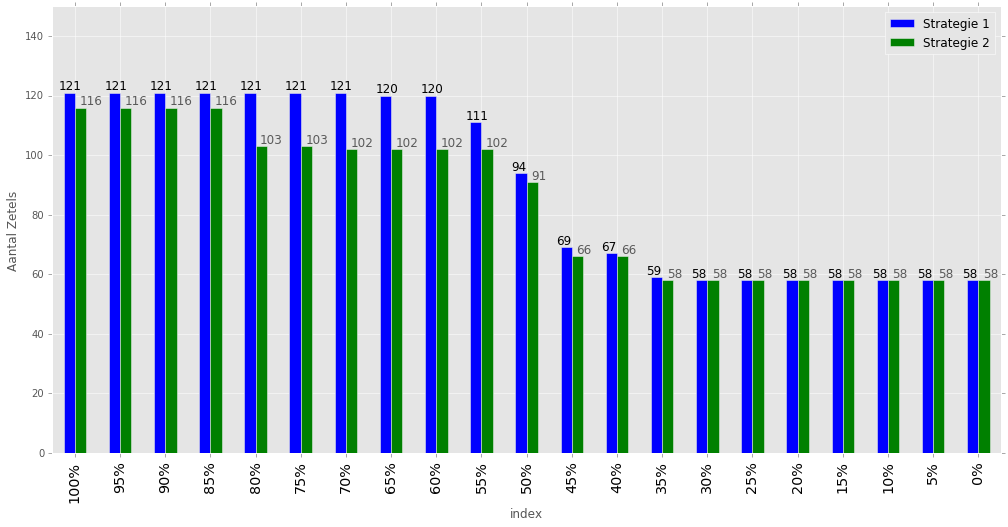
\includegraphics[width=\linewidth]{percentages_van_vrouwenS1S2.png}

			\caption{Grafiek met overzicht van het maximum aantal zetels wat behaald kon worden wanneer een bepaald percentage van de vrouwelijke kiezers zich committeerde aan strategie 1.}

\label{fig:PerV}
\end{figure}






\paragraph{Tegenstrategie.}
Uit een onderzoek van \cite{lawless2012men} blijkt dat mannen in de Verenigde Staten het eigen geslacht geschikter achten voor het bekleden van een politieke ambt dan het vrouwelijk geslacht. Een vergelijkbaar onderzoek betreffende mannen en vrouwen in Nederland ontbreekt echter. Hoewel een onderzoek van \cite{mcelroy2009candidate} aangeeft dat kiezers in landen waar verkiezingen met een voorkeursstemregel niet discrimineren op basis van geslacht, is het mogelijk dat mannen het eigen geslacht prefereren als het gaat om het kiezen van vertegenwoordigers in de Tweede Kamer. Zodoende is het niet ondenkbaar dat mannen een tegenstrategie zullen toepassen om te voorkomen dat de vrouwen in hogere mate vertegenwoordigd woorden dan eerder het geval is geweest. 

\subsection{Factoren bevolkingsgroep allochtonen.}

\paragraph{Aantal allochtone Kandidaten.} 
Zoals in het vorige hoofdstuk al is beschreven was het bij de Tweede Kamerverkiezingen van 2012 onmogelijk om een Tweede Kamer te vorm die volledig werd bezet door allochtone politici. De SGP en de Partij voor de Dieren hadden geen enkele allochtoon op de kandidatenlijsten staan en, op 50PLUS en GROENLINKS na, ontvingen alle partijen bij de einduitslag meer zetels dan het aantal allochtonen dat zij op de kandidatenlijsten hadden staan. In totaal stonden er, bij de partijen die zetels hebben ontvangen, vijftig allochtone kandidaten op de kandidatenlijsten (zie Figuur \ref{fig:aaKandidaten} in Hoofdstuk \ref{sec:meth}). 

\paragraph{Keuze Strategie.}
Wat betreft het kiezen van een strategie maakt het voor de bevolkingsgroep allochtonen niet uit of strategie 1 of strategie 2 wordt uitgevoerd wanneer de volle 100\% van de allochtone kiezers zich committeren aan de strategie. Ook bij het uitvoeren van strategie 2 waarbij slechts een deel van de allochtone kiezers zich committeert aan de strategie is het resultaat hetzelfde. Het maakt geen verschil of er voor strategie 1 of strategie 2 wordt gekozen. In de volgende paragraaf wordt er dieper ingegaan op wat er had gebeurd wanneer een deel van de bevolkingsgroep zich zou hebben gecommitteerd aan strategie 1 of strategie 2.



\paragraph{Committeren aan een strategie.}
Uit onderzoek van \citep{fennema2001civic} blijkt dat met name allochtonen van Turkse en Marokkaanse afkomst geneigd zijn op een kandidaat te stemmen met dezelfde afkomst. Echter lijken allochtone kiezers van Turkse afkomst in hogere mate te mobiliseren als het gaat om het uitbrengen van een stem bij de Tweede Kamerverkiezingen dan allochtonen van Marokkaanse afkomst. Onderzoek betreffende allochtonen met een andere afkomst dan een Turkse of Marokkaanse ontbreekt echter. Als het gaat om verbondenheid tussen etnische minderheden voelen personen behorende tot verschillende etnische minderheden zich in sterkere mate met elkaar verbonden wanneer zij zich benadeeld of minder geaccepteerd voelen \citep{schmitt2002meaning}. Volgens \cite{buijs2006strijders} voelen veel allochtonen in Nederland, van met name Turkse en Marokkaanse achtergrond, zich niet geaccepteerd. Volgens \cite{van2012tweede} geldt ook voor allochtonen dat zij in de meeste voorkeurstemmen uitbrengen op de hoogstgeplaatste allochtone kandidaat op de kandidatenlijst. In Tabel \ref{table:HoogstA} is te zien dat van de hoogstgeplaatste allochtone kandidaten op de kandidatenlijsten er slechts één allochtone kandidaat, in de persoon van Tanja Jadnanansing, boven de voorkeursdrempel uit is gekomen. Of dit ligt aan het feit dat zij stemmen van allochtone kiezers heeft gekregen, stemmen van vrouwelijke kiezers heeft gekregen of een combinatie ven beiden is niet duidelijk. Het gemiddelde bij de hoogstgeplaatste allochtone kandidaten lag op het aantal van 7.420 stemmen. Afgaande op het het aantal stemmen op de hoogstgeplaatste allochtone kandidaat lijkt de stelling van \cite{van2012tweede} niet helemaal op te gaan. Echter kan uit de eerdere stelling in deze paragraaf wel worden afgeleid dat er animo kan bestaan onder allochtonen om zich te committeren aan een strategie die ervoor moet zorgen dat allochtonen in hogere mate vertegenwoordigd worden in de Tweede Kamer. \\

\begin{table}[H]
\centering
	\begin{footnotesize}
		\begin{tabular}{lllrr}
\toprule
{} & Geslacht &        Partij &  Plaats op Lijst &  Aantal Stemmen Kandidaat \\
Kandidaat                 &          &               &                  &                           \\
\midrule
K.L.R. (Roy) Ho Ten Soeng &        M &        50PLUS &                6 &                      2654 \\
M. (Mustafa) Amhaouch     &        M &           CDA &               16 &                      1919 \\
I.S. (Ixora) Balootje     &        V &  ChristenUnie &                9 &                      2111 \\
V.A. (Vera) Bergkamp      &        V &           D66 &                5 &                     15387 \\
J.F. (Jesse) Klaver       &        M &    GROENLINKS &                4 &                      3351 \\
T.M. (Tanja) Jadnanansing &        V &          PVDA &                4 &                     28704 \\
J.D. (Jenny) Zerfowski    &        V &           PVV &               37 &                       210 \\
S. (Sadet) Karabulut      &        V &            SP &                6 &                     10572 \\
M. (Malik) Azmani         &        M &           VVD &               20 &                      1874 \\
\bottomrule
\end{tabular}

	\end{footnotesize}
			\caption{Het aantal stemmen dat de hoogstgeplaatste allochtone kandidaten hebben ontvangen volgens de offci\"{e}le einduitslag.}
\label{table:HoogstA} 
\end{table}





\indent Een deelname van 100\% van de allochtone kiezers aan strategie 1 of strategie 2 zou een Tweede Kamer hebben opgeleverd waarin 34 allochtonen plaatsen zouden nemen (zie Sectie \ref{allochtonen}). Ook bij de bevolkingsgroep allochtonen gaan we onderzoek wat er gebeurt wanneer een deel van de bevolkingsgroep zich committeert aan strategie 1 of strategie 2. Op dezelfde wijze als bij de bevolkingsgroep vrouwen is gedaan, gaan we berekenen hoeveel zetels er aan allochtone kandidaten bedeeld zouden zijn wanneer bepaalde percentages van de bevolkingsgroep allochtonen zich had gecommitteerd aan strategie 1 of strategie 2 (zie Sectie \ref{percV} voor uitleg van het bereken van het aantal stemmen). In Figuur\ref{fig:PerA} is te zien hoeveel zetels er aan allochtone kandidaten zouden zijn bedeeld wanneer een bepaald percentage van de allochtone kiezers zich had gecommitteerd aan strategie 1 (blauwe staven) of strategie 2 (groene staven).  

\begin{figure}[H]


	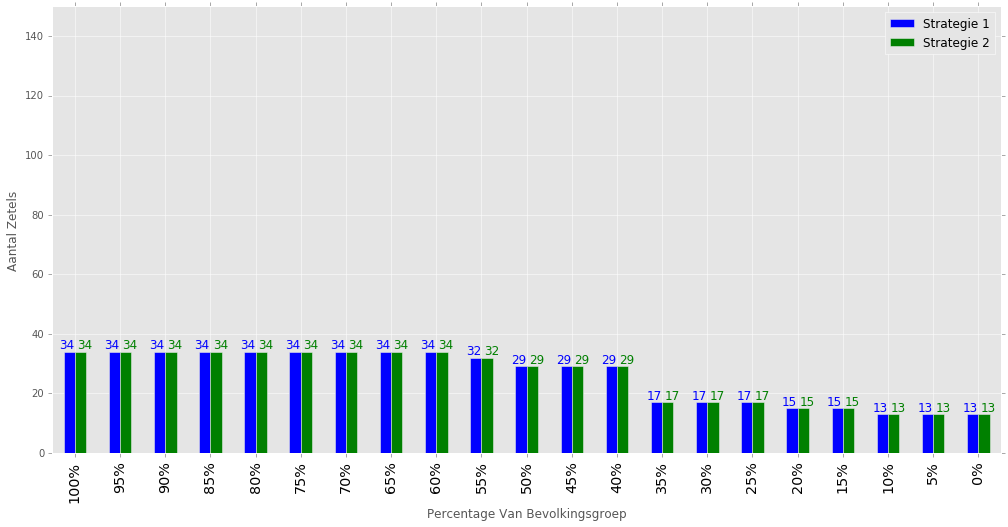
\includegraphics[width=\linewidth]{percentages_van_allochtonenS1S2.png}

			\caption{Grafiek met overzicht van het maximum aantal zetels wat behaald kon worden wanneer een bepaald percentage van de allochtone kiezers zich committeerde aan strategie 1 (blauwe staven) of strategie 2 (groene staven).}

\label{fig:PerA}
\end{figure}

In Figuur \ref{fig:PerA} is te zien dat wanneer slechts 60\% van de allochtone kiezers zich had gecommitteerd aan strategie 1 of strategie 2, het maximum aantal nog altijd werd behaald. Bij 40\% van de vrouwelijke kiezers zoude er vijf allochtone kandidaten afvallen en bij slechts 25\% van de allochtone kiezers zijn er bij beiden strategie\"{e}n nog altijd vier allochtonen meer in de Tweede Kamer dan daadwerkelijk bij de offci\"{e}le einduitslag het geval was (dertien allochtonen in de Tweede Kamer na de offci\"{e}le einduitslag). Beiden strategie\"{e}n hadden voor elk percentage aan deelnemers hetzelfde rendement opgeleverd.




\paragraph{Tegenstrategie.}
Volgens een artikel van \cite{de2000political} blijkt het zo te zijn dat rechtse partijen in zowel Nederland als Vlaanderen (bijvoorbeeld het Vlaams Blok) kiezers voor zich weten te winnen op basis van een negatief beeld dat deze kiezers hebben als het gaat om allochtonen- en migrantenkwesties. Daarnaast speelt ook chauvinisme een rol als het gaat om het stemmen op autochtone kandidaten en populistische partijen \citep{van2010swaying}. Hierdoor is het niet ondenkbaar dat een groep autochtone kiezers een tegenstrategie zal uitvoeren om juist meer autochtone kandidaten in de Tweede Kamer te krijgen.

\subsection{Factoren bevolkingsgroep ouderen.}
\label{percO}

\paragraph{Aantal oudere Kandidaten.} 
Zoals in het vorige hoofdstuk al is beschreven was het bij de Tweede Kamerverkiezingen van 2012 onmogelijk om een Tweede Kamer te vorm die volledig werd bezet door oudere politici. Het CDA, de PVDA, de VVD, de SP, D66 en de SGP ontvingen meer zetels dan dat zij oudere kandidaten op de kandidatenlijst hadden staan. In totaal stonden er, bij de partijen die zetels hebben ontvangen, 135 oudere kandidaten op de kandidatenlijsten (zie Figuur \ref{fig:jaKandidaten} in Hoofdstuk \ref{sec:math})

\paragraph{Keuze Strategie.}
Wat betreft het kiezen van een strategie is strategie 1 de strategie die het meeste succes opleverde bij de bevolkingsgroep ouderen. Zoals we weten, leverde strategie 1 het theoretisch maximum van 89 ouderen in de Tweede Kamer op. Echter levert strategie 2 ook een hoog rendement met 84 ouderen in de Tweede Kamer. In de volgende paragraaf wordt er dieper ingegaan op wat er had gebeurd wanneer een deel van de bevolkingsgroep zich zou hebben gecommitteerd aan strategie 1 of strategie 2.

\paragraph{Committeren aan een strategie.}
In de literatuur bestaat er geen onderzoek betreffende voorkeurstemmen op oudere kandidaten. Echter kan aan de hand van de verkiezingseinduitslag worden opgemaakt dat er weinig sentimenten leven onder ouderen om beter vertegenwoordigd te worden door oudere politici in de Tweede Kamer. Een partij die specifiek opkomt voor belangen van ouderen is 50PLUS. Het feit dat 50PLUS slechts 4\% van de stemmen van ouderen heeft gekregen (zie Figuur \ref{fig:zetelsO} in Sectie \ref{ouderen}) suggereert dat ouderen ook andere aandachtspunten dan het zijn van een oudere belangrijk vinden als het gaat om het uitbrengen van een stem. Tevens is het zo dat de hoogstgeplaatste ouderen op de kandidatenlijsten (de lijsttrekkers buiten beschouwing gelaten) over het algemeen weinig voorkeurstemmen hebben ontvangen. In Tabel \ref{table:HoogstO} is te zien dat enkel Fred Teeven van de VVD en Jetta Klijnsma van de PVDA genoeg stemmen hebben ontvangen om boven de voorkeursdrempel uit te komen. Echter genieten deze politici een grote mate van bekendheid in Nederland en stonden zij hoog op de kandidatenlijsten. Hetgeen een goeie indicatie is voor het krijgen van voorkeurstemmen \citep{van2012tweede}. Het gemiddelde bij de hoogstgeplaatste oudere kandidaten lag op het aantal van 22.937 stemmen. Echter wordt het gemiddelde door het grote aantal voorkeurstemmen dat Jette Klijnsma ontving flink omhoog gekrikt. Het feit dat Jetta Klijnsma zo veel stemmen heeft ontvangen ligt waarschijnlijk ten grondslag aan het feit dat, zoals eerder al is aangegeven, vrouwelijke kiezers geneigd zijn om op de hoogstgeplaatste vrouwelijke kandidaat te stemmen. Het lijkt daarmee onwaarschijnlijk dat Jetta Klijnsma zo veel stemmen heeft ontvangen vanwege het feit dat zij een oudere is. Dit alles doet vermoeden dat het onwaarschijnlijk lijkt dat ouderen zich zullen committeren aan een strategie. Desalniettemin, of misschien wel des te meer, is het interessant om te onderzoek wat het theoretisch maximum is wanneer een deel van de oudere kandidaten zich committeert aan een strategie. \\

\begin{table}[H]
\centering
	\begin{footnotesize}
		\begin{tabular}{lllrr}
\toprule
{} & Geslacht &                 Partij &  Plaats   &  Aantal Stemmen  \\
 & & & op Lijst & Kandidaat\\
Kandidaat                                &          &                        &                  &                           \\
\midrule
N.P.M. (Norbert) Klein       &        M &                 50PLUS &                2 &                      3511 \\
P. (Peter) Oskam             &        M &                    CDA &               10 &                       702 \\
C.P. (Onno) van Schayck      &        M &           ChristenUnie &               17 &                       307 \\
P.H. (Paul) van Meenen       &        M &                    D66 &                7 &                      1802 \\
A. (Bram) van Ojik           &        M &             GROENLINKS &                2 &                      4639 \\
B.E.J.M. (Birgit) Verstappen &        V &  Partij voor de Dieren &                7 &                       844 \\
J. (Jetta) Klijnsma          &        V &                   PVDA &                2 &                    192190 \\
L. (Louis) Bontes            &        M &                    PVV &                5 &                       958 \\
R. (Roelof) Bisschop         &        M &                    SGP &                3 &                      2234 \\
H. (Harry) van Bommel        &        M &                     SP &                4 &                     10021 \\
F. (Fred) Teeven             &        M &                    VVD &                5 &                     35103 \\
\bottomrule
\end{tabular}

	\end{footnotesize}
			\caption{Het aantal stemmen dat de hoogstgeplaatste oudere kandidaten hebben ontvangen volgens de offci\"{e}le einduitslag.}
\label{table:HoogstO} 
\end{table}

\indent Een deelname van 100\% van de oudere kiezers aan strategie 1 zou in een Tweede Kamer hebben opgeleverd waarin 89 ouderen plaats zouden nemen en bij strategie 2 zouden er 84 ouderen hebben plaatsgenomen (zie Sectie \ref{ouderen}. Op dezelfde wijze als bij de bevolkingsgroep vrouwen is gedaan, gaan we berekenen hoeveel zetels er aan oudere kandidaten worden bedeeld wanneer bepaalde percentages van de bevolkingsgroep ouderen zich committeert aan de strategie (zie Sectie \ref{percV} voor uitleg van het bereken van het aantal stemmen). In Figuur \ref{fig:PerO} is te zien hoeveel zetels er aan oudere kandidaten zouden zijn bedeeld wanneer een bepaald percentage van de oudere kiezers zich had gecommitteerd aan strategie 1 of strategie 2.  



\begin{figure}[H]
	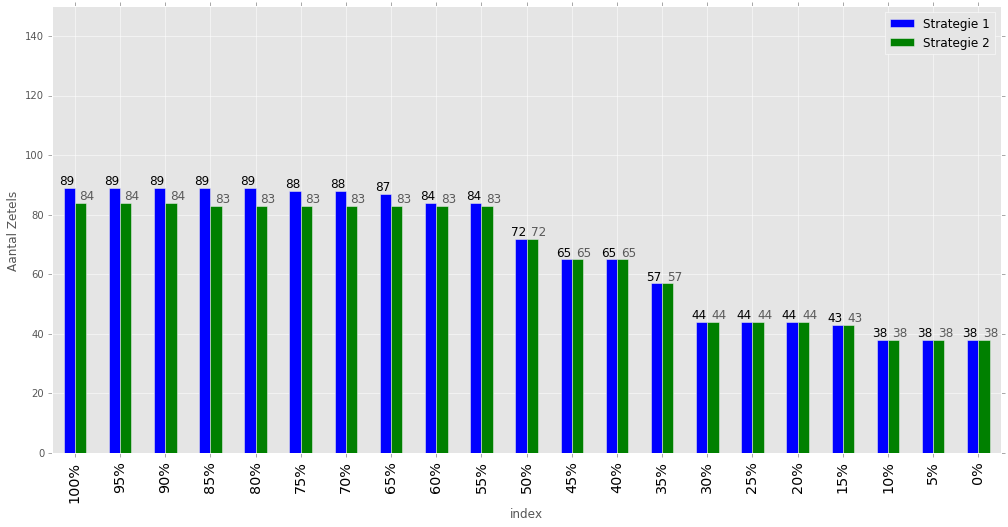
\includegraphics[width=\linewidth]{percentages_van_ouderenS1S2.png}

			\caption{Grafiek met overzicht van het maximum aantal zetels wat behaald kon worden wanneer een bepaald percentage van de oudere kiezers zich committeerde aan strategie 1.}

\label{fig:PerO}
\end{figure}

In Figuur \ref{fig:PerO} is te zien dat wanneer 80\% van de oudere kiezers zich had gecommitteerd aan strategie 1, het maximum aantal nog altijd zou zijn behaald. Bij 55\% van de oudere kiezers vielen er vijf oudere kandidaten af en bij slechts 35\% van de oudere kiezers zijn er nog altijd negentien ouderen meer in de Tweede Kamer dan daadwerkelijk bij de offci\"{e}le einduitslag het geval was (38 ouderen in de Tweede Kamer na de offci\"{e}le einduitslag). 

Voor strategie 2 is te zien dat het maximum aantal dat mogelijk zou zijn geweest met uitvoering van strategie 2, behaald werd wanneer 90\% van de oudere kiezers zich had gecommitteerd aan strategie 2. Bij slechts 50\% van de oudere kiezers zouden er nog altijd 35 ouderen meer in de Tweede Kamer plaats hebben genomen dan daadwerkelijk bij de offci\"{e}le einduitslag het geval was.



\paragraph{Tegenstrategie.}
Volgens \cite{aalberts2006aantrekkelijke} vinden met name jongeren dat politici te oud zijn. Echter is het de vraag in hoeverre dit invloed zou kunnen hebben op hun partij- of kandidatenkeuze. Hoewel misschien onwaarschijnlijk is het niet ondenkbaar dat een groep opstaat en zich samen aan een strategie committeert om zodoende te zorgen dat er juist minder oudere kandidaten in de Tweede Kamer plaatsnemen. 

\subsection{Factoren bevolkingsgroep provincialen.}
\label{percP}

\paragraph{Aantal provinciale Kandidaten.} 
Bij \hyperref[S1A]{strategie 1} voor de bevolkingsgroep provincialen werd beschreven dat gezien de peiling en het bepalen van de top \textit{N} provinciale kandidaten er niet meer dan 147 provinciale kandidaten gekozen konden worden. Dit vanwege het feit dat de SP minder provinciale kandidaten op de kandidatenlijst had staan dan verwacht werd dat zij zetels zouden gaan ontvangen (zie Strategie \ref{sssec:S1P} in Sectie \ref{provincialen}). Echter de peiling correspondeerde niet 100\% met de uiteindelijke einduitslag. Op de PVDA na hadden alle partijen en hoger aantal provinciale kandidaten dan het aantal zetels dat zij a.d.h.v. de einduitslag bedeeld kregen. De PVDA had echter één zetels minder ontvangen dan het aantal provinciale kandidaten dat zij op de kandidatenlijsten hadden staan. Er hadden een totaal van 149 provincialen in de Tweede Kamer gekozen kunnen worden. Hierdoor had een Tweede Kamer bestaande uit enkel provincialen net niet mogelijk geweest. In totaal stonden er, bij de partijen die zetels hebben ontvangen, 235 oudere kandidaten op de kandidatenlijsten (zie Figuur \ref{fig:rpKandidaten} in Hoofdstuk \ref{sec:meth}).

\paragraph{Keuze Strategie.}
Wat betreft het kiezen van een strategie is strategie 1 niet de strategie die het meeste succes opleverde bij de bevolkingsgroep provincialen. Zoals aangetoond bij de uitvoering van \hyperref[S4P]{strategie 4} in Bijlage \ref{provincialen}, leverde strategie 4 het theoretisch maximum van 142 provincialen in de Tweede Kamer. Hierbij diende de \textit{N} te worden uitgebreid met een \textit{extra percentage=20}. Strategie 1 zou ook een hoog rendement hebben opgeleverd met 138 provincialen in de Tweede Kamer en ook strategie 2 zou met 131 provincialen in de Tweede Kamer een hoog rendement hebben opgeleverd. In de volgende paragraaf wordt er dieper ingegaan op wat er had gebeurd wanneer een deel van de bevolkingsgroep zich zou hebben gecommitteerd aan strategie 1, strategie 2 of strategie 4.

\paragraph{Committeren aan een strategie.}
In de literatuur bestaat er geen onderzoek betreffende voorkeurstemmen op provinciale kandidaten. Echter kan aan de hand van de verkiezingseinduitslag niet worden opgemaakt dat er sentimenten leven onder provincialen om beter vertegenwoordigd te worden door provinciale politici in de Tweede Kamer. In Tabel \ref{table:HoogstP} is te zien dat van de hoogstgeplaatste provincialen op de kandidatenlijsten (de lijsttrekkers buiten beschouwing gelaten) er vier provinciale kandidaten bij de offici\"{e}le verkiezingsuitslag genoeg stemmen hadden ontvangen om boven de voorkeursdrempel uit te komen. Het gemiddelde bij de hooggeplaatste provinciale kandidaten lag op 37.026 stemmen. Echter is dit waarschijnlijk het gevolg van het feit dat drie van de vier provinciale kandidaten, met meer stemmen dan de voorkeursdrempel, tevens de hoogstgeplaatste vrouwelijke kandidaten van hun partij zijn. Zoals eerder al is beschreven, kan het feit dat deze vrouwen zoveel stemmen hebben ontvangen liggen aan het feit dat zij ook de eerste vrouwelijke kandidaat op de kandidatenlijst van hun partij zijn \citep{van2012tweede}. De andere kandidaat, in de persoon van Ronald Plasterk, stond op de derde plaats op de kandidatenlijst van de PVDA. Het is goed mogelijk dat Ronald Plasterk zoveel stemmen heeft gekregen vanwege zijn hoge plaats op de kandidatenlijst enerzijds en zijn landelijke bekendheid anderzijds. Dit alles geeft onvoldoende houvast dat provincialen zich zullen committeren aan een strategie wat er voor moet zorgen dat provincialen in hogere mate vertegenwoordigd worden. \\

\begin{table}[H]
\centering
	\begin{footnotesize}
		\begin{tabular}{lllrr}
\toprule
{} & Geslacht &                 Partij &  Plaats   &  Aantal Stemmen  \\
 & & & op Lijst & Kandidaat\\
Kandidaat                                &          &                        &                  &                           \\
\midrule
N.P.M. (Norbert) Klein                   &        M &                 50PLUS &                2 &                      3511 \\
M.C.G. (Mona) Keijzer                    &        V &                    CDA &                2 &                    127446 \\
G.M. (Gert-Jan) Segers                   &        M &           ChristenUnie &                4 &                      2992 \\
S. (Stientje) van Veldhoven-van der Meer &        V &                    D66 &                2 &                     71170 \\
C.E. (Corinne) de Jonge van Ellemeet     &        V &             GROENLINKS &                9 &                      1127 \\
F.P. (Frank) Wassenberg                  &        M &  Partij v d Dieren &                3 &                      2677 \\
R.H.A. (Ronald) Plasterk                 &        M &                   PVDA &                3 &                     58427 \\
L.M.J.S. (Lilian) Helder                 &        V &                    PVV &                4 &                      3794 \\
R. (Roelof) Bisschop                     &        M &                    SGP &                3 &                      2234 \\
H. (Harry) van Bommel                    &        M &                     SP &                4 &                     10021 \\
E.I. (Edith) Schippers                   &        V &                    VVD &                2 &                    123889 \\
\bottomrule
\end{tabular}

	\end{footnotesize}
			\caption{Het aantal stemmen dat de hoogstgeplaatste provinciale kandidaten hebben ontvangen volgens de offci\"{e}le einduitslag.}
\label{table:HoogstP} 
\end{table}

\indent Een deelname van 100\% van de provinciale kiezers aan strategie 1 zou in theorie een Tweede Kamer hebben opgeleverd waarin 138 provincialen plaats zouden nemen, bij strategie 2 zouden er 131 provincialen hebben plaatsgenomen en bij strategie 4 zouden er zelfs 142 provincialen hebben plaatsgenomen  (zie Sectie \ref{provincialen}).  Op dezelfde wijze als bij de bevolkingsgroep vrouwen is gedaan, gaan we berekenen hoeveel zetels er aan provinciale kandidaten worden bedeeld wanneer bepaalde percentages van de bevolkingsgroep ouderen zich committeert aan de strategie (zie Sectie \ref{percV} voor uitleg van het bereken van het aantal stemmen). In Figuur \ref{fig:PerP} is te zien hoeveel zetels er aan provinciale kandidaten zouden zijn bedeeld wanneer een bepaald percentage van de provinciale kiezers zich had gecommitteerd aan strategie 1, strategie 2 of strategie 4.



\begin{figure}[H]


	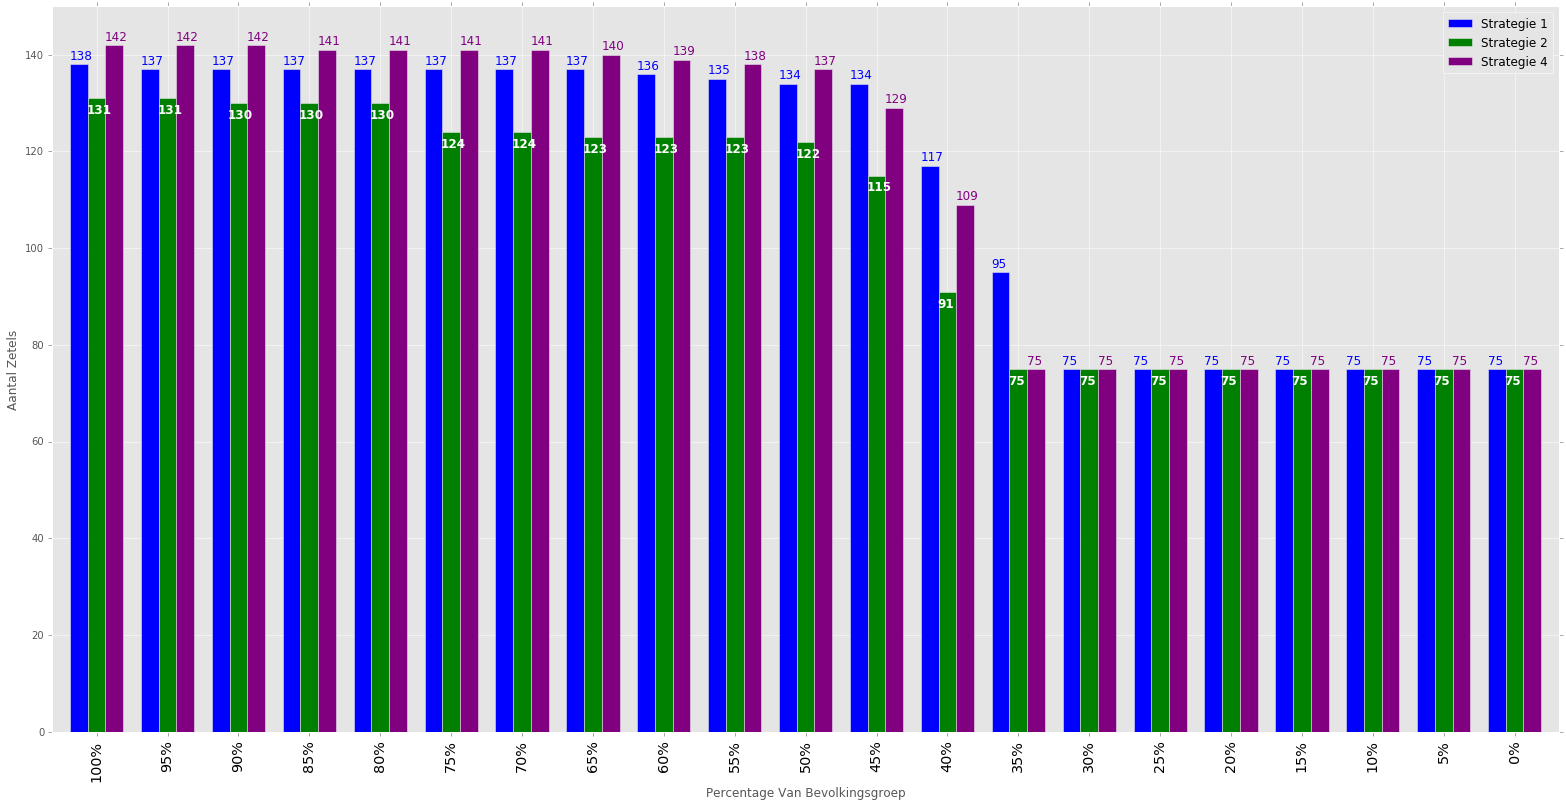
\includegraphics[width=\linewidth]{percentages_van_provincialenS1S2S4.png}

			\caption{Grafiek met overzicht van het maximum aantal zetels wat behaald kon worden wanneer een bepaald percentage van de provinciale kiezers zich committeerde aan strategie 4.}

\label{fig:PerP}
\end{figure}

In Figuur \ref{fig:PerP} is te zien dat wanneer slechts 45\% van de provinciale kiezers zich had gecommitteerd aan strategie 1, er maar vier provinciale kandidaten afgevallen zouden zijn. Bij 35\% van de provinciale kiezers zouden er nog twintig meer provincialen in de Tweede Kamer plaats zouden hebben genomen daadwerkelijk bij de offci\"{e}le verkiezingsuitslag al het geval was (75 provincialen in de Tweede Kamer na offci\"{e}le einduitslag).

Voor strategie 2 is te zien dat bij slechts 50\% van de provinciale kiezers er nog altijd veertig provincialen meer in de Tweede Kamer plaats zouden hebben genomen dan daadwerkelijk bij de offci\"{e}le einduitslag het geval was.

Voor strategie 4 is te zien dat bij slechts 50\% van de provinciale kiezers er nog altijd 62 provincialen meer in de Tweede Kamer plaats zouden hebben genomen dan daadwerkelijk bij de offci\"{e}le einduitslag het geval was. 

 




\paragraph{Tegenstrategie.}
Vanuit de literatuur is er geen directe indicatie te vinden die erop wijst dat er daadwerkelijke anti-provincialen sentimenten bestaan bij Randstedelingen. De literatuur beschrijft wel een gebrek aan een Randstad-identiteit bij inwoners van de Randstad \citep{meijers2001deltametropool,terlouw2010randstad}. Volgens \cite{terlouw2010randstad} echter is het goed mogelijk dat er wel een Randstedelijke identiteit kan ontstaat wanneer er besloten wordt om één grote Randstad-provincie te gaan vormen. Hoewel het vanuit het huidige tijdsbeeld onwaarschijnlijk lijkt dat de Randstedelingen gezamenlijk een (tegen)strategie zullen uitvoeren om te voorkomen dat de provincialen in hogere mate vertegenwoordigd zullen worden in de Tweede Kamer, is het niet onmogelijk dat de Randstedelingen (of een andere groep zoals bijvoorbeeld een groep bestaande uit Randstedelingen én provincialen) op termijn een (tegen)strategie zullen uitvoeren. 



\newpage
\section{Uitvoerbaarheid Strategie\"{e}n}
\label{h6}

\subsection*{Deelvraag 3: Welke strategie is per specifieke bevolkingsgroep aan te bevelen wanneer zij de regel van van voorkeursdrempel in de kieswet te willen benutten in hun voordeel?}
Zoals in het vorige hoofdstuk al is beschreven kunnen de vier verschillende bevolkingsgroepen uit meerdere strate\"{e}n kiezen die een hoog rendement leveren. Daarmee lijkt de derde deelvraag makkelijk te beantwoorden. De bevolkingsgroepen kunnen simpelweg de strategie kiezen waarvan berekend is dat deze het hoogste rendement heeft. Of een strategie de voorkeur geniet boven een andere strategie ligt niet enkel aan het aantal zetels dat een strategie kan opleveren. Echter ligt de keuze voor een strategie ook aan een aantal andere factoren. Zo kan de uitvoering bemoeilijkt worden vanwege de wijze van uitvoering. Een bevolkingsgroep dient als collectief (ook wanneer enkel een deel van de bevolkingsgroep zich committeert) een strategie uit te voeren. Waar sommige Strategie\"{e}n makkelijk communiceerbaar zijn naar het grote publiek zijn andere Strategie\"{e}n moeilijker te communiceren. Echter is het mogelijk om d.m.v. informatie technologie (IT) een hulpmiddel in te schakelen waardoor een strategie nauwelijks gecommuniceerd dient te worden. Enkel het doel geniet dan nog relevantie en niet de wijze waarop het doel precies wordt bereikt. Derhalve zullen we verder kijken dan het rendement wat een strategie voor een bevolkingsgroep oplevert en zullen we de diepte in gaan d.m.v. twee subdeelvragen. \\
\indent In de eerste subdeelvraag gaan we onderzoeken hoe een strategie voor een bevolkingsgroep uitvoerbaar kan worden gemaakt. Hierbij gaan we onderzoeken hoe een strategie te communiceren is. De problematiek van het communiceren van een strategie ligt aan de complexiteit van een strategie. Er kan simpelweg niet verwacht worden dat alle leden van de bevolkingsgroep de regels van de strategie opvolgen wanneer de regels een zekere mate van complexiteit met zich mee brengen. Derhalve zullen we gebruik maken van IT om uitvoering van een strategie te realiseren. In de tweede subdeelvraag gaan we onderzoeken wat de eventuele voor- en nadelen kunnen zijn van de keuze voor de wijze van uitvoering van de strategie. Hierbij zullen we de voor- en nadelen tegen elkaar opwegen om zodoende proberen uit op een aanbeveling voor de wijze van uitvoering van een strategie.  


\subsection{Uitvoeringswijze Strategie\"{e}n.}

\subsection*{Subdeelvraag 3.1: Hoe kan een strategie uitvoerbaar worden gemaakt voor een specifieke bevolkingsgroep waarvan de leden zich willen committeren aan een strategie om de regel van de voorkeursdrempel te willen benutten in hun voordeel?}
In Hoofdstuk \ref{sec:eva} hebben we berekend hoeveel zetels onder leden van een bevolkingsgroep bedeeld hadden kunnen worden wanneer 100\% van de stemgerechtigde leden zich hadden gecommitteerd aan een strategie. In het vorige hoofdstuk hebben we vastgesteld dat zowel strategie 1 als strategie 2 voor elke bevolkingsgroep een hoog rendement oplevert. Echter van deze twee Strategie\"{e}n levert strategie 1, op de bevolkingsgroep allochtonen na, een hoger rendement op. Daarnaast is strategie 1 effici\"{e}nter in het verdelen van de stemmen (zie Hoofdstuk \ref{sec:eva}). Bij de bevolkingsgroep provincialen leverde echter strategie 4 het hoogste rendement op. Zowel strategie 1 als strategie 4 zijn echter moeilijk uit te voeren vanwege het feit dat de stemgerechtigde leden van een bevolkingsgroep op een \textit{N} kandidaten van de corresponderende bevolkingsgroep moeten stemmen. Hierbij wordt de \textit{N} bepaald door een serie aan regels (zie Sectie \ref{vrouwen} voor beschrijving van de regels) en dienen deze regels bekend te zijn bij de deelnemende leden van de bevolkingsgroep. Bij strategie 2 daarentegen moeten de deelnemende leden van de bevolkingsgroep enkel willekeurig op een kandidaat uit de corresponderende bevolkingsgroep stemmen. Bij de bevolkingsgroep vrouwen is dit vrij makkelijk. Op de kandidatenlijst van de partijen staat het geslacht van de kandidaten. Bij de andere bevolkingsgroepen is het echter lastiger om op een willekeurige kandidaat van de corresponderende bevolkingsgroep te stemmen. Op de kandidatenlijsten staat niet of iemand een allochtoon, een oudere of een provinciaal is. De woonplaats van de kandidaat staat niettemin wel vermeld. Echter, wil een provinciale kiezer op een provinciale kandidaat stemmen dan moet de kiezer weten of de woonplaats van de kiezer wel of niet in de Randstad ligt. Het wordt voor de bevolkingsgroepen allochtonen, ouderen en provincialen derha;ve niet alleen moeilijk om strategie 2 out te voeren maar ook om \"{u}berhaupt een strategie uit te voeren. \\
\indent Het uitvoeren en co\"{o}rdineren van strategie 1 bij de bevolkingsgroep vrouwen en het uitvoeren van welke strategie dan ook bij de andere bevolkingsgroepen is dus enigszins problematisch. Vanwege deze problematiek omtrent de uitvoering en co\"{o}rdinatie van de Strategie\"{e}n stellen we een tweetal IT-toepassingen voor. Deze toepassingen kunnen dienen als hulpmiddel voor de kiezers van alle vier de bevolkingsgroepen. Deze tweetal IT-toepassingen kunnen de kiezers assisteren bij het uitvoeren van een strategie. 

\paragraph{Hulpmiddel voor assistentie bij het kiezen van een willekeurige kandidaat.}
We stellen de eerste IT-toepassing voor die dient als hulpmiddel bij het kiezen van een willekeurige kandidaat conform alle in Hoofdstuk \ref{fig:eva} beschreven Strategie\"{e}n (bij alle Strategie\"{e}n moet er uiteindelijk willekeurig op een kandidaat gestemd worden). De toepassing kan al in een vrij simpele vorm bestaan zoals een website en mobiele website maar ook een mobiele applicatie behoort tot de mogeljkheden. Als voorbeeld hebben we echter gekozen voor een website. In Figuur \ref{fig:verkW} is een mock-up van de website te zien. Hierbij moet genoteerd worden dat de mock-up enkel dient om een beeld te scheten van hoe een hulpmiddel in de vorm van een website gebruikt zou kunnen worden. Er is hierbij geen aandacht besteedt aan het ontwerp en de gebruiksvriendelijkheid (usability) van de website. \\
\indent In de mock-up wordt strategie 2 uitgevoerd door de bevolkingsgroep allochtonen. De kiezer kiest de PVDA als de partij waarop zij/hij wilt gaan stemmen en de allochtone kandidaten op de kandidatenlijst van de PVDA worden getoond. De kiezer hoeft nu enkel willekeurig te kiezen uit één van de getoonde allochtone kandidaten. De kiezer kan deze keuze onthouden. Echter is er ook iets te bedenken waardoor de kiezer een reminder zou kunnen ontvangen in de vorm van een sms, een email etc. Het tonen van de foto van de kandidaat is af te raden. Kiezers kunnen op uiterlijk afgaan wanneer zij foto's van de mogelijk te kiezen kandidaten getoond krijgen \citep{banducci2008ballot,lawson2010looking}. \\


\begin{figure}[H]


	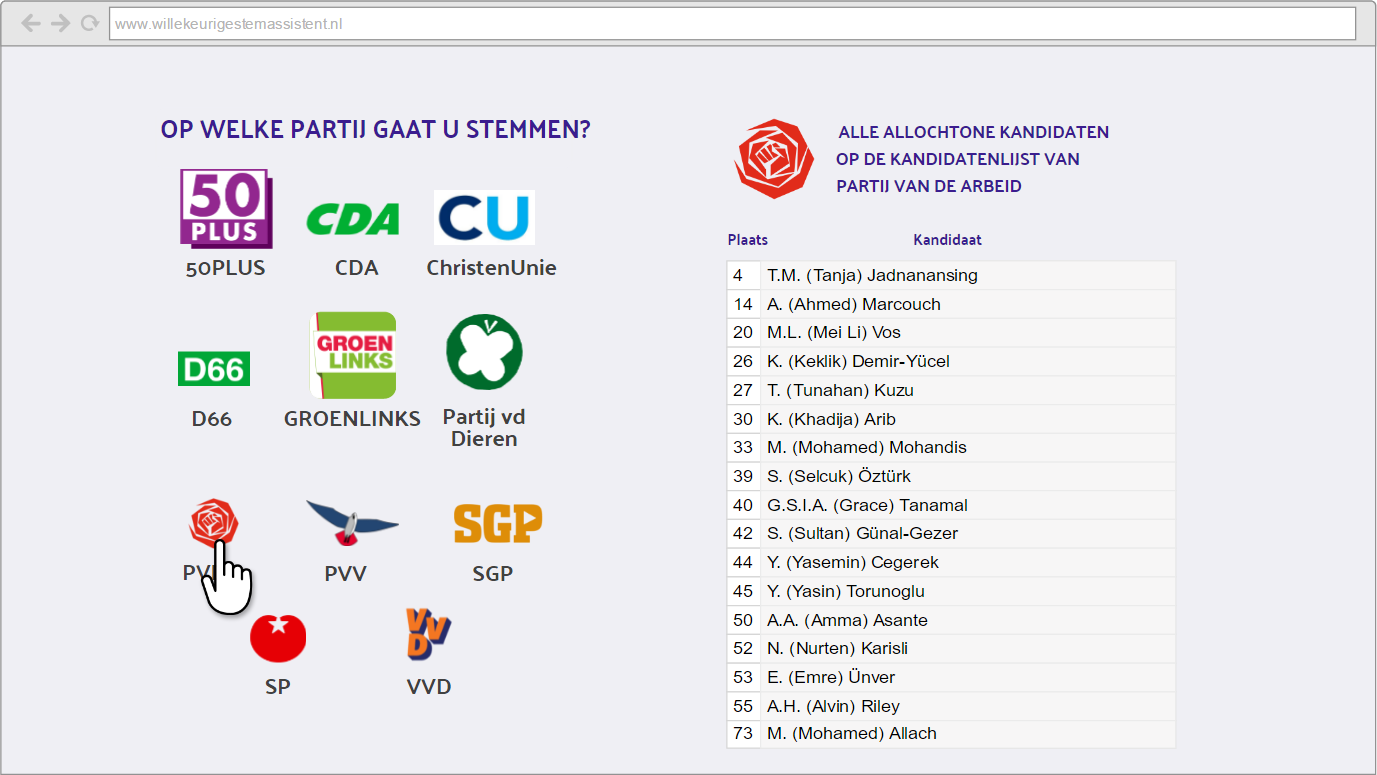
\includegraphics[width=\linewidth]{website_verkiezingen.png}

			\caption{Website als hulpmiddel die deelnemende leden kan helpen bij het kiezen van een willekeurige kandidaat uit de corresponderende bevolkingsgroep. Dit hulpmiddel kan ook bestaan in de vorm van een mobiele website en een mobiele applicatie.}

\label{fig:verkW}
\end{figure}

\paragraph{Hulpmiddel die willekeurige kandidaat uitkiest.}
We stellen de tweede IT-toepassing voor die dient als hulpmiddel bij het kiezen van een willekeurige kandidaat conform alle in Hoofdstuk \ref{fig:eva} beschreven Strategie\"{e}n. Ook deze toepassing kan al in een vrij simpele vorm bestaan zoals een website en mobiele website maar ook een mobiele applicatie behoort tot de mogelijkheden. Als voorbeeld hebben we echter gekozen voor een mobiele applicatie. In Figuur \ref{fig:verkA} is een mock-up van de mobiele applicatie te zien. Ook hierbij moet genoteerd worden dat de mock-up enkel dient om een beeld te scheten van hoe een hulpmiddel in de vorm van een mobiele website gebruikt zou kunnen worden. Er is hierbij geen aandacht besteedt aan het ontwerp en de gebruiksvriendelijkheid (usability) van de mobiele applicatie.\\
\indent In de mock-up wordt een strategie uitgevoerd door de bevolkingsgroep vrouwen. Voor het voorbeeld maakt het niet uit welke strategie dit is aangezien alle Strategie\"{e}n hierbij van toepassing zijn. In de mock-up in Figuur \ref{fig:verkA} kiest de kiezer voor GROENLNKS als de partij waarop zij (kan uiteraard ook een hij zijn als mannelijke kiezers willen deelnemen) wilt gaan stemmen en de mobiele applicatie wijst willekeurig een vrouwelijke kandidaat van GROENLINKS aan waarop de kiezer geacht wordt om de stem op uit te brengen. 


\begin{figure}[H]


	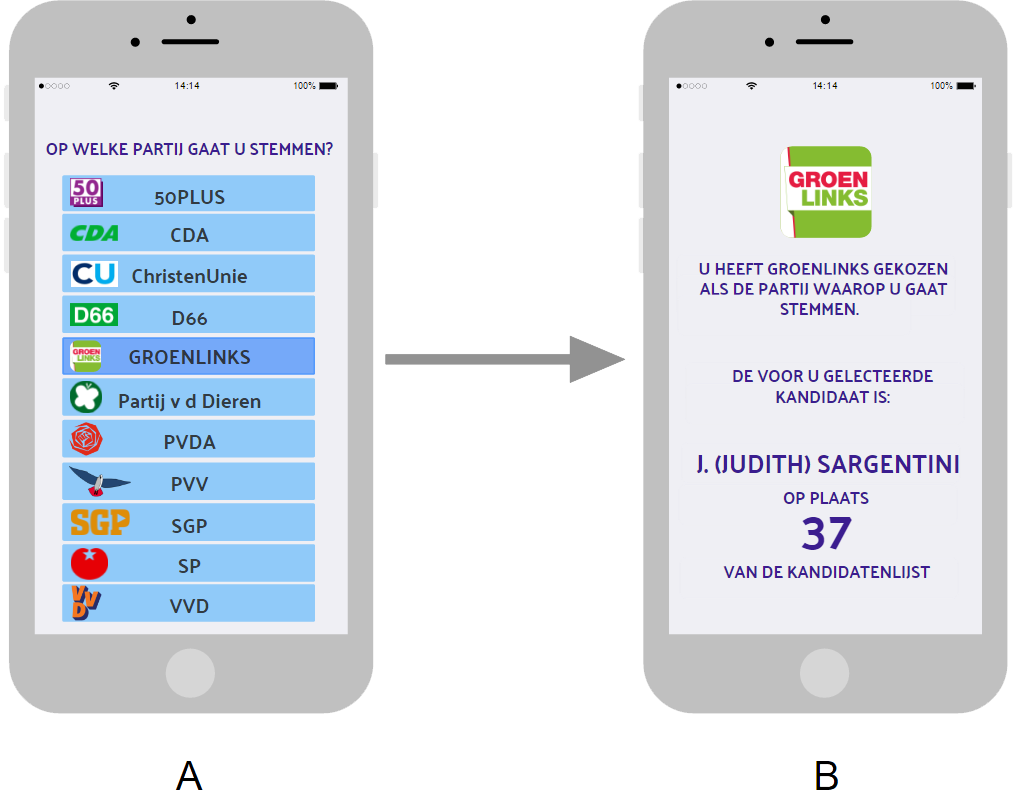
\includegraphics[width=\linewidth]{app_verkiezingen.png}

			\caption{Mobiele applicatie als hulpmiddel die een willekeurige kandidaat uitkiest. Dit hulpmiddel kan ook bestaan in de vorm van een mobiele website en een mobiele applicatie.}

\label{fig:verkA}
\end{figure}

In deze sectie hebben we gepoogd een antwoord te verschaffen op hoe een strategie uitgevoerd zou kunnen worden. Waar strategie 2 voor de bevolkingsgroep vrouwen gemakkelijk uitgevoerd kan worden en geen hulpmiddel aan te pas hoeft te komen, is de strategie voor de andere bevolkingsgroepen moeilijker uit te voeren. Een hulpmiddel in de vorm van een I-toepassing biedt uitkomst. In de volgende sectie gaan we de voor- en nadelen onderzoeken betreffende de keuze voor de wijze waarop een strategie zal worden uitgevoerd. 

\subsection{Voor- en nadelen van keuze voor een uitvoeringswijze strategie.}

\subsection*{Subdeelvraag 3.2: Wat zijn de eventuele voor- en nadelen van de keuze van de wijze waarop een strategie zal worden uitgevoerd?}
In de vorige sectie hebben we een tweetal IT-toepassingen voorgesteld die als hulpmiddel kunnen fungeren bij het uitvoeren van een strategie. Tevens hebben we opgemerkt dat strategie 2 voor de bevolkingsgroep vrouwen vrij gemakkelijk uit te voeren is. In deze sectie zullen we voor- en nadelen gaan onderzoeken van het kiezen voor een bepaalde uitvoeringswijze van een strategie. 

\paragraph{Hulpmiddel en geen hulpmiddel.} 
Vanwege de complexiteit die bij uitvoering van het merendeel van de Strategie\"{e}n om de hoek komt kijken hebben we een tweetal hulpmiddelen voorgesteld in de vorm van IT-toepassingen. Echter is het de vraag of er een behoefte zou zijn bij de deelnemende leden van de bevolkingsgroepen op de hulpmiddelen daadwerkelijk te gaan hanteren. \\
\indent Volgens de \textit{Information Richness Theory} \citep{daft1983information} willen mensen onzekerheid zoveel mogelijk pareren bij het uitvoeren van een taak. Hierbij is o.a. een directe terugkoppeling een belangrijk criteria. Voor uitvoering van alle Strategie\"{e}n is het dus zaak onzekerheid uit te sluiten wat betreft de mogelijke kandidaten waaruit gekozen dient te worden. Enkel bij strategie 2 bij de bevolkingsgroep vrouwen is er een directe terugkoppeling aanwezig om de kandidatenlijst. Bij strategie 2 moeten de kiezers willekeurig een corresponderende kandidaat kiezen en het geslacht van de kandidaat staat op de kandidatenlijst. Zodoende is bij uitvoering van strategie 2 door de bevolkingsgroep vrouwen geen hulpmiddel nodig. Bij de andere Strategie\"{e}n bij deze bevolkingsgroep moet er echter uit een top \textit{N} kandidaat worden gekozen (zie Hoofdstuk \ref{sec:eva}). Voor de andere strategie\"{e}n geldt dat er zowel geen directe terugkoppeling is te vinden op de kandidatenlijst (strategie 2) alsmede regels van de strategie te complex kunnen zijn om gemakkelijk toe te passen. \\
\indent Conform de \textit{Theory of Reasoned Action} \citep{fishbein1977belief,ajzen1991theory} en, in het verlengde van deze theorie, de \textit{Technology Acceptance Model} \citep{davis1989perceived,davis1989user, venkatesh2000determinants} zullen kiezers bereidwillig tegenover het gebruik van de technische hulpmiddelen staan wanneer deze hulpmiddelen de uit te voeren taak makkelijker maakt. Zodoende kan worden aangenomen dat in de meeste gevallen een hulpmiddel gewenst is bij het uitvoeren van een strategie. 

\paragraph{Keuze tussen een online of lokale database voor de mobiele applicatie.}
Wanneer een hulpmiddel in de vorm van een mobiele applicatie wordt gehanteerd zijn er enkele factoren wat betreft de data waar rekening mee gehouden dient te worden. Voor het verkrijgen van de data en de informatie tonen aan de gebruiker van de mobiele applicatie kan gekozen worden tussen een online database en een lokale database. Echter is ook beiden opties een mogelijkheid.  \\
\indent De online database zal een \textit{server/client} \citep{Chapt17:online} connectie opzetten waarbij de client de connectie met de server initieert en er data van de server naar de client en andersom gestuurd kan worden. Dit houdt in dat de gebruiker een internetconnectie dient te hebben om te zorgen dat de gewenste data actueel is en, in het geval van strategie 1 en 4, correspondeert met de laatste peilingen. Ook kan er voor gekozen worden om de keuze van de kiezer bij te houden in de database. Zo kunnen stemmen eventueel effic\"{e}nter gedistribueerd worden over de kandidaten. Echter is dit gevoelig voor manipulatie wanneer een persoon deze functionaliteit wil gebruiken om incorrecte data naar de database te sturen. Tevens is het de vraag of het ethisch verantwoord is om op deze manier bij te houden op welke partij een gebruiker stemt. \\
\indent Tegenover het gebruik van een online database staat het gebruik van een lokale database ge\"{i}mplementeerd in de mobiele applicatie. Voor een lokale database is geen internetconnectie nodig. De database wordt al simpelweg gevuld meegeleverd wanneer de mobiele applicatie wordt ge\"{i}nstalleerd. Een nadeel van een lokale database is echter dat de data in de database eventueel niet actueel is. Peilingen veranderen dagelijks en als een kiezer bijvoorbeeld tien dagen voor de verkiezingen de mobiele applicatie heeft ge\"{i}nstalleerd is de kans groot dat de data niet meer correspondeert met de laatste peilingen. Zodoende worden op de manier strategie 1 en strategie 4 waarschijnlijk niet optimaal uitgevoerd. \\
\indent Zowel een online database als een lokale database brengen voor- en nadelen met zich mee. Echter een combinatie van beiden kan uitkomst bieden. Een online database kan een lokale database vullen met de actuele data. Zodra de mobiele applicatie een internet connectie heeft opgezet kan de lokale database opnieuw opgevuld worden \citep{silberschatz1997database}. Ook in het geval dat de kiezer ten tijden van het gebruiken van de mobiele applicatie tijdens het uitbrengen van de stem geen internetconnectie heeft, kan de laatst opgehaalde data worden getoond aan de kiezer.


\paragraph{Willekeurige keuze van de kiezer vs. willekeurige toewijzing van een kandidaat aan de kiezer.} Bij het eerste voorgestelde hulpmiddel geeft de kiezer aan welke partij zij/hij wilt gaan stemmen waarna er een lijst wordt getoond met mogelijke kandidaten. Herbij wordt er vanuit gegaan dat de kiezer in staat is een willekeurige keuze te maken. Echter is het zo dat de mens inadequaat is als het gaat om willekeurige keuzes maken \cite{schulz2012analysing,bar1991perception,neuringer1986can}. Een computer is d.m.v. het toeassen van een \textit{Pseudorandom Number Generator} (PRNG) veel adequater in het willekeurig kiezen uit bijvoorbeeld een serie getallen of namen \cite{lewis1969pseudo,RANDO99:online,matsumoto1998mersenne,rukhin2001statistical}. Zodoende is het de vraag tot in hoeverre het aan de kiezer kan worden overgelaten om een willekeurige keuze te maken uit een lijst met namen zoals het geval zou zijn bij het gebruik van de eerst voorgesteld hulpmiddel. Bij het tweede voorgestelde hulpmiddel wordt  een kandidaat derhalve geselecteerd door de PRNG. Echter is het de vraag hoe kiezers reageren wanneer zij een kandidaat voorgeschoteld krijgen. Wanneer kiezers deze vorm verwerpen (bijvoorbeeld vanwege het gebrek aan keuzevrijheid) lijkt de eerste vorm voor een hulpmiddel meer geschikt. Hier is daarom aan te bevelen hier verder onderzoek naar te doen wanneer deze hulpmiddelen ontwikkeld gaan worden.  

\iffalse
\subsection{Beantwoording Deelvraag}
In deze sectie komen we nog even kort terug te komen op de deelvraag die in dit hoofdstuk is behandeld. De deelvraag luidde: welke strategie is per specifieke bevolkingsgroep aan te bevelen wanneer zij de regel van van voorkeursdrempel in de kieswet uit willen buiten in hun voordeel? Zoals al eerder gez
\fi
\newpage 
\newpage
\section{Tegenbeweging en de Zoektocht naar het Nash Equilibrium}
\label{h7}

\subsection*{Deelvraag 4: Wat kan er gebeuren wanneer een bevolkingsgroep zich committeert aan een strategie en een andere bevolkingsgroep zich committeert aan een tegenstrategie?}


In Hoofdstuk \ref{sec:eva} hebben we beschreven en berekend hoe bevolkingsgroepen de regel van de voorkeursdrempel in hun voordeel kunnen gebruiken wanneer zij zich gezamenlijk committeren aan een strategie. In dit hoofdstuk gaan we onderzoeken wat er kan gebeuren wanneer een andere bevolkingsgroep zich committeert aan een (tegen)strategie om zodoende zelf een voordeel te kunnen behalen. Hierbij zullen we een hypothetische partij gebruiken die we de \textit{Nash-partij} noemen. In het voorbeeld zijn er twee bevolkingsgroepen: mannelijke kiezers en vrouwelijke kiezers. Interessant is hierbij te onderzoeken of er een \textit{Nash Equilibrium} bereikt kan worden. Een Nash Equilibrium werd voor het eerst beschreven door de Amerikaanse wiskundige en economoon John Forbes Nash Jr. \citeyearpar{nash1950equilibrium} en kan als volgt worden omschreven: een toestand van een systeem met meerdere participanten waarbij geen van de participanten een voordeel kan behalen d.m.v. het veranderen van strategie zolang alle andere participanten oververanderd blijven in hun strategie \citep{christiansen2016neuroeconomics, nashprinceton}. Oftewel is er een toestand te bereiken wanneer het uitvoeren van strategie\"{e}n door twee (of meerdere) bevolkingsgroepen geen extra voordeel meer oplevert wanneer een bevolkingsgroep zijn/haar strategie aanpast maar de andere groep onveranderd blijft? 

\subsubsection*{Aannames.} \label{aannamesNash}
In deze sectie zijn er allereerst een aantal aannames benodigd voordat we kunnen gaan onderzoeken wat er gebeurt wanneer twee (of meerdere) bevolkingsgroepen zich committeren aan een strategie. Ten behoeve van de leesbaarheid en begrijpelijkheid zullen we deze aannames doen om zodoende te gaan onderzoeken of er een Nash Equilibrium bereikt kan worden. Deze aannames zijn:

\begin{itemize}
	\item
In de zoektocht naar het Nash Equilibrium kijken we naar één partij. Deze partij noemen we, als eerbetoon aan John Forbes Nash Jr., de Nash-partij. Voor de Nash-partij geldt:
		\begin{itemize}
			\item
			De partij verwacht het aantal van tien zetels te gaan ontvangen bij de verkiezingen. Het aantal zetels noemen we \textit{Z}. Derhalve geldt voor de Nash-partij $Z=10$
			\item
			Het aantal vrouwelijke en mannelijke kandidaten op de kandidatenlijst van de Nash-partij is gelijk verdeeld met tien om tien. Er staan dus in totaal twintig kandidaten op de kandidatenlijst. 
			\item
			De vrouw-man stemmenverdeling is 60\% om 40\%. Oftewel 60\% van de stemmen op de Nash-partij worden uitgebracht door vrouwelijke kiezers en 40\% van de stemmen op de Nash-partij worden uitgebracht door mannelijke kiezers. Hierbij nemen we \textit{P} als de kans dat een stem op de Nash-partij door een vrouwelijke kiezer wordt uitgebracht en ($1-P$) als de kans dat een stem op de Nash-partij door een mannelijke kiezer wordt uitgebracht. In dit geval geldt dus $P=0,6$ voor de vrouwelijke stemmen en ($1-P)=0,4$ voor de mannelijke stemmen.
			\item
			Zowel 100\% van de vrouwelijke kiezers alsmede 100\% van de mannelijke kiezers die hun stem uitbrengen op de Nash-partij doen mee aan de strategie.
		\end{itemize}
	\item
We stellen een hypothetische verkiezing op. Deze verkiezingen zijn in opzet hetzelfde als de Tweede Kamerverkiezingen in Nederland conform de kieswet \citeyearpar{kieswetje}. Bij deze verkiezingen geldt:
		\begin{itemize}
			\item 
		De kiesdeler is zestig stemmen. Oftewel één zetels staat gelijk aan zestig stemmen.
		\item
		De voorkeursdrempel is dertig stemmen. Een kandidaat heeft dus minstens dertig stemmen nodig om met voorkeur gekozen te worden.
		\end{itemize}
\end{itemize}

\begin{theorem} "De toestand van een Nash Equilibrium wordt bereikt wanneer de verdeling van stemmen \textit{P/(1-P)} op een partij gelijk is aan de verdeling van het aantal zetels (\textit{Z}) voor vrouwelijke en mannelijke kandidaten waarbij geldt dat de zetelverdeling \textit{P*Z/(1-P)*Z} is. Dit is tevens het enige Nash Equilibrium." \\
\end{theorem}

Om de bovenstaande stelling te bevestigen of te ontkrachten zullen we hieronder een aantal voorbeelden schetsen. Zoals hierboven is bepaald, kan de Nash-partij tien zetels (\textit{Z=10}) gaan verwachten. Dit komt neer op het aantal van ($10*60$ = ) 600 stemmen. Van de zeshonderd stemmen op de Nash-partij is de kans $P=0,6$ dat een stem afkomstig van een vrouwelijke kiezer. Dit komt neer op het aantal van ($0,6*600$ = ) 360 stemmen van vrouwelijke kiezers. Het aantal stemmen dat afkomstig is van mannelijke kiezers komt daarmee uit op ($600*(1-P)=600-360$ = ) 240 stemmen.

Het eerste scenario dat we bespreken gaat als volgt: zowel de vrouwelijke als de mannelijke kiezers hanteren dezelfde strategie. Bij deze strategie worden de stemmen willekeurig uitgebracht op één van de eerste tien kandidaten op de kandidatenlijst. Zodoende krijgen de eerste tien vrouwelijke kandidaten op de kandidatenlijst van de Nash-partij het aantal van ($360\div10$ = ) 36 stemmen per kandidaat. De mannelijke kandidaten echter krijgen slechts het aantal van ($240\div10$ = ) 24 stemmen per kandidaat. Vanwege het feit dat de voorkeursdrempel op dertig stemmen is vastgesteld, worden de tien zetels die de Nash-partij ontvangt bedeeld aan tien vrouwelijke kandidaten en is er dus geen enkele mannelijke kandidaat verkozen.

Er vanuit gaande dat de beiden groepen op de hoogte zijn van elkaars strategie, kunnen de mannelijke kiezers hun strategie aanpassen om te voorkomen dat de tien zetels van de Nash-partij aan enkel vrouwelijke kandidaten worden bedeeld. Zo kunnen de mannelijke kiezers de stemmen over de eerste zes kandidaten verdelen in plaats van over de eerste tien. Op deze wijze komen de eerste zes mannelijke kandidaten op het aantal van ($240\div6$ = ) 40 stemmen per kandidaat. Wanneer de vrouwelijke kiezers hun strategie niet aanpassen en derhalve de eerste tien vrouwelijke kandidaten het aantal van 36 stemmen per kandidaat bezorgen, worden er zes zetels aan de mannelijke kandidaten bedeeld en vier zetels aan de vrouwelijke kandidaten bedeeld. 

Wanneer vrouwelijke kiezers er echter wel voor kiezen om hun strategie aan te passen om daarmee een voordeel te behalen, kunnen zij hun stemmen verdelen over de eerste acht vrouwelijke kandidaten van de Nash-partij in plaats van de eerste tien. Op deze wijze komen de eerste acht vrouwelijke kandidaten op het aantal van ($360\div8$ = ) 45 stemmen per kandidaat. Wanneer de mannelijke kiezers hun strategie niet verder aanpassen en derhalve de eerste zes mannelijke kandidaten het aantal van 40 stemmen per kandidaat bezorgen, worden er acht zetels aan vrouwelijke kandidaten bedeeld en twee aan mannelijke kandidaten. 

In Tabel \ref{table:nashtab} is de zien wat er gebeurt wanneer deze ontwikkeling van het aanpassen van de strategie zich doorzet. Daarbij moet genoteerd worden dat elke keer dat een bevolkingsgroep zijn of haar strategie aanpast het zo is dat de andere groep de laatste gekozen strategie hanteert. 


\begin{table}[H]
\centering

		



\iffalse
\begin{tabular}{|r|r|r|r|r|r|}
\hline
V   & M   & V   & M   & V   & M   \\ \hline
6   & 4  & NaN & NaN & NaN & NaN \\ \hline
7   & 3   & 5   & 5 \tikzmark{f}   & NaN & NaN \\ \hline
NaN & NaN & 8   & \tikzmark{d}{2} \tikzmark{e}  & \tikzmark{c}{4}   & \tikzmark{b}{6}   \\ \hline
NaN & NaN & NaN & NaN & 10  & \tikzmark{a}{0}   \\ \hline
\end{tabular}

\begin{tikzpicture}[overlay, remember picture, shorten >=.5pt, shorten <=.5pt]

   \draw [->] ({pic cs:a}) [line width=0.35mm, yshift=-1] to ({pic cs:b});
    \draw [->] ({pic cs:c}) [line width=0.35mm, yshift=-1] to ({pic cs:d});
    \draw [->] ({pic cs:e}) [line width=0.35mm, yshift=-1] to ({pic cs:f});
\end{tikzpicture}
\fi


%\left\Downarrow% Use `\left.` if don't want arrow on this side.
\begin{tabular}{llrr}
\toprule
 {}                                       & {}            & Aantal Zetels & Aantal Zetels \\
 Strategie (op volgorde van aanpassing)                    &                          {}   & Vrouwen       & Mannen \\
\midrule
Beiden bevolkingsgroepen zelfde strategie & \tikzmark{a}{} & 10 &  0\\
Mannelijke kiezers passen strategie aan   &   {}          & 4  &  6 \\
Vrouwelijke kiezers passen strategie aan  &    {}          & 8  &  2\\
Mannelijke kiezers passen strategie aan   &    {}          & 5  &  5 \\
Vrouwelijke kiezers passen strategie aan  &    {}          & 7  &  3 \\
Mannelijke kiezers passen strategie aan   & \tikzmark{b}{} & 6  &  4 \\
\bottomrule
\end{tabular}
%\right.



\begin{tikzpicture}[overlay, remember picture, shorten >=.5pt, shorten <=.5pt]

   \draw [->] ({pic cs:a}) [line width=0.4mm, yshift=2, ] to ({pic cs:b});

\end{tikzpicture}




			\caption{De verdeling van de zetels wanneer één van de twee bevolkingsgroepen de strategie aanpast terwijl de andere groep de laatste gekozen strategie hanteert. Het Nash Equilibrium wordt bereikt bij zes zetels voor de vrouwen en vier zetels voor de mannen.}
\label{table:nashtab} 
\end{table}

Zoals te zien in Tabel \ref{table:nashtab} hierboven toont de onderste rij in de tabel het punt waarop de vrouwelijke kandidaten het aantal van zes zetels hebben ontvangen en de mannelijk kandidaten het aantal van vier zetels hebben ontvangen. Hiermee is volgens de eerdere genoemde stelling het Nash Equilibrium bereikt. De verhouding van de verdeling van het aantal zetels is nu namelijk (\textit{P*Z/(1-P)*Z} = $0,6*10/(1-0,6)*10$ = ) 6/4. Echter is het de vraag of daadwerkelijk het Nash Equilibrium is bereikt. Om te bewijzen dat het Nash Equilibrium daadwerkelijk is bereikt, en dat dit teven het enige Nash Equilibrium is, gaan we nogmaals de strategie van de vrouwelijke en de mannelijk kiezers aanpassen vanuit de laatste rij in Tabel \ref{table:nashtab}. 

In de laatste rij in de tabel hebben de mannelijke kiezers hun stemmen verdeeld over de eerste vier mannelijke op de kandidatenlijst. Op de wijze komen de eerste vier mannelijke kandidaten op het aantal van ($240\div4$ = ) 60 stemmen per kandidaat. De vrouwelijke kiezers bleven daarentegen constant in hun laatst gekozen strategie. Daarbij verdeelden zij de stemmen over zeven vrouwelijke kandidaten. Zodoende kwamen de eerste zeven vrouwelijke kandidaten uit op het aantal van ($360\div7$ = ) 51 stemmen per kandidaat. De eerste vier mannelijke kandidaten hebben dus ($60-51$ = ) 9 stemmen meer per kandidaat. Hierdoor worden de eerste vier zetels bedeeld aan de eerste vier mannelijke kandidaten op de kandidatenlijst en de andere zes zetels worden bedeeld aan de eerste zes vrouwelijke kandidaten op de kandidatenlijst. De vrouwelijke kandidaten hebben immers minder stemmen per kandidaat. 

Mannelijke kiezers kunnen nu ervoor kiezen om hun strategie nogmaals aan te passen en de stemmen te verdelen over de eerste drie mannelijke kandidaten op de kandidatenlijst. Op deze wijze komen de eerste drie mannelijke kandidaten op het aantal van ($240\div3$ = ) 80 stemmen per kandidaat. Echter hebben de overige mannelijke kandidaten geen enkele stem ontvangen. Vanwege het feit dat de eerste zeven vrouwelijke kandidaten 51 stemmen per kandidaten hebben ontvangen, gaan de mannelijke kandidaten er dus op achteruit. Bij de voorlaatste strategie hadden zij immers vier zetels bedeeld gekregen. Bij de laatste strategie zijn dat er nog maar drie zetels.

In het volgende voorbeeld passen de vrouwelijke kiezers hun strategie aan. Daarbij hebben de mannelijke kiezers hun strategie niet aangepast zoals in het laatste voorbeeld hierboven. De mannelijke kiezers verdelen hun stemmen dus over de eerste vier mannelijke kandidaten op de kandidatenlijst. In plaats van dat de vrouwelijke kiezer nu hun stemmen gaan verdelen over de eerste zeven, zoals in hun laatst toegepaste strategie, verdelen zij de stemmen over de eerste zes vrouwelijke kandidaten op de kandidatenlijst. Op deze wijze komen de vrouwelijke kandidaten uit op het aantal van ($360\div6$ = ) 60 stemmen per kandidaat. Zowel de eerste zes vrouwelijke alsmede eerste zes mannelijke kandidaten hebben nu het aantal van 60 stemmen per kandidaat. Daarmee zijn er zes vrouwelijke kandidaten gekozen en vier mannelijke kandidaten. De vrouwelijke kiezers kunnen nu ervoor kiezen om hun strategie nogmaals aan te passen en de stemmen te verdelen over de eerste vijf vrouwelijke kandidaten op de kandidatenlijst. Op deze wijze komen de eerste vijf vrouwelijke kandidaten op het aantal van ($360\div5$ = ) 72 stemmen per kandidaat. Echter hebben de overige vrouwelijke kandidaten geen enkele stem ontvangen. Zodoende worden de eerste vijf zetels van de Nash-partij bedeeld aan de eerste vijf vrouwelijke kandidaten op de kandidatenlijst. Vanwege het feit dat de eerste vier mannelijke kandidaten 60 stemmen per kandidaat hebben ontvangen, worden er vier zetels bedeeld aan mannelijke kandidaten. Er blijft zodoende nog één zetel over. Deze zetel kan voor een mannelijke of vrouwelijke kandidaat zijn. Welke kandidaat deze zetels bedeeld krijgt ligt aan het gegeven of een mannelijke of een vrouwelijke kandidaat op de eerstvolgende plaats op de kandidatenlijst staat die recht geeft op de zetel. Echter in het geval de zetel wordt bedeeld aan een vrouwelijke kandidaat, gaan de vrouwelijke kiezers er niet op vooruit. Zij hadden immers bij de laatste strategie al het aantal van zes zetels behaald en bij deze strategie kunnen zij ook maximaal zes zetels behalen. 

Zodoende is het Nash Equilibrium bereikt bij de zetelverdeling van zes zetels voor vrouwelijke kandidaten en vier zetels voor mannelijke kandidaten. Geen van de bevolkingsgroepen kan erop vooruit wanneer zij hun strategie aanpassen terwijl de andere bevolkingsgroep de strategie niet aanpast. Het punt waarop het Nash Equilibrium wordt bereikt is daarmee tevens het enige Nash Equilibrium. Hierbij moet genoteerd worden dat, hoewel in het voorbeeld twee bevolkingsgroepen zijn gebruikt, het Nash Equilibrium op dezelfde manier ook kan worden bereikt wanneer er meer dan twee bevolkingsgroepen zich committeren aan een strategie. Hierbij geldt dan: $\sum_{b} P{b} * Z = Z$. Oftewel, de som van het aandeel stemmen van de bevolkingsgroepen (\textit{b} staat voor bevolkingsgroep) vermenigvuldigd met het aantal zetels is gelijk aan het totaal aantal zetels.




 

\newpage
\section{Voorkomen Uitbuiting Voorkeursdrempel}
\label{h8}

\subsection*{Deelvraag 5: Hoe kan er voorkomen worden dat de voorkeursdrempel in het voordeel van een bevolkingsgroep kan worden uitgebuit?}

In het vorige hoofdstuk hebben we bewezen dat er een Nash Equilibrium bereikt kan worden wanneer twee bevolkingsgroepen zich beiden committeren aan een strategie. Deze bevolkingsgroepen moeten dan wel op de hoogte zijn van elkaars strategie en daarop inspelen alvorens een Nash Equilibrium kan worden bereikt. In dit hoofdstuk gaan we onderzoeken hoe uitbuiting van de regel van de voorkeursdrempel en daarmee oververtegenwoordiging voorkomen kan worden. Om hier antwoord op te krijgen gebruiken we dezelfde aannames als in het vorige hoofdstuk (zie \hyperref[aannamesNash]{Aannames} in Hoofdstuk \ref{h7}). \\


\begin{theorem}
"De toestand van een Nash Equilibrium wordt direct bereikt wanneer het aantal stemmen dat nodig is voor het behalen van de voorkeursdrempel gelijk is aan de kiesdeler." \\
\end{theorem}

Om de bovenstaande stelling te bevestigen of te ontkrachten zullen we hieronder een aantal voorbeelden schetsen. Hierbij moet genoteerd worden dat we de aannames zoals beschreven in het vorige hoofdstuk (zie \hyperref[aannamesNash]{Aannames} in Hoofdstuk \ref{h7}) op één punt veranderen: de voorkeursdrempel wordt in dit hoofdstuk verhoogd van het aantal van dertig stemmen naar het aantal van zestig stemmen. Daarmee is de voorkeursdrempel gelijk aan de kiesdeler. 

Zoals in het vorige hoofdstuk al is bepaald, kan de Nash-partij tien zetels ($Z=10$) gaan verwachten. Dit komt neer op het aantal van ($10*60$ = ) 600 stemmen. Van de zeshonderd stemmen op de Nash-partij is de kans $P=0,6$ dat een stem afkomstig van een vrouwelijke kiezer. Dit komt neer op het aantal van ($0,6*600$ = ) 360 stemmen van vrouwelijke kiezers. Het aantal stemmen dat afkomstig is van mannelijke kiezers komt daarmee uit op ($600*(1-P)=600-360$ = ) 240 stemmen.

Het scenario dat we gaan bespreken gaat als volgt: zowel de vrouwelijke als de mannelijke kiezers hanteren dezelfde strategie. Bij deze strategie worden de stemmen gedeeld voor de voorkeursdrempel (= 60 stemmen) om zodoende de eerste \textit{N} aantal kandidaten op de kandidatenlijst met corresponderende geslacht aan genoeg stemmen te helpen dat zij de voorkeursdrempel behalen. Op deze wijze krijgen de eerste ($360\div60$ = ) 6 kandidaten op op de kandidatenlijst genoeg stemmen om aan de voorkeursdrempel te voldoen. Bij de mannelijke kandidaten krijgen de eerste ($240\div60$ = ) 4 kandidaten op de kandidatenlijst genoeg stemmen om aan de voorkeursdrempel te voldoen. De overige vrouwelijke mannelijke en vrouwelijke kandidaten op de kandidatenlijst ontvangen geen enkele stem.

Wanneer mannelijke kiezers er voor kiezen om hun strategie aan te passen om daarmee een voordeel te behalen, kunnen zij hun stemmen verdelen over de eerste drie mannelijke kandidaten op de kandidatenlijst. Op deze wijze komen de eerste drie mannelijke kandidaten op het aantal van ($240\div3$ = ) 80 stemmen per kandidaat. De overige mannelijke kandidaten hebben geen enkele stem ontvangen. Vanwege het feit dat de eerste zes vrouwelijke kandidaten het aantal van zestig stemmen per kandidaat hebben ontvangen, zijn er zes vrouwelijke kandidaten en drie mannelijke kandidaten die een zetel bedeeld krijgen. Zodoende blijft er nog één zetels over. Deze zetel kan voor een mannelijke of vrouwelijke kandidaten zijn. Welke kandidaat deze zetels bedeeld krijgt, ligt aan het gegeven of een mannelijke of een vrouwelijke kandidaat op de eerstvolgende plaats op de kandidatenlijst staat die recht geeft op de zetel. Echter in het geval de zetel wordt bedeeld aan een mannelijke kandidaat, gaan de mannelijke kiezers er niet op vooruit. Zij hadden immers bij de initi\"{e}le strategie al het aantal van vier zetels behaald en bij deze strategie kunnen zij ook maximaal vier zetels behalen. 

In het geval de mannelijke kiezers hun strategie niet zouden hebben aangepast en de vrouwelijke kiezers de keuze maken om hun strategie aan te passen, kunnen zij hun stemmen verdelen over de eerste vijf vrouwelijke kandidaten op de kandidatenlijst. Op deze wijze krijgen de eerste vijf vrouwelijke kandidaten op de kandidatenlijst het aantal van ($360\div5$ = ) 72 stemmen per kandidaat. De overige vrouwelijke kandidaten hebben geen enkele stem ontvangen. Zodoende worden de eerste vijf zetels van de Nash-partij bedeeld aan de eerste vijf vrouwelijke kandidaten op de kandidatenlijst. Vanwege het feit dat de eerste vier mannelijke kandidaten 60 stemmen hebben ontvangen per kandidaat, worden er vier zetels bedeeld aan mannelijke kandidaten. Nogmaals blijft er zodoende nog één zetel over. Zoals hierboven al beschreven kan deze zetel voor een mannelijke of vrouwelijke kandidaat zijn. De hoogstgeplaatste kandidaat op de kandidatenlijst zonder stemmen krijgt de zetel bedeeld. Wanneer deze zetel wordt bedeeld aan een vrouwelijke kandidaat, gaan de vrouwelijke kiezers er niet op vooruit. Zij hadden immers bij de initi\"{e}le strategie al het aantal van zes zetels behaald en bij deze strategie kunnen zij ook maximaal zes zetels behalen. 

Zodoende is een Nash Equilibrium direct al bereikt. Ook wanneer beiden partijen een strategie hanteren. De zetelverdeling van zes zetels voor vrouwelijke kandidaten en vier zetels voor mannelijke kandidaten is voor beiden een toestand waaruit ze geen voordeel meer kunnen behalen wanneer zij hun initi\"{e}le strategie aanpassen. Hierdoor is verdere uitbuiting van de voorkeursdrempel niet mogelijk. Het aantal zetels wat een bevolkingsgroep krijgt bedeeld is nu een directe afspiegeling van de verdeling van stemmen van vrouwelijke en mannelijke kiezers op de Nash-partij. 


\paragraph{100\% zekerheid.}
Uit het bovenstaande en het in het vorige hoofdstuk geleverde bewijs kan een regel voor een strategie worden opgesteld die altijd het gewenste rendement zal opleveren ondanks aanpassing van de strategie van de andere bevolkingsgroep(en). Deze regel voor een strategie gaat uit van de volgende aannames:
\begin{itemize}
\item
Alle stemgerechtigden uit de eigen bevolkingsgroep die op de partij willen gaan stemmen doen mee aan de strategie.
\item 
Als bevolkingsgroep zijnde weet je hoeveel de zetels de partij waarop je gaat stemmen zal gaan ontvangen. Daarmee weet je ook het totaal aantal stemmen dat de partij waarop je wil gaan stemmen zal gaan ontvangen.
\item 
Als bevolkingsgroep zijnde weet je het percentage van het totaal aantal stemmen op de partij die afkomstig zijn vanuit de eigen bevolkingsgroep.
\end{itemize}

\noindent Vervolgens luidt de regel: 
\begin{itemize}
\item
De stemmen op de partij afkomstig vanuit de eigen bevolkingsgroep worden willekeurig verdeeld over de top \textit{N} corresponderende kandidaten op de kandidatenlijst van de partij. Hierbij is het top \textit{N} aantal kandidaten een percentage van het totaal aantal te verwachten zetels. Dit percentage is gelijk aan het aandeel stemmen afkomstig vanuit de eigen bevolkingsgroep in verhouding tot het totaal aantal stemmen.
\end{itemize}

Om de hierboven genoemde regel te illustreren nemen we de bevolkingsgroep vrouwen als voorbeeld. Het aantal zetels dat de Nash-partij gaat ontvangen is tien. De stemmen op de Nash-partij zijn verdeeld met 60\% van de stemmen afkomstig van vrouwelijke kiezers en 40\% van de stemmen afkomstig van mannelijke kiezers. Wanneer de vrouwelijke kiezers hun stemmen verdelen over de eerste zes vrouwen op de kandidatenlijst van de Nash-partij krijgen deze vrouwelijke kandidaten met absolute zekerheid het aantal van zes zetels bedeeld, mits de voorkeursdrempel kleiner of gelijk is aan de kiesdeler. Echter lijken de aannames die de regel mogelijk maken niet re\"{e}el. Daarom zullen we in de volgende paragraaf een tweetal adviezen geven die ervoor kunnen zorgen dat een bevolkingsgroep adequater vertegenwoordigd kan worden.

\paragraph*{Adviezen}
In dit hoofdstuk is aangetoond dat de regel van de voorkeursdrempel niet meer is uit te buiten door een bevolkingsgroep wanneer de voorkeursdrempel wordt verhoogd naar hetzelfde aantal stemmen als de kiesdeler. Zodoende kan een bevolkingsgroep niet oververtegenwoordigd zijn wanneer een strategie wordt toegepast. Daarom brengen we het volgende advies uit: om uitbuiting van de regel van de voorkeursdrempel door één of meerdere bevolkingsgroepen te voorkomen, kan de voorkeursdrempel worden verhoogd naar hetzelfde aantal stemmen als het aantal stemmen van de kiesdeler. 

Een tweede advies kan met name een positief gevolg hebben voor de bevolkingsgroep vrouwen. Zoals in Hoofdstuk \ref{h5} al is gesteld lijkt er onder de leden van deze bevolkingsgroep het meeste animo te bestaan voor het uitvoeren van een strategie om zodoende adequater vertegenwoordigd te worden in de Tweede Kamer. Conform de kieswet \citeyearpar{kieswetje} mag het geslacht van de kandidaten op het stemformulier aangeduid worden. Bij de Tweede Kamerverkiezingen van 2012 hadden alle partijen dit ook gedaan \citep{Kiesraad_kandidatenlijsten}. In het geval het eerste advies wordt opgevolgd, luidt het tweede advies als volgt: een eigen stemvakje op het stemformulier voor vrouwelijke kandidaten en een eigen stemvakje voor mannelijke kandidaten. Het is hierbij de bedoeling dat de stemmen op een geslacht worden verdeeld over de top \textit{N} kandidaten op de kandidatenlijst van het corresponderende geslacht. Namelijk, wanneer het eerste advies is opgevolgd en de stemmen niet over de top \textit{N} kandidaten maar over alle kandidaten van het corresponderende geslacht worden verdeeld is het mogelijk dat geen van de kandidaten van dat geslacht boven de voorkeursdrempel komen. Ter illustratie het volgende voorbeeld: vrouwelijke kiezers van de Nash-partij hebben, zoals we weten, 360 stemmen uitgebracht op de partij. Wanneer deze verdeeld worden over de top \textit{N} vrouwelijke kandidaten dat daarmee de voorkeursdrempel kan behalen, zullen er ($360\div60$ = ) 6 vrouwelijke kandidaten een zetels bedeeld krijgen. Echter wanneer de stemmen gelijk verdeeld worden over alle tien de vrouwelijke kandidaten op de kandidatenlijst van de Nash-partij, zullen de vrouwelijke kandidaten, met ($360\div10$ = ) 36 stemmen per kandidaat, allemaal onder de voorkeursdrempel komen. 

Zodoende zullen de stemmen op een geslacht verdeeld dienen te worden over de top \textit{N} kandidaten van het corresponderende geslacht die daarmee de voorkeursdrempel kunnen behalen. Op deze wijze is het aandeel zetels voor kandidaten van een geslacht in verhouding tot het totaal aantal zetels dat de partij ontvangt een directe afspiegeling van de stemverdeling (vrouw-man stemverdeling in het geval van het bovenstaande voorbeeld). Tevens is ook de plaats op de lijst nog altijd van belang. Enkel de top \textit{N} kandidaten van een geslacht zullen een zetel bedeeld krijgen. 

Uiteraard kan op het stemformulier ook worden aangeduid of een kandidaat tot de bevolkingsgroep allochtonen, de bevolkingsgroep ouderen, de bevolkingsgroep provincialen of wat voor bevolkingsgroep dan ook behoort. Verder onderzoek is dan ook nodig om te achterhalen tot in welke mate de verschillende bevolkingsgroepen in Nederland behoefte hebben om adequater vertegenwoordigd te worden in de Tweede Kamer. 



\newpage
\section{Conclusie}
In de Nederlandse Tweede Kamer zijn de bevolkingsgroepen vrouwen, allochtonen, ouderen (personen met een leeftijd van vijftig jaar en ouder) en provincialen (personen die niet in de Randstad wonen) ondervertegenwoordigd. Het aandeel zetels in de Tweede Kamer dat deze groepen bij de laatste Tweede Kamerverkiezingen (2012) hebben ontvangen is geen directe afspiegeling van het aandeel stemgerechtigden afkomstig uit deze bevolkingsgroepen. Vanwege dit feit en vanwege het ontbreken van een enige vorm van quotum bij de Nederlandse politieke partijen zijn er in dit onderzoek een vijfta strate\"{e}n ontwikkeld die de bevolkingsgroepen zouden moeten kunnen helpen om in hogere mate vertegenwoordigd te worden dan bij de einduitslag van de Tweede Kamerverkiezingen in 2012 het geval was. 

Er is aangetoond dat de ontwikkelde strate\"{e}n goed werkten wanneer deze zouden zijn uitgevoerd ten tijde van de Tweede Kamerverkiezingen van 2012. Strategie 1 (top \textit{N} a.d.h.v. de peiling) zou voor alle bevolkingsgroepen een hoog rendement hebben behaald. Bij de bevolkingsgroepen Vrouwen, allochtonen en ouderen zou deze strategie zelfs het hoogste rendement hebben opgeleverd. Strategie 2 (willekeurig stemmen op één van alle kandidaten) zou eveneens voor alle bevolkingsgroepen een hoog rendement hebben opgeleverd. Bij de bevolkingsgroep allochtonen zou het zelfs niets hebben uitgemaakt of strategie 1 of strategie 2 zou zijn uitgevoerd. Beiden zouden hetzelfde aantal zetels voor deze bevolkingsgroep hebben opgeleverd. Tevens is Strategie 2 voor de bevolkingsgroep vrouwen het makkelijkst om uit te voeren. Zij hebben daar geen enkel hulpmiddel bij nodig vanwege het feit dat het geslacht van de kandidaat altijd op het stemformulier vermeld staat. Strategie 4 (top \textit{N+extra percenta}) zou voor de bevolkingsgroep provincialen het hoogste rendement hebben opgeleverd. Strategie 3.1 en strategie 3.2 zouden voor alle bevolkingsgroepen geen hoog rendement hebben opgeleverd en zodoende is het af te raden deze twee strategie\"{e}n ten uitvoer te brengen.

Of het maximum aantal mogelijk kandidaten behaald kan worden ligt een aantal factoren. Om mee te beginnen moeten de partijen waarom een kiezer stemt kandidaten hebben afkomstig uit de bevolkingsgroep van deze kiezer. Ten tijde van de Tweede Kamerverkiezingen van 2012 had de SGP geen vrouwelijke kandidaten en geen allochtone kandidaten op de kandidatenlijst staan. De Partij voor de Dieren had geen allochtonen op de kandidatenlijst staan. Ten tweede dient er vanuit de bevolkingsgroep animo te zijn om zich als collectief (of als substantieel aandeel) achter een strategie te scharen. Afgaande op de bevindingen in Hoofdstuk \ref{h5}, lijkt er bij de bevolkingsgroep vrouwen de meeste animo te zijn voor het uitvoeren van een strategie om zodoende adequater vertegenwoordigd te worden in de Tweede Kamer. Echter, meer onderzoek is nodig bij deze bevolkingsgroep in Nederland om te weten of dit daadwerkelijk zo is. Voor alle groepen geldt dat strategie 1 en strategie 2 bij een deelname van 50\% van de bevolkingsgroep al een substantieel hoger aantal zetels voor de bevolkingsgroepen zou zijn gehaald. Hierbij wordt dan wel aangenomen dat er telkens één bevolkingsgroep een strategie zou hanteren. Ten derde kan het behalen van het maximum uiteraard be\"{i}nvloed worden door de keuze van de strategie. De strategi\"{e} hebben allemaal andere regels voor uitvoering en dit brengt een zeker complexiteit met zich mee. Enkel strategie 2 voor de bevolkingsgroep vrouwen is, zoals hierboven al vermeld, gemakkelijk uit te voeren voor deze bevolkingsgroep.  Ter ondersteuning van het uitvoeren van de strate\"{e}n, hebben we in Hoofdstuk \ref{h6} een tweetal IT-toepassingen voorgesteld. De eerste toepassing toont de kiezer alle uit de eigen bevolkingsgroep afkomstige kandidaten van de partij waar zij/hij op wil gaan stemmen. De kiezer kan dan zelf willekeurig hier een kandidaat uit kiezen. Echter blijkt dat mensen niet adequaat zijn in het willekeurig kiezen. Vandaar dat een een tweede toepassing is voorgesteld. Bij de tweede toepassing geeft de kiezer aan welke partij zij/hij wil gaan stemmen en waarna een willekeurige kandidaat van deze partij wordt toegewezen aan de kiezer.  De tweetal toepassingen dienen slechts als voorstellen en meer onderzoek is dan ook nodig om te bepalen welke functionaliteiten een toepassing daadwerkelijk zou moeten bezitten. De laatste factor die van invloed kan zijn op het behalen van het maximum is een andere bevolkingsgroep (of bevolkingsgroepen) die een (tegen)strategie hanteert. In dit onderzoek is aangetoond dat een Nash Equilibrium kan worden bereikt wanneer twee of meerde groepen zich committeren aan een strategie. Bij \textit{P=percentage stemmen afkomstig uit een bevolkingsgroep in verhouding tot totaal aantal stemmen} en \textit{Z=aantal zetels} geldt: \textit{P*Z/(1-P)*Z} voor een Nash Equilibrium.

Om te voorkomen dat één of meerdere bevolkingsgroepen de voorkeursregel dusdanig uitbuiten dat zij oververtegenwoordigd zijn, hebben we aangetoond dat uitbuiting niet meer mogelijk is bij het verhogen van de voorkeursdrempel van een kwart van het aantal stemmen van de kiesdeler naar het totaal aantal stemmen van de kiesdeler. Bevolkingsgroepen kunnen dan nog altijd een strategie uitvoeren, echter kunnen zij in geen geval beter vertegenwoordigd worden dan de directe afspiegeling van het aandeel stemgerechtigden. Zodoende luidt de eerste aanbeveling van dit onderzoek: om uitbuiting van de regel van de voorkeursdrempel door één of meerdere bevolkingsgroepen te voorkomen, verhoog de voorkeursdrempel naar hetzelfde aantal stemmen als de kiesdeler. 
Zoals hierboven al is vermeld, lijkt er bij de bevolkingsgroep vrouwen waarschijnlijk het meeste animo te bestaan voor het uitvoeren van een strategie. Aangezien het feit dat het geslacht van de kandidaten al op het stemformulier te vinden is en in het geval het eerste advies zal worden opgevolgd doen we ook een tweede advies. Dit advies luidt: een eigen hokje voor vrouwelijke kandidaten en de mannelijk kandidaten. Het is daarbij de bedoeling dat de alle stemmen waarbij het hokje 'vrouwelijke kandidaat' is ingevuld worden verdeeld over alle vrouwen op de kandidatenlijst van de partij. Dit geldt uiteraard ook voor mannelijke kandidaten en hun eigen hokje. In het geval het eerst advies is opgevolgd en alle vrouwelijke kiezers vinken dit hokje aan, wordt het aandeel zetels wat vergeven wordt aan vrouwelijke kandidaten een direct afspiegeling van het aandeel stemmen van vrouwen in verhouding tot het totaal aantal stemmen.

\subsection*{Beperkingen onderzoek.}
Meer onderzoek is nodig naar wat er echt speelt binnen leden van de in dit onderzoek beschreven bevolkingsgroepen. De bevolkingsgroepen vrouwen en daarna allochtonen lijken het meest behoefte te hebben naar een adequatere vertegenwoordiging dan na de Tweede Kamerverkiezingen van 2012 het geval was. Echter is het de vraag in hoeverre leden van deze bevolkingsgroepen zich willen committeren aan een strategie. Daarnaast heeft dit onderzoek met enkele beperking te maken gehad als het ging om de gebruikte data. Zo ontbrak data betreffende peilingen onder de bevolkingsgroepen vrouwen, ouderen en provincialen. Vanwege het ontbreken van deze data, is landelijke peiling gebruikt voor deze bevolkingsgroepen. Hierbij zijn we er van uitgegaan dat de landelijke peiling toereikend was voor deze bevolkingsgroepen. De voorspellingen, wat betreft het aantal stemmen dat een kandidaat volgens de peiling zou gaan ontvangen, geven een beter beeld van de werkelijkheid wanneer elke bevolkingsgroep haar/zijn eigen peiling had. Strategie 1, strategie 2 en strategie 4 zijn op de vier verschillende bevolkingsgroepen getest. Betreffende de Tweede Kamerverkiezingen van 2012 geeft dit voldoende validiteit dat de bevolkingsgroepen in hogere mate vertegenwoordigd zouden zijn geweest wanneer zij een strategie zouden hebben uitgevoerd. Echter door deze drie strateg\"{e}n te uit te testen op eerdere verkiezingen kan met grotere zekerheid worden bepaald of de strate\"{e}n daadwerkelijk toereikend kunnen zijn. Desalniettemin is er vooral één test die de daadwerkelijk kracht van een strategie kan aantonen: de komende Tweede Kamerverkiezingen van 15 maart 2017!


\subsection{Acknowledgements}




























\iffalse
\subsection{Voorkeurstemmen en informatiekunde}
\todo{Hier zou ik bescrijven dat toen je hieraan begon je nog dacht dat er flink wat coordinatie nodig zou zijn om tot een maximaal resultaat te komen. En dat die coordinatie dus allicht met een app uitgevoerd zou kunnen worden. Je was van plan verschillende soorten apps tegen elkaar af te zetten (anoniem of niet, persoonlijk of niet, met een cenrale database of niet, etc etc). Uitiendelijk bleek het zo "gemakkelijk" voor een groep om "de kamer te veroveren" dat coordinatie eigenlijk niet echt nodig was. \\
Je kan nog wel wat speculeren over een lagere en sterk varierende en ook onbekende deelname percentage en hoe een app daar zou kunen helpen}

\subsection{Acknowledgements}
Hier kan je bedanken wie je maar wilt.
\fi


























\newpage



\bibliography{literature}
\bibliographystyle{apacite}
% your refs

%\bibliographystyle{plain}
%\bibliography{MyThesis}

\appendix

\newpage
\section{Bijlage 1}
\label{b1}


\subsection{Bevolkingsgroep: Allochtonen.}
\label{allochtonen}

Betreffende de bevolkingsgroep allochtonen in Nederland worden hieronder de resultaten van de verschillende strategie\"{e}n uiteengezet om zodoende te achterhalen met welke strategie in theorie de meeste allochtone kandidaten in de Tweede Kamer gekozen hadden kunnen worden wanneer alle stemgerechtigde allochtone kiezers in Nederland zich hadden gecommitteerd aan een strategie.\\
\indent In deze sectie worden enkel strategie 1 en strategie 2 toegepast. Strategie 3.1, strategie 3.2 en strategie 4 worden op de bevolkingsgroep allochtonen niet toegepast omdat er te weinig allochtonen op de kandidatenlijsten staan om op de top 15 allochtone kandidaten te stemmen (strategie 3.1) en om voor elke partij een eigen top \textit{N} vast te stellen op basis van aantal allochtone kandidaten (strategie 3.2). Tevens hebben de partijen waar meer allochtone kandidaten op de kandidatenlijst staan dan dat deze partijen aan zetels konden gaan verwachten, te weinig allochtone stemmen ontvangen om een extra percentage aan zetels (voor allochtone kandidaten) bij de \textit{N} toe te voegen (strategie 4).\\
\indent Ten behoeve van de leesbaarheid worden er geen voorbeelden gegeven betreffende berekeningen. Alle voorbeelden zijn te vertalen vanuit de bij de bevolkingsgroep vrouwen toegepaste strategie\"{e}n (zie Sectie \ref{vrouwen}). 

\paragraph{Aannames en Regels.}
De aannames en regels zijn hetzelfde als bij de strategie\"{e}n voor de bevolkingsgroep vrouwen . Hierbij moet genoteerd worden dat vrouwen vervangen dient te worden voor allochtonen en vrouwelijke kandidaten vervangen dient te worden voor allochtone kandidaten (voor een gedetailleerde omschrijving van de aannames zie Sectie \hyperref[besS]{Beschrijving Strategie\"{e}n} en voor de regels van een strategie zie correspondeerde strategie in Sectie \ref{vrouwen}).

\paragraph{Het berekenen van het aantal te verwachten allochtone stemmen.}
Op 1 september 2012 waren er 2.629.699 allochtonen boven de 18 jaar wonenden in Nederland \citep{CBS_allochtonen}. We gaan er voor deze bevolkingsgroep vanuit dat al deze personen stemgerechtigd waren tijdens de Tweede Kamerverkiezingen van 2012. De peiling onder allochtonen \citep{Opiniehuis} gaf aan dat 55\% van de allochtonen zou gaan stemmen. Dat komt neer op (55\%*2.629.699 = ) 1.446.334 stemmen. Op een vergelijkbare wijze als bij de bevolkingsgroep vrouwen, is voor de bevolkingsgroep allochtonen berekend hoeveel stemmen de partijen van allochtone kiezers konden gaan verwachten. Hierbij is het allochtoon stempercentage het percentage van alle door allochtonen uitgebrachte stemmen. Ter illustratie nemen we GROENLINKS als voorbeeld. \\
\indent Volgens de peiling zou GROENLINKS 2,1\% van de allochtone stemmen krijgen. Zoals eerder al berekend, is het aantal stemgerechtigde allochtonen dat gaat stemmen een aantal van 1.446.334. Daarmee komt GROENLINKS op een aantal van ($2,1\%*1.446.334$ = ) 30.373 allochtone stemmen. In Tabel \ref{table:tab1A} hieronder is per partij het allochtone stempercentage te zien evenals het aantal stemmen de partij zou gaan ontvangen van allochtone kiezers.  

\begin{table}[H]
\centering
	\begin{footnotesize}
		\begin{tabular}{lrr}
\toprule
 &  Allochtone Stempercentage  &  Aantal Stemmen Van Allochtonen \\
Partij                &                        &                                 \\
\midrule
50PLUS                &                 0,0 &                               0 \\
CDA                   &                 2,1 &                           30.373 \\
ChristenUnie          &                 0,2 &                            2.893 \\
D66                   &                 7,6 &                          109.921 \\
GROENLINKS            &                 2,5 &                           36.158 \\
Partij v d Dieren &                 0,6 &                            8.678 \\
PVDA                  &                40,9 &                          591.551 \\
PVV                   &                4,7 &                           67.978 \\
SGP                   &                 0,0 &                               0 \\
SP                    &                19,1 &                          276.250 \\
VVD                   &                4,7 &                           67.978 \\
Weet Niet		      & 				17,6 & 						254.555 \\
\midrule
Totaal				&					100	&						1.446.334\\
\bottomrule
\end{tabular}

	\end{footnotesize}
			\caption{Het allochtone stempercentage en het totaal aantal te verwachten allochtone stemmen volgens de peiling.}
\label{table:tab1A} 
\end{table}


\paragraph{Het berekenen van het daadwerkelijke aantal allochtone stemmen.}
De opkomst onder allochtonen lag aanzienlijk hoger dan de peiling van Opiniehuis \citeyearpar{Opiniehuis} had aangegeven met 55\% volgens de peiling om 66\% volgens het CBS \citeyearpar{CBS_stemgedrag}. Er zijn dus meer stemmen door allochtonen uitgebracht dan werd verwacht. Het aantal uitgebrachte allochtone stemmen komt hiermee op ($66\%*2.629.699$ = ) 1.736.055 stemmen. Daarnaast zat de peiling van Opiniehuis er bij een aantal partijen flink naast.  Hieronder is in Tabel \ref{table:tab2A} per partij te zien hoeveel procent van de allochtonen kiezers op de partij heeft gestemd en het aantal stemmen dat een partij van allochtonen heeft ontvangen. Op dezelfde wijze als het berekenen van het aantal te verwachten allochtone stemmen in de vorige paragraaf, is ook het daadwerkelijke aantal allochtone stemmen per partij berekend.
    
\begin{table}[h]
\centering
	\begin{footnotesize}
		\begin{tabular}{lrr}
\toprule
{} &  Allochtone Stempercentage &  Aantal Allochtone Stemmen \\
Partij                &                            &                            \\
\midrule
50PLUS                &                       1,27 &                      22045 \\
CDA                   &                       3,80 &                      65963 \\
ChristenUnie          &                       3,05 &                      52944 \\
D66                   &                       8,32 &                     144425 \\
GROENLINKS            &                       2,30 &                      39925 \\
Partij voor de Dieren &                       1,27 &                      22045 \\
PVDA                  &                      40,83 &                     708936 \\
PVV                   &                       8,31 &                     144252 \\
SGP                   &                       1,27 &                      22045 \\
SP                    &                       9,09 &                     157792 \\
VVD                   &                      20,49 &                     355683 \\
\midrule
Totaal				& 						100 & 			1736055 \\
\bottomrule
\end{tabular}



	\end{footnotesize}
			\caption{Totaal aantal stemmen dat een partij heeft ontvangen, het aandeel stemmen van allochtonen in percentage en het totaal aantal allochtone stemmen volgens de einduitslag.}
\label{table:tab2A} 
\end{table}
    

\subsubsection{Strategie 1: Allochtone kiezers stemmen op top \textit{N} allochtone kandidaten.} \label{S1A}



\paragraph{Verdelingen zetels en aantal allochtone kandidaten.}
In de grafiek hieronder in Figuur \ref{fig:zetelsA} is te zien dat voor alle partijen links van de stippellijn de top \textit{N} gelijk is aan het aantal allochtonen dat de partij op de kandidatenlijst had staan. Bij de partijen rechts van de stippellijn is \textit{N} gelijk aan het aantal te verwachten zetels volgens de peiling. 
 
\begin{figure}[H]

	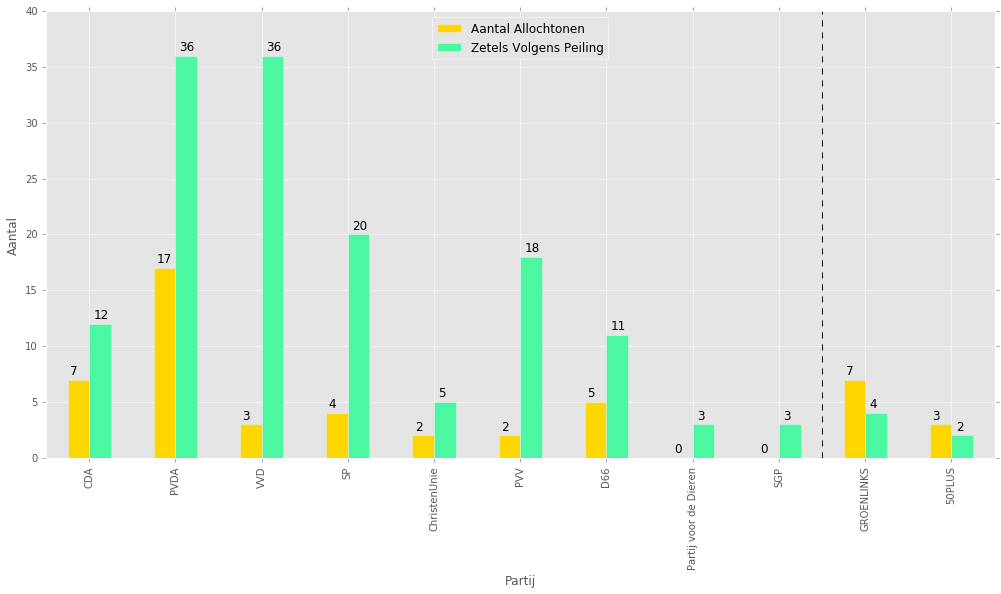
\includegraphics[width=\linewidth]	{Aantal_allochtonen_aantal_zetels1.png}

			\caption{Het aantal allochtonen op de kandidatenlijst(geel) en het aantal zetels volgens de peilingen(groen) per partij.}

\label{fig:zetelsA}
\end{figure}


\paragraph{Maximaal aantal allochtonen per partij (top \textit{N}) dat in de Tweede Kamer gekozen had kunnen worden.}
In Tabel \ref{table:tab3A} hieronder is, in het verlengde van Figuur \ref{fig:zetelsA} hierboven, te zien hoeveel allochtone kandidaten er per partij maximaal in de Tweede Kamer gekozen hadden kunnen worden. In de Tabel is dus per partij het aantal (\textit{N}) allochtone kandidaten te zien waarover de stemmen van de allochtone kiezers op de partij verdeeld zullen worden.  

Vanwege het feit dat de SGP en de Partij voor de Dieren helemaal geen allochtone kandidaten op de kandidatenlijst hadden staan en alle partijen volgens de peiling, op GROENLINKS en 50PLUS na, meer zetels zouden gaan ontvangen dan dat zij allochtone kandidaten op de kandidatenlijsten hadden staan komt het totaal aantal allochtone kandidaten dat volgens de peiling in de Tweede Kamer gekozen had kunnen worden uit op 46. 





\begin{table}[H]
\centering
	\begin{footnotesize}
		\begin{tabular}{lrr}
\toprule
{} &  Top N Allochtone Kandidaten &  Overgebleven Autochtone Kandidaten \\
Partij                &                              &                                     \\
\midrule
50PLUS                &                            2 &                                   0 \\
CDA                   &                            7 &                                   5 \\
ChristenUnie          &                            2 &                                   3 \\
D66                   &                            5 &                                   6 \\
GROENLINKS            &                            4 &                                   0 \\
Partij voor de Dieren &                            0 &                                   3 \\
PVDA                  &                           17 &                                  19 \\
PVV                   &                            2 &                                  16 \\
SGP                   &                            0 &                                   3 \\
SP                    &                            4 &                                  16 \\
VVD                   &                            3 &                                  33 \\
\midrule
Totaal                &                           46 &                                 104 \\
\bottomrule
\end{tabular}

	\end{footnotesize}
			\caption{Per partij de top \textit{N} allochtone kandidaten en de overgebleven autochtone kandidaten a.d.h.v. de peiling.}
\label{table:tab3A} 
\end{table}



\paragraph{Het toewijzen van de stemmen aan de allochtone kandidaten op basis van de peiling en de einduitslag.}
Op dezelfde wijze als bij de andere strategie\"{e}n wijzen we de hier de allochtone stemmen toe a.d.h.v. de peiling en a.d.h.v. de einduitslag (voor gedetailleerde uitleg zie \hyperref[S1V]{Strategie 1}in \hyperref[vrouwen]{Bevolkingsgroep: Vrouwen}). In Figuur \ref{fig:stemmenS1A} hieronder is zowel de toewijzing op basis van de peiling alsmede de toewijzing op basis van de einduitslag te zien.





\begin{figure}[H]

	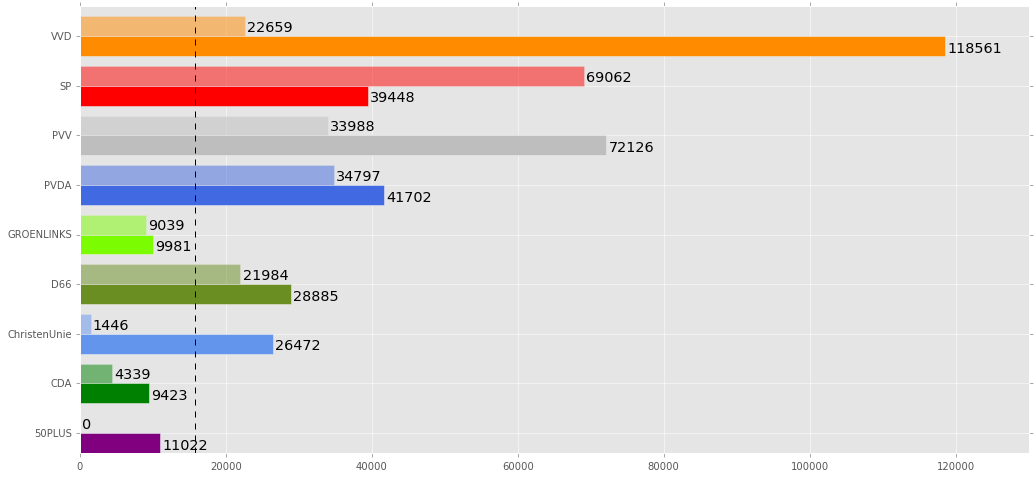
\includegraphics[width=\linewidth]	{stemmen_op_allochtonen_topN_samen2.png}

			\caption{Grafiek met per partij de verdeling van de stemmen van allochtone kiezers op de top \textit{N} allochtone kandidaten van de partij a.d.h.v. de peiling \citep{Opiniehuis} in de licht gekleurd staven en a.d.h.v. de einduitslag \citep{Kiesraad_databank} in de donker gekleurde staven. De stippellijn is de daadwerkelijk voorkeursdrempel(15.708 stemmen).}

\label{fig:stemmenS1A}
\end{figure}


Zoals te zien in Figuur \ref{fig:stemmenS1A} hierboven, zijn bij het toewijzen van de stemmen er enige inconsistenties tussen de voorspelling op basis van de peiling en de einduitslag. Dit kom voornamelijk vanwege het feit dat de peiling onder allochtonen van het Opiniehuis \citeyearpar{Opiniehuis} flink afweek van de werkelijkheid. Echter is de voorspelling a.d.h.v. de peiling grotendeels correct in het voorspellen van welke partijen de allochtone kandidaten boven de voorkeursdrempel gekomen zouden zijn. Alleen wat betreft de ChristenUnie was de voorspelling niet toereikend.

\paragraph{Aantal allochtonen na strategie 1.}
Na het uitvoeren van de strategie 1 en het opstellen van de Tweede Kamer zoals eerder in dit hoofdstuk beschreven, zou strategie 1 een Tweede Kamer hebben opgeleverd op waarin 34 allochtonen en 116 autochtonen hadden plaatsgenomen. Daarmee zouden allochtonen ruim in betere mate vertegenwoordigd zijn geweest dan daadwerkelijk bij de einduitslag van 2012 (dertien zetels bij einduitslag van 2012) het geval was. In de cirkeldiagram in Figuur \ref{fig:pcS1A} hieronder is de verdeling goed te zien. 

\begin{figure}[H]
\centering
	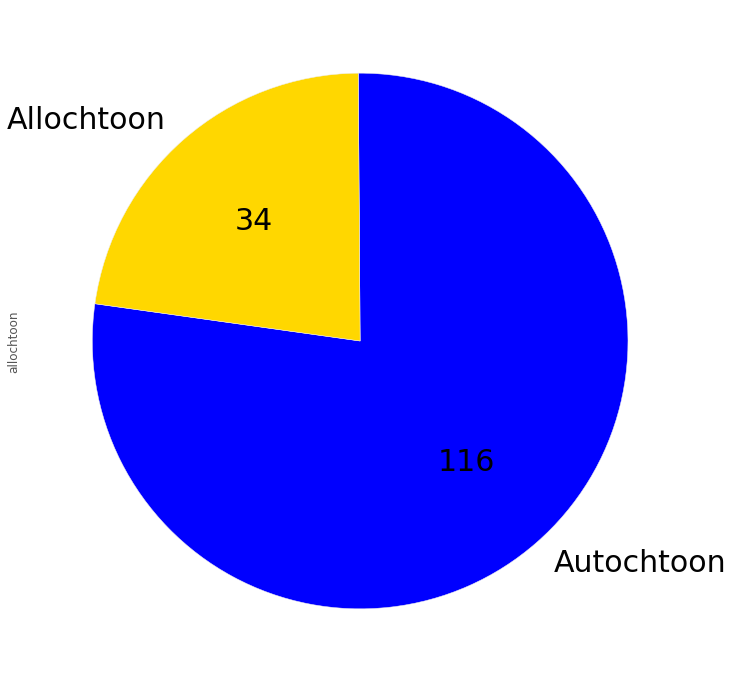
\includegraphics[width=0.33\linewidth]{pie_chart_topN_allochtonen.png}

			\caption{Na uitvoering van de strategie nemen er 34 allochtonen(23\%) en 116 autochtonen(77\%) plaats in de Tweede Kamer.} 

\label{fig:pcS1A}
\end{figure}

\paragraph{Minder dan 46 allochtonen in de Tweede Kamer na uitvoering van strategie 1.}
De reden dat er niet 46 vrouwen maar 'slechts' 34 allochtonen in de Tweede Kamer plaatsnemen na uitvoering van strategie 1 ligt ten grondslag aan een aantal factoren. Bij de ChristenUnie, D66, de PVDA, de PVV, de SP en de VVD zouden alle allochtone kandidaten boven de voorkeursdrempel gekomen zijn en hebben daarmee een zetel hebben gekregen. Deze partijen samen zouden goed zijn geweest voor 33 door allochtonen verkregen zetels. De andere partijen had niet genoeg allochtone stemmen ontvangen om de top \textit{N} allochtone kandidaten boven de voorkeursdrempel te helpen. Hierdoor zouden er in totaal 12 allochtone kandidaten afgevallen zijn. Echter had GROENLINKS, in de persoon van Jesse Klaver, toevallig een allochtone kandidaat die vanwege zijn plaatst op de kandidatenlijst toch een zetels had gekregen.
Het totaal aantal allochtonen in de Tweede Kamer na uitvoering van strategie 1 komt daarom uit op ($46-12$ = ) 34. 


\subsubsection{Strategie 2: Allochtone kiezers stemmen op een willekeurige allochtone kandidaat.}





\paragraph{Het toewijzen van de stemmen aan de allochtone kandidaten op basis van de peiling en de einduitslag.}
Op dezelfde wijze als bij de andere strategie\"{e}n wijzen we de hier de allochtone stemmen toe a.d.h.v. de peiling en a.d.h.v. de einduitslag (voor gedetailleerde uitleg zie \hyperref[S1V]{Strategie 1 }in \hyperref[vrouwen]{Bevolkingsgroep: Vrouwen}). In Figuur \ref{fig:stemmenS2A} hieronder is zowel de toewijzing op basis van de peiling alsmede de toewijzing op basis van de einduitslag te zien.
 


\begin{figure}[H]

	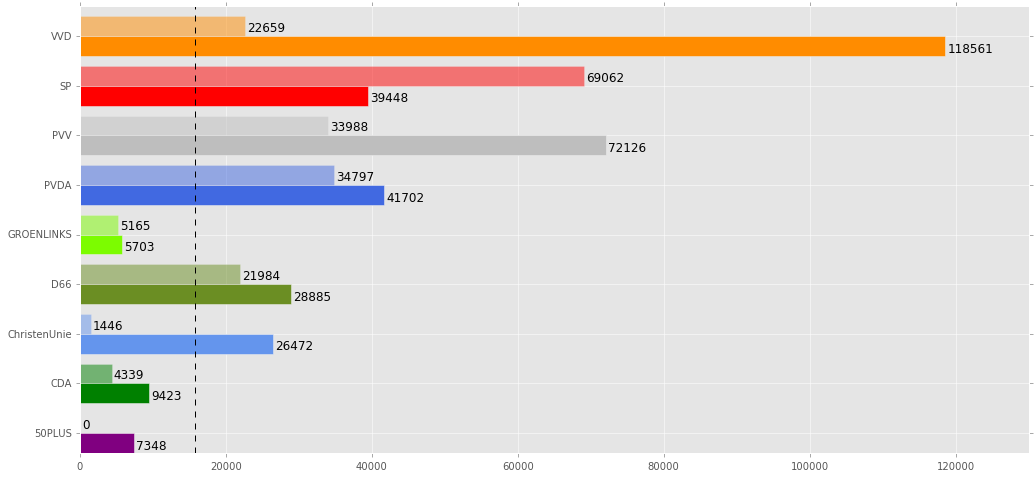
\includegraphics[width=\linewidth]	{stemmen_op_allochtonen_willekeurig_samen2.png}

			\caption{Grafiek met per partij de verdeling van de stemmen van allochtone kiezers op alle allochtone kandidaten van de partij a.d.h.v. de peiling \citep{Opiniehuis} in de licht gekleurd staven en a.d.h.v. de einduitslag \citep{Kiesraad_databank} in de donker gekleurde staven. De stippellijn is de daadwerkelijk voorkeursdrempel(15.708 stemmen).}

\label{fig:stemmenS2A}
\end{figure}

Net zoals bij strategie 1 het geval was en zoals te zien in Figuur \ref{fig:stemmenS2A} hierboven, zijn bij het toewijzen van de stemmen er enige inconsistenties tussen de voorspelling op basis van de peiling en de einduitslag (Zie \hyperref[S1A]{strategie 1} in Sectie \ref{allochtonen} voor verklaring).

\paragraph{Aantal allochtonen na strategie 2.}
Na het uitvoeren van de strategie 2 en het opstellen van de Tweede Kamer zoals eerder in dit hoofdstuk beschreven, zou strategie 2 een Tweede Kamer hebben opgeleverd waarin 34 allochtonen (23\%) en 116 autochtonen (77\%) zouden hebben plaatsgenomen. Daarmee zouden allochtonen ruim in betere mate vertegenwoordigd zijn geweest dan daadwerkelijk bij de einduitslag van 2012 (dertien zetels bij einduitslag van 2012) het geval was. In de cirkeldiagram in Figuur \ref{fig:pcS2A} hieronder is de verdeling goed te zien. 


\begin{figure}[H]
\centering
	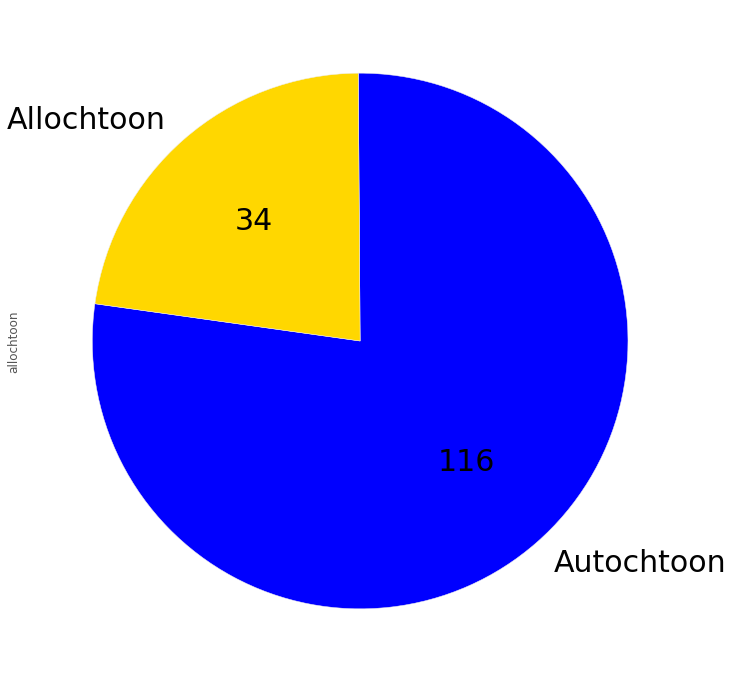
\includegraphics[width=0.35\linewidth]{pie_chart_topN_allochtonen.png}

			\caption{Na uitvoering van de strategie nemen er 34 allochtonen(23\%) en 116 autochtonen(77\%) plaats in de Tweede Kamer.}

\label{fig:pcS2A}
\end{figure}


\paragraph{Hetzelfde aantal allochtonen in de Tweede Kamer als bij strategie 1.}
De reden dat er precies hetzelfde aantal allochtonen in de Tweede Kamer worden gekozen bij strategie 2 ten opzicht van strategie 1 ligt ten grondslag aan een aantal factoren. Zoals het geval is bij strategie 1, zouden bij de ChristenUnie, D66, de PVDA, de PVV, de SP en de VVD alle allochtone kandidaten boven de voorkeursdrempel uitgekomen zijn Dit komt neer op een aantal van 33 door allochtonen verkregen zetels. Daarnaast zouden de overige partijen, net als bij strategie 1, niet genoeg allochtone stemmen hebben ontvangen om de allochtone kandidaten aan de voorkeursdrempel te helpen. De 34e zetel voor een allochtoon was, net als bij strategie 1, Jesse Klaver. Echter heeft hij een zetels verkregen op basis van zijn plaats op de kandidatenlijst. 



\subsection{Bevolkingsgroep: Ouderen.} \label{ouderen}

Betreffende de bevolkingsgroep ouderen in Nederland worden hieronder de resultaten van de verschillende strategie\"{e}n uiteengezet om zodoende te achterhalen met welke strategie in theorie de meeste oudere kandidaten in de Tweede Kamer gekozen kunnen worden wanneer alle stemgerechtigde ouderen kiezers in Nederland zich committeren aan de strategie.\\
\indent Ten behoeve van de leesbaarheid worden er geen voorbeelden gegeven betreffende berekeningen. Alle voorbeelden zijn te vertalen vanuit de bij de bevolkingsgroep vrouwen toegepaste strategie\"{e}n (zie Sectie \ref{vrouwen}). 

\paragraph{Aannames en Regels.}
De aannames en regels zijn hetzelfde als bij de strategie\"{e}n voor de bevolkingsgroep vrouwen . Hierbij moet genoteerd worden dat vrouwen vervangen dient te worden voor ouderen en vrouwelijke kandidaten vervangen dient te worden voor oudere kandidaten (voor een gedetailleerde omschrijving van de aannames zie Sectie \hyperref[besS]{Bescrijving Strategie\"{e}n} en voor de regels van een strategie zie correspondeerde strategie in Sectie \ref{vrouwen}).

\paragraph{Het berekenen van het aantal te verwachten ouderen stemmen.}
Op 1 september 2012 waren er 6.189.591 ouderen (boven de 50 jaar) wonenden in Nederland(CBS, 2012). We gaan er voor deze bevolkingsgroep vanuit dat al deze personen stemgerechtigd waren tijdens de Tweede Kamerverkiezingen van 2012. Vanwege het ontbreken van een peiling onder de oudere kiezers nemen we aan dat de ouderen kiezers hetzelfde stemgedrag vertonen als de Nederlandse kiezers vertoonden volgens de landelijke peiling. We gaan derhalve uit van een opkomst van 73\% (zoals de landelijke peiling aangaf). Dat komt neer op een aantal van (73\%*6.189.591 = ) 4.518.401 stemmen. Op dezelfde wijze als bij de bevolkingsgroep allochtonen, is voor de bevolkingsgroep ouderen berekend hoeveel stemmen de partijen van oudere kiezers konden gaan verwachten (zie Sectie \ref{allochtonen} voor uitleg) . In Tabel \ref{table:tab1O} hieronder is per partij te zien hoeveel procent van de oudere kiezers op een partij heeft gestemd en het aantal stemmen dat een partij van ouderen heeft ontvangen.


\begin{table}[H]
\centering
	\begin{footnotesize}
		\begin{tabular}{lrr}
\toprule
{} &  Oudere Stempercentage &  Aantal Stemmen Van Ouderen \\
Partij                &                        &                             \\
\midrule
50PLUS                &                   1,33 &                       60245 \\
CDA                   &                   8,00 &                      361472 \\
ChristenUnie          &                   3,33 &                      150613 \\
D66                   &                   7,33 &                      331349 \\
GROENLINKS            &                   2,67 &                      120490 \\
Partij voor de Dieren &                   2,00 &                       90368 \\
PVDA                  &                  24,00 &                     1084416 \\
PVV                   &                  12,00 &                      542208 \\
SGP                   &                   2,00 &                       90368 \\
SP                    &                  13,34 &                      602456 \\
VVD                   &                  24,00 &                     1084416 \\
\midrule
Totaal				&				100		&						4.518.401\\
\bottomrule
\end{tabular}

	\end{footnotesize}
			\caption{Totaal aantal stemmen dat een partij zou gaan ontvangen en het totaal aantal te verwachten oudere stemmen volgens de peiling.}
\label{table:tab1O} 
\end{table}


\paragraph{Het berekenen van het daadwerkelijke aantal oudere stemmen.}
Vanwege het ontbreken een peiling onder ouderen was er ook geen prognose over de verwachte opkomst. Daarom hebben we de landelijke opkomstprognose van 73\% genomen. Echter was er een opkomst van 75\% onder de ouderen (CBS). Het aantal uitgebrachte oudere stemmen komt hiermee op ($75\%*6.189.591$ = ) 4.642.193 stemmen. Hieronder in Tabel \ref{table:tab2O} is per partij te zien hoeveel procent van de oudere kiezers op de partij heeft gestemd en het aantal stemmen dat een partij van ouderen heeft ontvangen. Op dezelfde wijze als het berekenen aantal te verwachten allochtone stemmen (zie \hyperref[S1A]{strategie 1} in Sectie \ref{allochtonen}), is ook het daadwerkelijk aantal oudere stemmen per partij berekend. 
    
\begin{table}[h]
\centering
	\begin{footnotesize}
		\begin{tabular}{lrr}
\toprule
{} &  Ouderen Stempercentage &  Aantal Ouderen Stemmen \\
Partij                &                         &                         \\
\midrule
50PLUS                &                    4,00 &                  185687 \\
CDA                   &                    8,00 &                  371375 \\
ChristenUnie          &                    2,67 &                  123792 \\
D66                   &                    8,00 &                  371375 \\
GROENLINKS            &                    2,67 &                  123792 \\
Partij v d Dieren &                    1,33 &                   61895 \\
PVDA                  &                   25,33 &                 1176022 \\
PVV                   &                   10,67 &                  495169 \\
SGP                   &                    1,33 &                   61895 \\
SP                    &                    9,33 &                  433271 \\
VVD                   &                   26,67 &                 1237920 \\
\midrule
Totaal                &                     100 &				4.642.193 \\
\bottomrule
\end{tabular}

	\end{footnotesize}
			\caption{Totaal aantal stemmen dat een partij heeft ontvangen, het aandeel stemmen van ouderen in percentage en het totaal aantal ouderen stemmen volgens de einduitslag.}
\label{table:tab2O} 
\end{table}
    

\subsubsection{Strategie 1: Oudere kiezers stemmen op top \textit{N} ouderen kandidaten.} 

 
\paragraph{Verdelingen zetels en aantal oudere kandidaten.}
In de grafiek hieronder in Figuur \ref{fig:zetelsO} is te zien dat voor alle partijen links van de stippellijn de top \textit{N} gelijk is aan het aantal ouderen dat de partij op de kandidatenlijst had staan. Bij de partijen rechts van de stippellijn is \textit{N} gelijk aan het aantal te verwachten zetels volgens de peiling. 

 
\begin{figure}[H]

	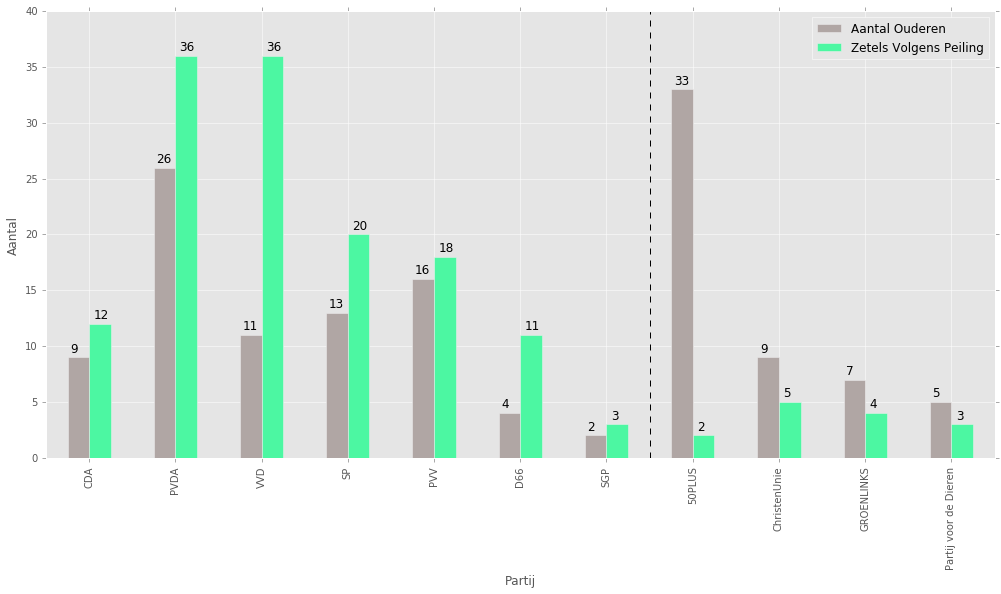
\includegraphics[width=0.98\linewidth]	{Aantal_ouderen_aantal_zetels1.png}

			\caption{Het aantal ouderen op de kandidatenlijst(grijs) en het aantal zetels volgens de peilingen(groen) per partij.}

\label{fig:zetelsO}
\end{figure}

\paragraph{Maximaal aantal ouderen per partij (top \textit{N}) dat in de Tweede Kamer gekozen kan worden.}
In Tabel \ref{table:tab3O} hieronder is, in het verlengde van Figuur \ref{fig:zetelsO} hierboven, te zien hoeveel oudere kandidaten er per partij maximaal in de Tweede Kamer gekozen hadden kunnen worden. In de Tabel is dus per partij het aantal (\textit{N}) oudere kandidaten te zien waarover de stemmen van de oudere kiezers op de partij verdeeld zullen worden.  

Vanwege het feit dat het CDA, D66, de PVDA, de PVV, de SGP, de SP en de VVD volgens de peiling \cite{IPSOS} meer zetels zouden gaan ontvangen dan zij ouderen op de kandidatenlijst hadden staan, komt het totaal aantal oudere kandidaten dat volgens de peiling in de Tweede Kamer gestemd had kunnen worden op 95.




\begin{table}[h]
\centering
	\begin{footnotesize}
		\begin{tabular}{lrr}
\toprule
{} &  Top \textit{N} Oudere Kandidaten &  Overgebleven Kandidaten \\
Partij                &                          &                          \\
\midrule
50PLUS                &                        2 &                        0 \\
CDA                   &                        9 &                        3 \\
ChristenUnie          &                        5 &                        0 \\
D66                   &                        4 &                        7 \\
GROENLINKS            &                        4 &                        0 \\
Partij v d Dieren &                        3 &                        0 \\
PVDA                  &                       26 &                       10 \\
PVV                   &                       16 &                        2 \\
SGP                   &                        2 &                        1 \\
SP                    &                       13 &                        7 \\
VVD                   &                       11 &                       25 \\
\midrule
Toaal				  & 						95&                        55\\
\bottomrule
\end{tabular}

	\end{footnotesize}
			\caption{Per partij de top \textit{N} oudere kandidaten en de overgebleven kandidaten met een leeftijd van onder de 50 jaar a.d.h.v. de peiling.}
\label{table:tab3O} 
\end{table}



\paragraph{Het toewijzen van de stemmen aan de oudere kandidaten op basis van de peiling en de einduitslag.}
Op dezelfde wijze als bij de andere strategie\"{e}n wijzen we de hier de oudere stemmen toe a.d.h.v. de peiling en a.d.h.v. de einduitslag (voor gedetailleerde uitleg zie \hyperref[S1V]{Strategie 1} in \hyperref[vrouwen]{Bevolkingsgroep: Vrouwen}). In Figuur \ref{fig:stemmenS1O} hieronder is zowel de toewijzing op basis van de peiling alsmede de toewijzing op basis van de einduitslag te zien.


\begin{figure}[H]

	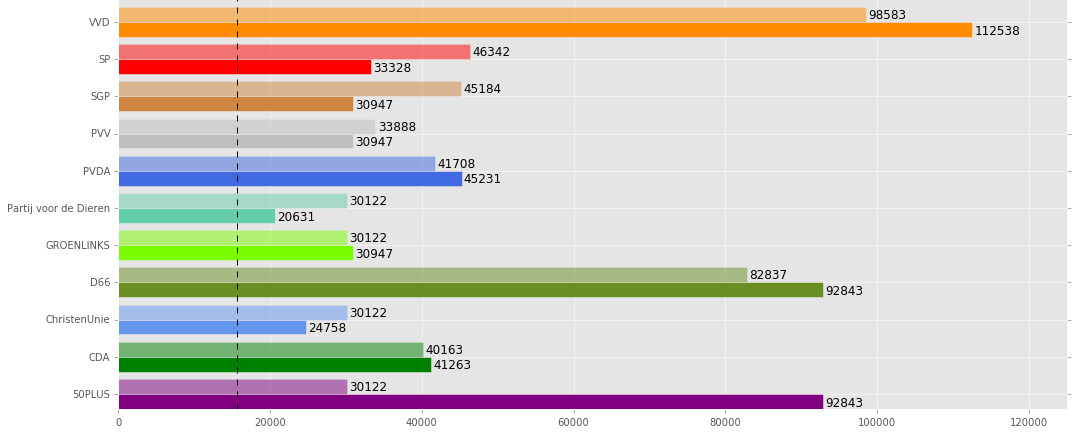
\includegraphics[width=\linewidth]	{stemmen_op_ouderen_topN_peiling.png}

			\caption{Grafiek met per partij de verdeling van de stemmen van oudere kiezers op de top \textit{N} oudere kandidaten van de partij a.d.h.v. de peiling \citep{IPSOS} in de licht gekleurd staven en a.d.h.v. de einduitslag \citep{Kiesraad_databank} in de donker gekleurde staven. De stippellijn is de daadwerkelijk voorkeursdrempel(15.708 stemmen).}

\label{fig:stemmenS1O}
\end{figure}


Zoals te zien in Figuur \ref{fig:stemmenS1O} hierboven, zouden zowel volgens de peiling (voorspelling) alsmede volgens de einduitslag alle top \textit{N} oudere kandidaten van de partijen boven de daadwerkelijke voorkeursdrempel uitgekomen zijn. Ofschoon de precieze aantallen niet exact hetzelfde zijn, is met strategie 2 de voorspelling zoals berekend a.d.h.v. de peiling correct in het voorspellen welke partijen met alle oudere kandidaten boven de voorkeursdrempel uitgekomen zouden zijn en bij welke partijen dit niet het geval zou zijn geweest.

\paragraph{Aantal ouderen na strategie 1.}
Na het uitvoeren van de strategie 1 en het opstellen van de Tweede Kamer zoals eerder in dit hoofdstuk beschreven, zou strategie 1 een Tweede Kamer hebben opgeleverd op waarin  89 ouderen en 61 personen van onder de vijftig jaar zouden hebben plaatsgenomen. Daarmee zouden ouderen (met 59\%) ruim in betere mate vertegenwoordigd zijn geweest dan personen van onder de 50 jaar (met 41\%). In de cirkeldiagram in Figuur \ref{fig:pcS1O} hieronder is de verdeling goed te zien. 

\begin{figure}[H]
\centering
	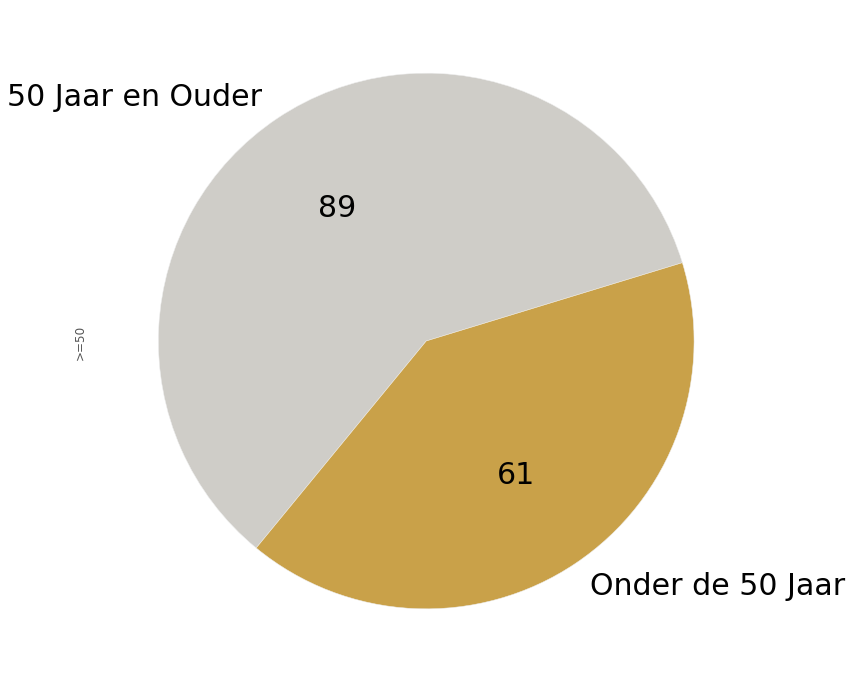
\includegraphics[width=0.42\linewidth]{pie_chart_topN_ouderen.png}

			\caption{Na uitvoering van de strategie nemen er 89 ouderen(59\%) en 61 personen onder de 50 (41\%) plaats in de Tweede Kamer.}

\label{fig:pcS1O}
\end{figure}

\paragraph{Minder dan 95 ouderen in de Tweede Kamer na uitvoering van strategie 1.}
De reden dat er niet 95 ouderen maar 'slechts' 89 ouderen in de Tweede Kamer zouden hebben plaatsgenomen na uitvoering van strategie 1 ligt ten grondslag aan een aantal factoren. Bij GROENLINKS had de lijsttrekker, in de persoon van Jolande 
Sap, meer stemmen dan de oudere kandidaten. Hierdoor zou bij GROENLINKS één oudere kandidaat afgevallen zijn. De Partij voor de Dieren had de lijsttrekker, in de persoon van Marianne Thieme, ook meer stemmen dan de oudere kandidaten. Tevens ontving de Partij voor de Dieren één zetel minder bij de einduitslag dan dat de peiling aangaf. Hierdoor zouden er bij de Partij voor de Dieren twee oudere kandidaten afgevallen zijn. Bij de PVV hadden zowel de lijsttrekker (Geert Wilders) als de nummer twee op de lijst (Fleur Agema) meer stemmen dan de oudere kandidaten gehad zouden hebben. Tevens ontving de PVV drie zetels minder bij de einduitslag dan dat de peiling aangaf. Hierdoor zouden er bij de PVV drie oudere kandidaten afgevallen zijn. Het aantal ouderen in de Tweede Kamer na uitvoering van strategie 1 komt daarom uit op ($95-6$ = ) 89. 




\subsubsection{Strategie 2: Oudere kiezers stemmen op een willekeurige oudere kandidaat.}

\paragraph{Het toewijzen van de stemmen aan de oudere kandidaten op basis van de peiling en de einduitslag.}
Op dezelfde wijze als bij de andere strategie\"{e}n wijzen we de hier de oudere stemmen toe a.d.h.v. de peiling en a.d.h.v. de einduitslag (voor gedetailleerde uitleg zie \hyperref[S1V]{Strategie 1} in \hyperref[vrouwen]{Bevolkingsgroep: Vrouwen}). In Figuur \ref{fig:stemmenS2O} hieronder is zowel de toewijzing op basis van de peiling alsmede de toewijzing op basis van de einduitslag te zien.
Zoals te zien in Figuur \ref{fig:stemmenS2O} hieronder, zouden zowel volgens de peiling (voorspelling) alsmede volgens de einduitslag niet alle oudere kandidaten van de partijen boven de daadwerkelijke voorkeursdrempel uitgekomen zijn. Ofschoon de precieze aantallen niet exact hetzelfde zijn, is met strategie 2 de voorspelling zoals berekend a.d.h.v. de peiling grotendeels correct in het voorspellen welke partijen met alle oudere kandidaten boven de voorkeursdrempel uitgekomen zouden en welke partijen dit niet het geval zou zijn geweest. Enkel bij de Partij voor de Dieren en bij de ChristenUnie is er voorspeld dat de oudere kandidaten aan de voorkeursdrempel zou voldoen terwijl niet bij de einduitslag niet het geval geweest zou zijn.

\begin{figure}[H]

	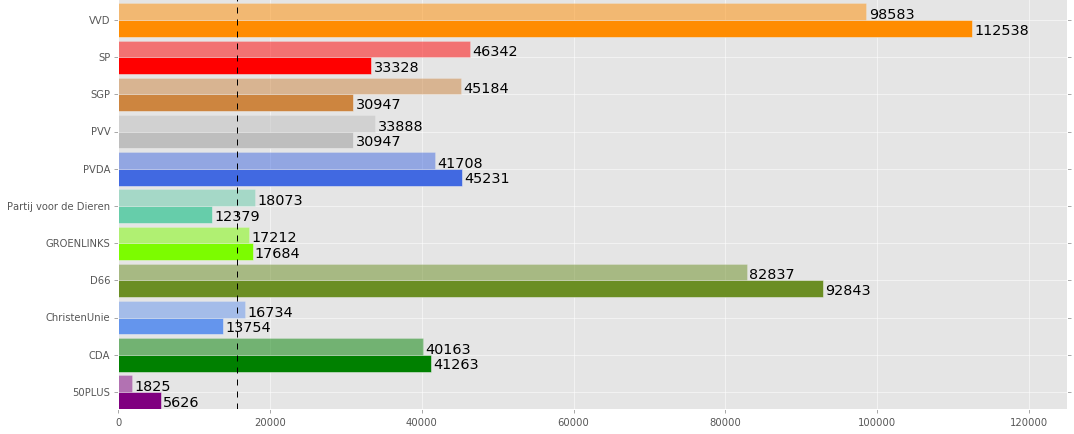
\includegraphics[width=\linewidth]	{stemmen_op_ouderen_willekeurig_samen.png}

			\caption{Grafiek met per partij de verdeling van de stemmen van oudere kiezers op alle oudere kandidaten van de partij a.d.h.v. de peiling \citep{IPSOS} in de licht gekleurd staven en a.d.h.v. de einduitslag \citep{Kiesraad_databank} in de donker gekleurde staven. De stippellijn is de daadwerkelijk voorkeursdrempel(15.708 stemmen).}

\label{fig:stemmenS2O}
\end{figure}

Zoals te zien in Figuur \ref{fig:stemmenS2O} hierboven, zouden zowel volgens de peiling (voorspelling) alsmede volgens de einduitslag niet alle oudere kandidaten van de partijen boven de daadwerkelijke voorkeursdrempel uitgekomen zijn. Ofschoon de precieze aantallen niet exact hetzelfde zijn, is met strategie 2 de voorspelling zoals berekend a.d.h.v. de peiling grotendeels correct in het voorspellen welke partijen met alle oudere kandidaten boven de voorkeursdrempel uitgekomen zouden en welke partijen dit niet het geval zou zijn geweest. Enkel bij de Partij voor de Dieren en bij de ChristenUnie is er voorspeld dat de oudere kandidaten aan de voorkeursdrempel zou voldoen terwijl niet bij de einduitslag niet het geval geweest zou zijn.

\paragraph{Aantal ouderen na strategie 2.}
Na het uitvoeren van de strategie 2 en het opstellen van de Tweede Kamer zoals eerder in dit hoofdstuk beschreven, zou strategie 2 een Tweede Kamer hebben opgeleverd op waarin 84 ouderen en 66 personen onder de vijftig jaar zouden hebben plaatsgenomen. Daarmee zouden ouderen (met 56\%) ruim in betere mate vertegenwoordigd zijn geweest dan personen van onder de vijftig jaar (met 44\%). In de cirkeldiagram in Figuur \ref{fig:pcS2O} hieronder is de verdeling goed te zien. 


\begin{figure}[H]
\centering
	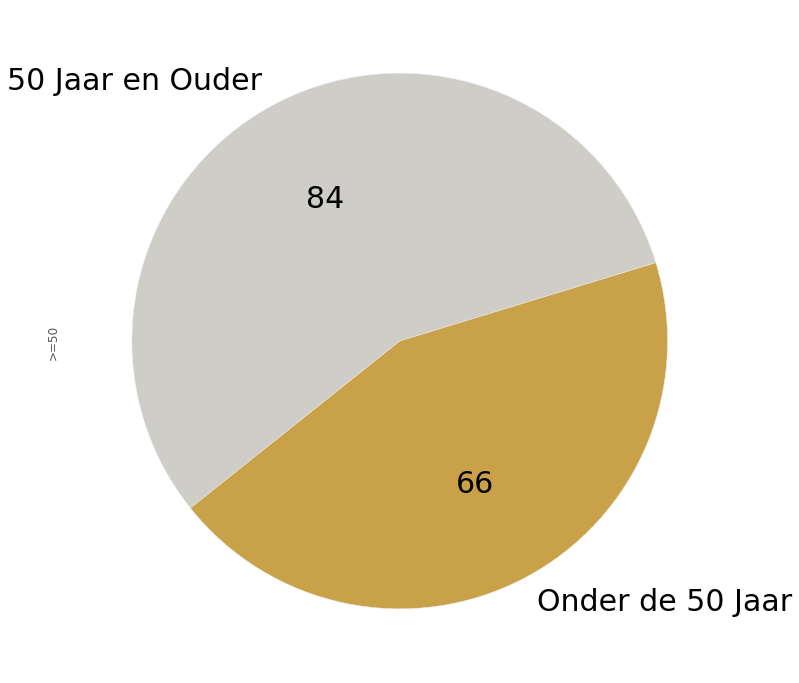
\includegraphics[width=0.42\linewidth]{pie_chart_willekeurig_ouderen.png}

			\caption{Na uitvoering van de strategie nemen er 84 ouderen(56\%) en 66 personen onder de 50(44\%) plaats in de Tweede Kamer.}

\label{fig:pcS2O}
\end{figure}





\paragraph{Één oudere minder in de Tweede Kamer ten opzicht van strategie 1.}
De reden dat er niet 89 maar 84 ouderen in de Tweede Kamer zouden hebben plaatsgenomen na uitvoering van strategie 2 ligt ten grondslag aan een aantal factoren. Bij de Partij voor de Dieren en bij de ChristenUnie zouden de oudere kandidaten niet genoeg stemmen hebben ontvangen aan de voorkeursdrempel te voldoen. Hierdoor zouden er bij deze partijen in totaal vijf oudere kandidaten afgevallen zijn. Hoewel ook bij 50PLUS de oudere kandidaten ook te weinig stemmen zouden hebben gekregen om aan de voorkeursdrempel te voldoen, had 50PLUS enkel ouderen op de kandidatenlijst staan. Hierdoor zouden er bij 50PLUS geen oudere kandidaten zijn afgevallen. 




%\titlespacing*{\subsubsection}{0pt}{30pt}{10pt}
\subsubsection{Strategie 3.1: Oudere kiezers stemmen willekeurige op één van de eerste 15 oudere kandidaten van een partij.}

\paragraph{Partijen met minstens 15 oudere kandidaten en partijen met minder dan 15 oudere kandidaten.}
In de grafiek in Figuur \ref{fig:15O} hieronder zien we dat bij 50PLUS, de PVDA en de PVV de stemmen van oudere kiezers over de top 15 oudere kandidaten verdeeld hadden kunnen worden. Bij de overige partijen hadden de stemmen van oudere kiezers die de partij volgens de peiling zou gaan ontvangen verdeeld moeten worden over alle oudere kandidaten die deze partijen op hun kandidatenlijsten hadden staan.




\begin{figure}[H]

	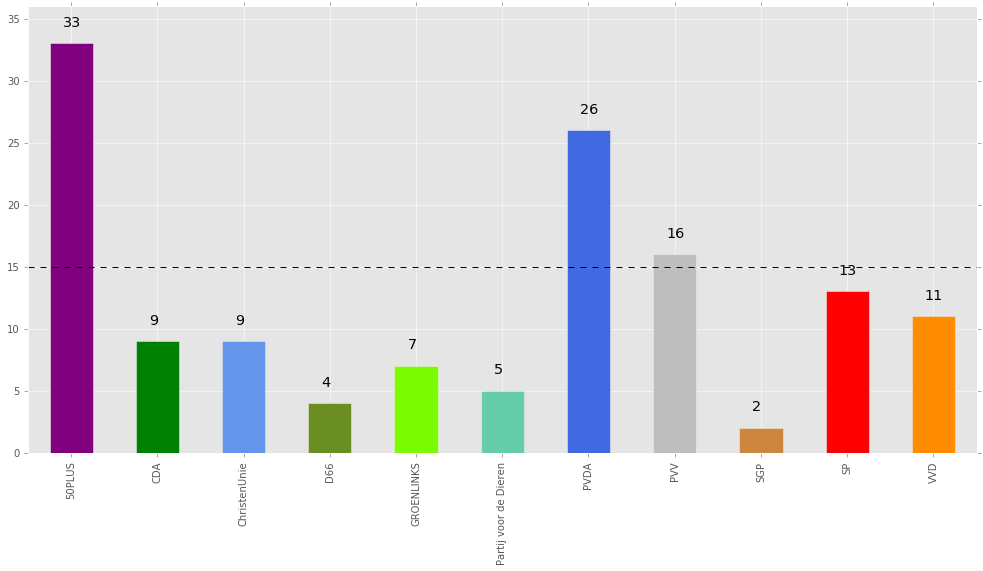
\includegraphics[width=\linewidth]	{top15_of_topN_kandidaten_ouderen.png}

			\caption{De grafiek toont bij welke partijen de oudere kiezers op de top 15 oudere kandidaten van de partij kunnen gaan stemmen (\textit{N=15}) en van welke partijen de oudere kiezers op alle oudere kandidaten van de partij kunnen gaan stemmen (\textit{N=totaal aantal oudere kandidaten}).} 


\label{fig:15O}
\end{figure}



\paragraph{Het toewijzen van de stemmen aan de oudere kandidaten op basis van de peiling en de einduitslag.}
Op dezelfde wijze als bij de andere strategie\"{e}n wijzen we de hier de oudere stemmen toe a.d.h.v. de peiling en a.d.h.v. de einduitslag (voor gedetailleerde uitleg zie \hyperref[S1V]{Strategie 1} in \hyperref[vrouwen]{Bevolkingsgroep: Vrouwen}). In Figuur \ref{fig:stemmenS31O} hieronder is zowel de toewijzing op basis van de peiling alsmede de toewijzing op basis van de einduitslag te zien.

\begin{figure}[H]

	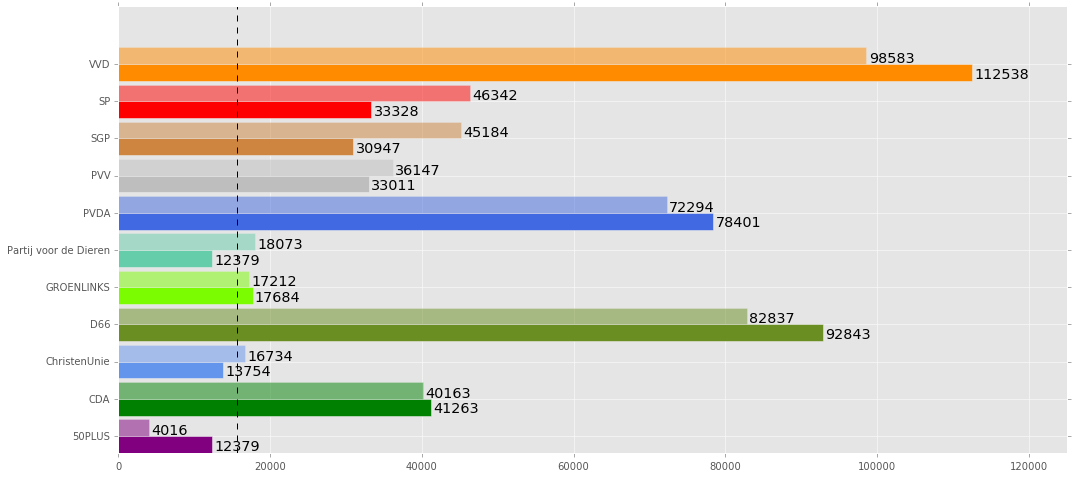
\includegraphics[width=\linewidth]	{stemmen_op_ouderen_top15_of_topN_samen.png}

			\caption{Grafiek met per partij de verdeling van de stemmen van oudere kiezers op alle oudere kandidaten van de partij a.d.h.v. de peiling \citep{IPSOS} in de licht gekleurd staven en a.d.h.v. de einduitslag \citep{Kiesraad_databank} in de donker gekleurde staven. De stippellijn is de daadwerkelijk voorkeursdrempel(15.708 stemmen).}

\label{fig:stemmenS31O}
\end{figure}

Zoals te zien in Figuur \ref{fig:stemmenS31O} hierboven, zouden zowel volgens de peiling (voorspelling) alsmede volgens de einduitslag niet alle oudere kandidaten van de partijen boven de daadwerkelijke voorkeursdrempel uitgekomen zijn. Ofschoon de precieze aantallen niet exact hetzelfde zijn, is met strategie 3.1 de voorspelling zoals berekend a.d.h.v. de peiling grotendeels correct in het voorspellen welke partijen welke partijen met de top \textit{N} (\textit{N=15} of \textit{N=totaal aantal oudere kandidaten}) oudere kandidaten aan de voorkeursdrempel voldoen en bij welke partijen dit niet het geval zou zijn geweest. Enkel bij de Partij voor de Dieren en bij de ChristenUnie is er voorspeld dat de top \textit{N} oudere kandidaten boven de voorkeursdrempel uit zouden komen terwijl niet bij de einduitslag niet zo zou zijn.

\paragraph{Aantal ouderen na strategie 3.1.}
Na het uitvoeren van de strategie 3.1 en het opstellen van de Tweede Kamer zoals eerder in dit hoofdstuk beschreven, zou strategie 3.1 uiteindelijk een Tweede Kamer hebben opgeleverd waarin 73 ouderen en 77 personen onder vijftig jaar plaatsnemen. Daarmee zouden ouderen(met 49\%) net aan in mindere mate vertegenwoordigd zijn geweest dan personen van onder de vijftig jaar jaar(met 51\%). In de cirkeldiagram in Figuur \ref{fig:pcS31O} hieronder is de verdeling goed te zien. In de volgende paragraaf wordt uitgelegd waarom er niet 84 (zoals in de vorige strategie) maar slechts 73 ouderen in de Tweede Kamer zouden hebben plaatsgenomen na uitvoering van strategie 3.1 ten opzichte van strategie 2.

\begin{figure}[H]
\centering
	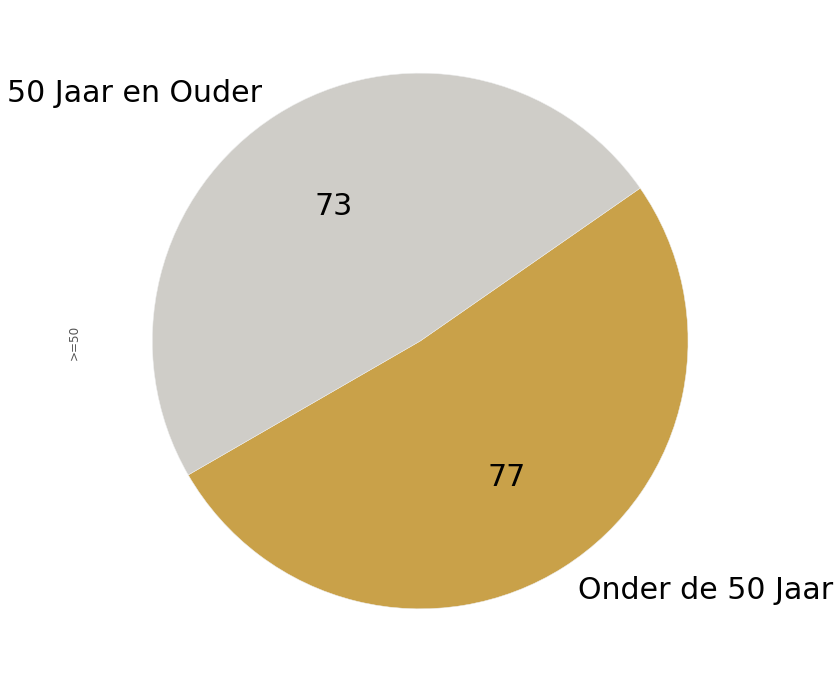
\includegraphics[width=0.42\linewidth]{pie_chart_top15_of_topN_ouderen.png}

			\caption{Na uitvoering van de strategie nemen er 73 ouderen (49\%) en 77 personen onder de 50 jaar (51\%) plaats in de Tweede Kamer.}

\label{fig:pcS31O}
\end{figure}

\paragraph{Minder vrouwen in de Tweede Kamer d.m.v. uitvoering van strategie 3.1 dan d.m.v. uitvoering van strategie 2.}
De reden dat er, na uitvoering van strategie 3.1, 73 ouderen in de Tweede Kamer zouden hebben plaatsgenomen en dat er daarmee elf ouderen minder zouden hebben plaatsgenomen in de Tweede Kamer dan bij strategie 2 het geval zou zijn geweest, ligt ten grondslag aan het feit dat er bij de PVDA elf oudere kandidaten zouden zijn afgevallen ten opzichte van strategie 2. Dit komt omdat de stemmen niet verdeeld zouden zijn over alle 26 oudere kandidaten van de PVDA maar over de top 15 oudere kandidaten van de PVDA. De overige elf oudere kandidaten van de PVDA stonden niet hoog genoeg op de kandidatenlijst om een zetel te hebben ontvangen. Daarmee zou het totale aantal ouderen in de Tweede Kamer uitgekomen zijn ($84-11$ = ) 73.






\subsubsection{Strategie 3.2: Oudere kiezers stemmen willekeurige op één van de eerste \textit{N} oudere kandidaten van een partij.}


\paragraph{Voor elke partij de eigen \textit{N} bepalen.}
Hieronder is in de grafiek in Figuur \ref{fig:XO} per partij te zien op welke waarde het \textit{N} oudere kandidaten wordt bepaald. Het CDA, de ChristenUnie, GROENLINKS en de Partij voor de Dieren hadden allemaal minder dan tien oudere kandidaten op de kandidatenlijst staan en daardoor geldt voor deze partijen \textit{N=5}. Ook de SGP en D66 hadden minder dan tien oudere kandidaten op de kandidatenlijst. Deze partijen hebben echter zelfs minder dan vijf oudere kandidaten op de kandidatenlijst staan. Hierdoor geld voor deze partijen een \textit{N=totaal aantal oudere kandidaten}. Voor de SGP geldt $N=2$ en voor D66 geldt $N=4$. De SP en de VVD hadden tien of meer oudere kandidaten op de kandidatenlijsten maar minder dan vijftien. Hierdoor geldt voor deze partijen $N=10$. De PVDA en de PVV hadden vijftien of meer oudere kandidaten op de kandidatenlijsten maar minder dan dertig. Hierdoor geldt voor deze partijen $N=30$. Enkel de 50PLUS had meer dan dertig oudere kandidaten op de kandidatenlijst staan en daardoor geldt voor 50PLUS $N=30$. 

\begin{figure}[H]

	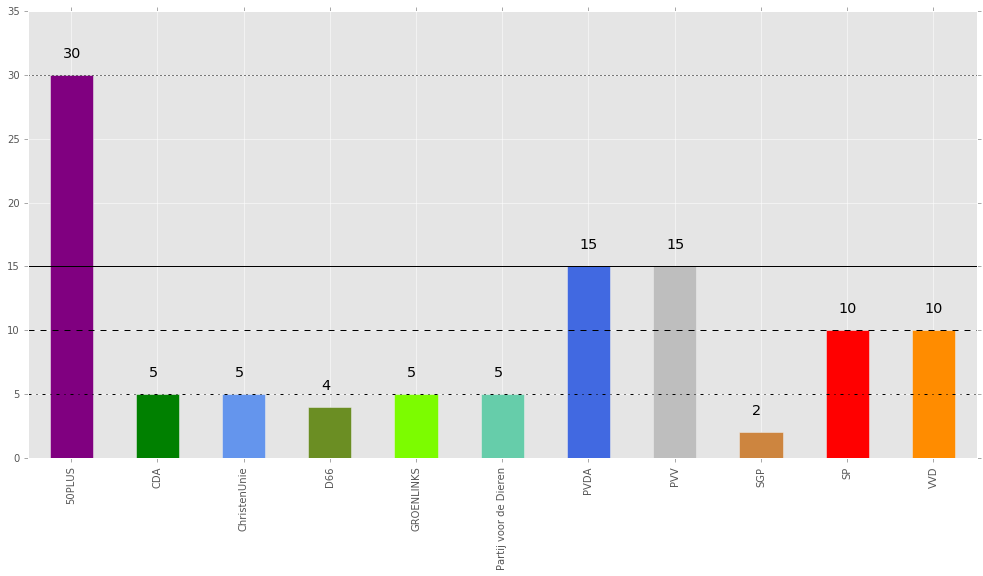
\includegraphics[width=\linewidth]{eigenX_partijen_ouderen.png}
		\caption{Elke partij krijgt een eigen \textit{N}. De lijnen geven een mogelijke \textit{N} aan.}

\label{fig:XO}
\end{figure}





\paragraph{Het toewijzen van de stemmen aan de oudere kandidaten op basis van de peiling en de einduitslag.}
Op dezelfde wijze als bij de andere strategie\"{e}n wijzen we de hier de oudere stemmen toe a.d.h.v. de peiling en a.d.h.v. de einduitslag (voor gedetailleerde uitleg zie \hyperref[S1V]{Strategie 1} in \hyperref[vrouwen]{Bevolkingsgroep: Vrouwen}). In Figuur \ref{fig:stemmenS32O} hieronder is zowel de toewijzing op basis van de peiling alsmede de toewijzing op basis van de einduitslag te zien.


\begin{figure}[H]

	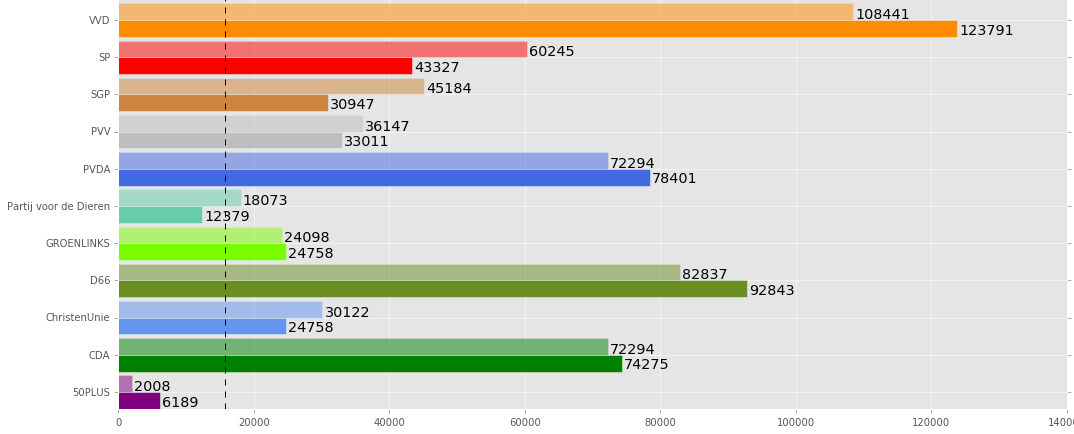
\includegraphics[width=\linewidth]{stemmen_op_ouderen_eigenX_samen.png}

			\caption{Grafiek met per partij de verdeling van de stemmen van oudere kiezers op alle oudere kandidaten van de partij a.d.h.v. de peiling \citep{IPSOS} in de licht gekleurd staven en a.d.h.v. de einduitslag \citep{Kiesraad_databank} in de donker gekleurde staven. De stippellijn is de daadwerkelijk voorkeursdrempel(15.708 stemmen).}

\label{fig:stemmenS32O}
\end{figure}

Zoals te zien in Figuur \ref{fig:stemmenS32O} hierboven, zouden zowel volgens de peiling (voorspelling) alsmede volgens de einduitslag niet alle oudere kandidaten van de partijen aan de daadwerkelijke voorkeursdrempel hebben voldaan. Ofschoon de precieze aantallen niet exact hetzelfde zijn, is met strategie 3.2 de voorspelling zoals berekend a.d.h.v. de peiling grotendeels correct in het voorspellen welke partijen welke partijen met de top \textit{N} ($N=5$, $N=10$, $N=15$, $N=30$ of $N=$totaal aantal oudere kandidaten) oudere kandidaten aan de voorkeursdrempel zouden hebben voldaan en welke partijen dit niet het geval zou zijn geweest. Enkel is ook bij strategie 3.2 voor de Partij voor de Dieren voorspeld dat de top \textit{N} oudere kandidaten (voor de Partij voor de Dieren geldt $N=5$) boven de voorkeursdrempel uit zouden komen terwijl niet bij de einduitslag niet het geval zou zijn geweest. Dit ligt ten grondslag aan het feit dat de Partij voor de Dieren een kleiner aantal stemmen kreeg dan de peiling had voorspeld. 


\paragraph{Aantal ouderen na strategie 3.2.}
Na het uitvoeren van de strategie 3.2 en het opstellen van de Tweede Kamer zoals eerder in dit hoofdstuk beschreven, zou strategie 3.2 een Tweede Kamer hebben opgeleverd waarin 69 ouderen en 81 personen onder de vijftig jaar zouden hebben plaatsgenomen. Daarmee zouden ouderen (met 46\%) in mindere mate vertegenwoordigd zijn geweest dan personen onder de vijftig jaar (met 54\%). In de cirkeldiagram in Figuur \ref{fig:pcS32O} hieronder is de verdeling goed te zien. In de volgende paragraaf wordt uitgelegd waarom er acht ouderen minder in de Tweede Kamer zouden hebben plaatsgenomen na uitvoering van strategie 3.2 ten opzicht van strategie 3.1.

\begin{figure}[H]
\centering
	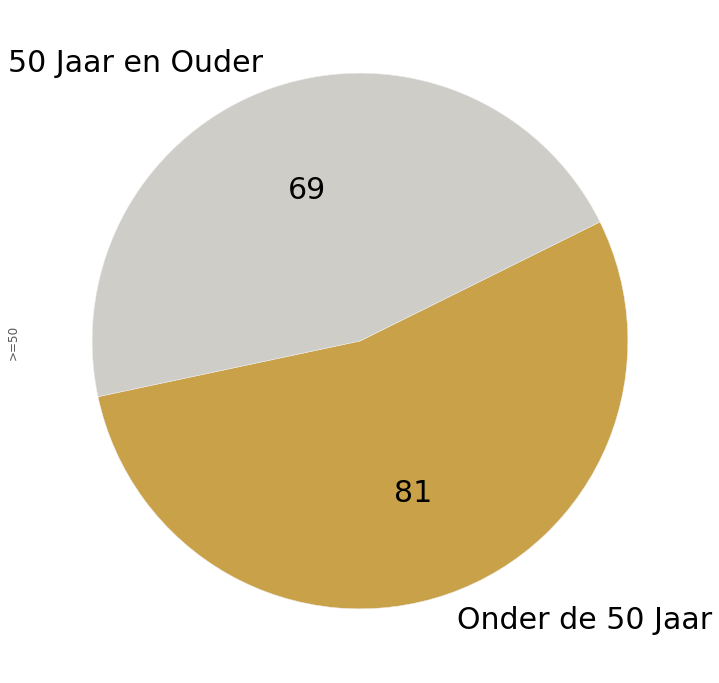
\includegraphics[width=0.40\linewidth]{pie_chart_eigenX_ouderen.png}

\caption{Na uitvoering van de strategie nemen er 69 ouderen(58.7\%) en 81 personen onder de 50(41.3\%) plaats in de Tweede Kamer.} 

\label{fig:pcS32O}
\end{figure}

\paragraph{Meer ouderen in de Tweede Kamer d.m.v. uitvoering van strategie 3.2 dan d.m.v. uitvoering van strategie 3.1.}
De reden dat er, na uitvoering van strategie 3.2, 69 ouderen in de Tweede Kamer plaatsnemen en dat er daarmee vier ouderen minder zouden zijn geweest ten opzichte van strategie 3.1 ligt ten grondslag aan het feit dat bij het CDA vier oudere kandidaten zouden zijn afgevallen. Het CDA had negen oudere kandidaten op de kandidatenlijst. Door uitvoering van strategie 3.2 zouden de oudere stemmen op het CDA echter verdeeld zijn geweest over de top vijf oudere kandidaten van het CDA. Op dezelfde manier zouden er bij de SP drie oudere kandidaten afgevallen zijn (dertien oudere kandidaten op de kandidatenlijst, tien oudere kandidaten waarover de oudere stemmen verdeeld zouden zijn geweest) en bij de VVD zou er één oudere kandidaat af zijn gevallen (elf oudere kandidaten op de kandidatenlijst, tien oudere kandidaten waarover de oudere stemmen verdeeld zouden zijn geweest). De oudere top 5 oudere kandidaten van de ChristenUnie zouden met strategie 3.2 echter wel boven de kiesdrempel uit zijn gekomen. Hierdoor komen er vier ouderen voor de ChristenUnie in de Tweede Kamer bij. Daarmee komt het totale aantal ouderen in de Tweede Kamer uit op ($73-4$ = )69.








\subsubsection{Strategie 4: Ouderen kiezers stemmen op de top \textit{N+extra percentage} oudere kandidaten van een partij.}

\paragraph{Speling in top \textit{N}.}
Zoals te zien in Figuur \ref{fig:zetelsO}, zijn er meerdere partijen die een hoger aantal oudere kandidaten op de kandidatenlijst hadden staan dan dat verwacht werd dat zij, volgens de peiling, aan zetels zouden gaan ontvangen. Vanwege het feit dat de zetelverdeling volgens de peiling niet 100\% correspondeerde met de zetelverdeling volgens de einduitslag, is het ook voor de bevolkingsgroep ouderen interessant om te kijken wat er zou zijn gebeurd wanneer de top \textit{N} wordt uitgebreid met een \textit{extra percentage} bovenop de eerder al per partij bepaalde top \textit{N} uit strategie 1.



\paragraph{Maximaal aantal ouderen per partij(top \textit{N+extra percentage}) dat in de Tweede Kamer gekozen had kunnen worden.} 
Bij strategie 4 wordt de top \textit{N} voor elke partij uitgebreid met een \textit{extra percentage} van \textit{N} in stappen van 10\% extra (dus eerst 110\%, dan 120\% etc.). Zodoende worden de oudere stemmen die een partij ontvangt telkens over de top \textit{N+extra percentage} oudere kandidaten van de partij verdeeld. Daarbij kan de top \textit{N+extra percentage} van een partij nooit meer worden dat het totaal aantal oudere kandidaten dat de partij op de kandidatenlijst heeft staan. In Figuur \ref{fig:NexpO} hieronder is er per partij te zien wat er met de top \textit{N} gebeurt wanneer het \textit{extra percentage} hieraan wordt toegevoegd.  


\begin{figure}[H]

	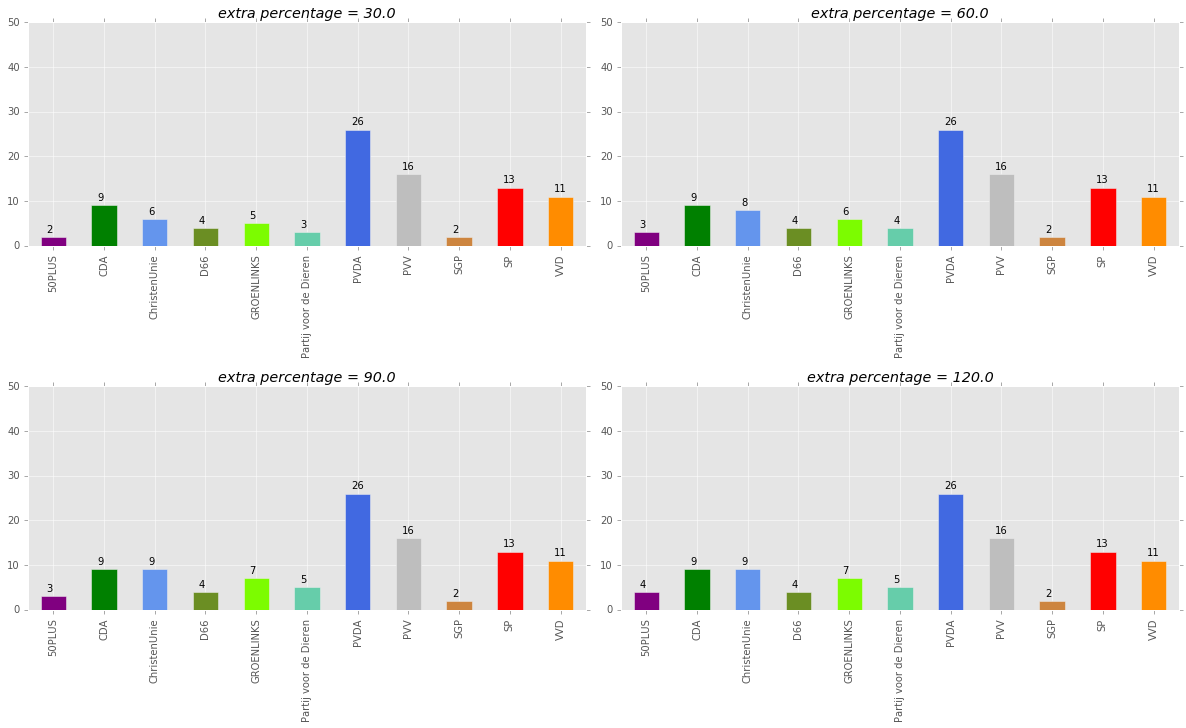
\includegraphics[width=\linewidth]{topN_vermenigvuldiging_ouderen.png}

			\caption{De top \textit{N+extra percentage} waarin \textit{extra percentage} respectievelijk 30\%, 60\%, 90\% en 120\% extra te verwachten zetels (voor oudere kandidaten)  zijn.}

\label{fig:NexpO}
\end{figure}



\paragraph{Het toewijzen van de stemmen aan de oudere kandidaten op basis van de peiling en de einduitslag.}
Op dezelfde wijze als bij de andere strategie\"{e}n wijzen we de hier de oudere stemmen toe a.d.h.v. de peiling en a.d.h.v. de einduitslag (voor gedetailleerde uitleg zie \hyperref[S1V]{Strategie 1} in \hyperref[vrouwen]{Bevolkingsgroep: Vrouwen}). In de grafieken in Figuur \ref{fig:stemmenS4O} hieronder is zowel de toewijzing van oudere stemmen op oudere kandidaten op basis van de peiling alsmede op basis van de einduitslag voor alle partijen te zien. De toewijzingen worden getoond aan de hand van respectievelijk 30\%, 60\%, 90\% en 120\% (\textit{extra percentage}) extra zetels (voor oudere kandidaten) waarover de stemmen verdeeld worden.

In Figuur \ref{fig:stemmenS4O} hierboven, is te zien dat zowel volgens de peiling (voorspelling) alsmede volgens de einduitslag niet alle top \textit{N+extra percentage} oudere kandidaten van de partijen boven de daadwerkelijke voorkeursdrempel uitgekomen zouden zijn wanneer het \textit{extra percentage} aan zetels (voor oudere kandidaten) wordt verhoogd. Echter gebeurt dit pas tussen de 30\%  en 60\% extra zetels (voor oudere kandidaten) waarover de stemmen verdeeld worden. Ofschoon de precieze aantallen niet exact hetzelfde zijn, is met strategie 4 de voorspelling zoals berekend a.d.h.v. de peiling grotendeels correct in het voorspellen welke partijen met de top \textit{N+extra percentage} oudere kandidaten boven de voorkeursdrempel uitgekomen zouden zijn en van welke partijen dit niet het geval zou zijn geweest.
  
\begin{figure}[H]

	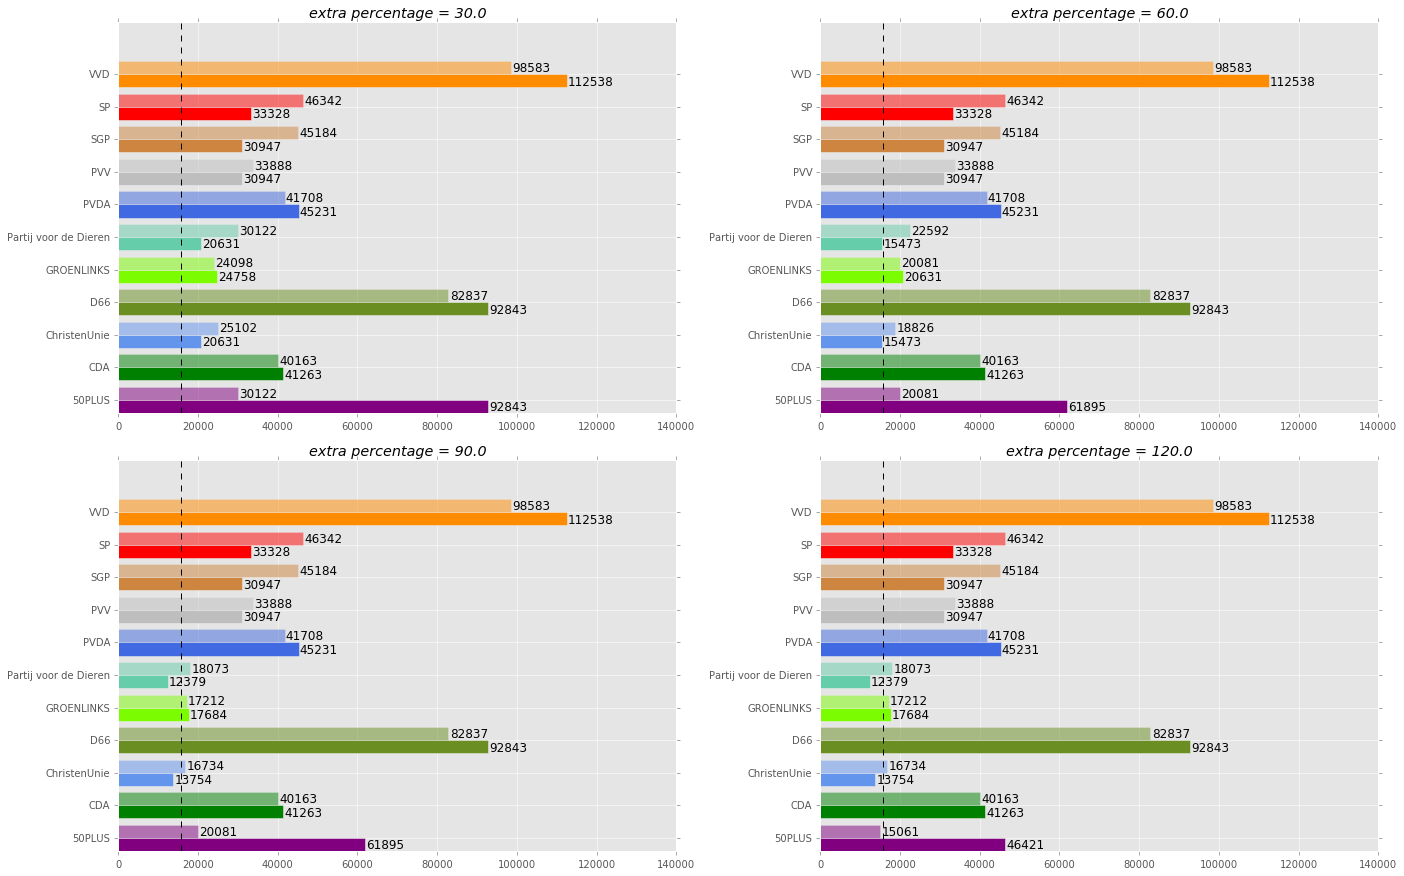
\includegraphics[width=\linewidth]	{stemmen_op_ouderen_topNextrapercentage_samen.png}

			\caption{Grafieken in stappen van 30\%, met per partij de verdeling van de stemmen van oudere kiezers op de top \textit{N+extra percentage} oudere kandidaten van de partij a.d.h.v. de peiling (licht gekleurd) en a.d.h.v. de einduitslag (donker gekleurd). De stippellijn is de daadwerkelijk voorkeursdrempel(15.708 stemmen).} 

\label{fig:stemmenS4O}
\end{figure}





\paragraph{Aantal ouderen na strategie 4.}
Na het uitvoeren van strategie 4 en het opstellen van de Tweede Kamer zoals eerder in dit hoofdstuk beschreven, zou strategie 4 bij geen enkel \textit{extra percentage} bovenop de originele \textit{N} uit strategie 1 een hoger aantal ouderen in de Tweede Kamer hebben opgeleverd. In de grafiek hieronder in Figuur \ref{fig:bcS4O} is te zien hoeveel ouderen er in de Tweede Kamer een zetels bedeeld zouden hebben gekregen wanneer er een bepaald \textit{extra percentage} wordt toegevoegd aan de originele \textit{N} uit strategie 1.



\begin{figure}[H]

	\includegraphics[width=\linewidth]	{topNextrapercentage_aantal_ouderen_overzicht.png}

			\caption{Grafiek met per het aantal ouderen in de Tweede Kamer na uitvoering(en) van strategie 4 in stappen van 10\% aan \textit{extra percentage} (van \textit{N}) bovenop de \textit{N} uit strategie 1. }

\label{fig:bcS4O}
\end{figure}

\paragraph{Niet meer maar minder ouderen na uitvoering van strategie 4.}
Zoals hierboven in Figuur \ref{fig:bcS4O} te zien, komen er na uitvoering van strategie 4 en het toenemen van het \textit{extra percentage} op geen enkel moment meer ouderen in de Tweede Kamer dan de 121 uit strategie 1 (0\% staat in de grafiek gelijk aan strategie 1.) 


\paragraph{Niet meer dan 89 ouderen in de Tweede Kamer.}
De reden dat er niet meer dan 89 ouderen in de Tweede Kamer plaatsnemen na uitvoering van strategie 4 ligt ten grondslag aan een aantal factoren. Willen er meer ouderen in de Tweede Kamer plaatsnemen dan na uitvoering van strategie 1 dan is het noodzakelijk dat de partijen ook meer zetels kregen bedeeld bij de einduitslag dan dat volgens te peiling was te verwachten. 

Zo hadden de meeste partijen een kleiner aantal (of een gelijk aantal) ouderen op de kandidatenlijst staan als dat de peiling aangaf dat zij aan zetels zouden gaan ontvangen. Hierdoor zou de top \textit{N} van deze partijen niet zijn uitgebreid wanneer het \textit{extra percentage} aan de \textit{N} werd toegevoegd. De Partij voor de Dieren, 50PLUS, de ChristenUnie en GROENLINKS kregen bij de einduitslag niet meer zetels dan volgens de peiling werd verwacht. Zodoende had het aantal ouderen die in de Tweede Kamer zou hebben plaatsgenomen nooit op meer dan 89 uit zijn gekomen.


\subsection{Bevolkingsgroep: Provincialen.} \label{provincialen}
Betreffende de bevolkingsgroep provincialen in Nederland worden hieronder de resultaten van de verschillende strategie\"{e}n uiteengezet om zodoende te achterhalen met welke strategie in theorie de meeste provinciale kandidaten in de Tweede Kamer gekozen hadden kunnen worden wanneer alle stemgerechtigde provincialen kiezers in Nederland zich hadden gecommitteerd aan de strategie bij de Tweede Kamerverkiezingen van 2012.\\
\indent Ten behoeve van de leesbaarheid worden er geen voorbeelden gegeven betreffende berekeningen. Alle voorbeelden zijn te vertalen vanuit de bij de bevolkingsgroep vrouwen toegepaste strategie\"{e}n (zie Sectie \ref{vrouwen}). 

\paragraph{Aannames en Regels.}
De aannames en regels zijn hetzelfde als bij de strategie\"{e}n voor de bevolkingsgroep vrouwen . Hierbij moet genoteerd worden dat vrouwen vervangen dient te worden voor provincialen en provinciale kandidaten vervangen dient te worden voor provinciale kandidaten (voor een gedetailleerde omschrijving van de aannames zie Sectie \hyperref[besS]{Beschrijving Strategie\"{e}n} en voor de regels van een strategie zie correspondeerde strategie in Sectie \ref{vrouwen})..

\paragraph{Het berekenen van het aantal te verwachten provinciale stemmen.}
Op 1 september 2012 waren er 8.438.199 stemgerechtigde provincialen wonenden in Nederland \citep{Kiesraad_uitslag}. Vanwege het ontbreken van een peiling onder de provinciale kiezers nemen we aan dat de provinciale kiezers hetzelfde stemgedrag vertonen als de Nederlandse kiezers vertoonden volgens de landelijke peiling. We gaan derhalve uit van een opkomst van 73\% (zoals de landelijke peiling aangaf). Dat komt neer op een aantal van (73\%*8.438.199 = ) 6.159.885 stemmen. Op dezelfde wijze als bij de bevolkingsgroepen allochtonen en ouderen, is voor de bevolkingsgroep provincialen berekend hoeveel stemmen de partijen van provinciale kiezers konden gaan verwachten (zie Sectie \ref{allochtonen} voor uitleg). In Tabel \ref{table:tab1P} hieronder is per partij te zien hoeveel procent van de provinciale kiezers op een partij heeft gestemd en het aantal stemmen dat een partij van provincialen heeft ontvangen.

\begin{table}[h]
\centering
	\begin{footnotesize}
		\begin{tabular}{lrr}
\toprule
{} &  Provinciale Stempercentage &  Aantal Stemmen Van Provincialen \\
Partij                &                             &                                  \\
\midrule
50PLUS                &                        1,33 &                            82130 \\
CDA                   &                        8,00 &                           492790 \\
ChristenUnie          &                        3,33 &                           205326 \\
D66                   &                        7,33 &                           451717 \\
GROENLINKS            &                        2,67 &                           164257 \\
Partij voor de Dieren &                        2,00 &                           123197 \\
PVDA                  &                       24,00 &                          1478372 \\
PVV                   &                       12,00 &                           739186 \\
SGP                   &                        2,00 &                           123197 \\
SP                    &                       13,33 &                           821312 \\
VVD                   &                       24,00 &                          1478372 \\
\midrule
Totaal					&					100	&								6.159.855\\
\bottomrule
\end{tabular}

	\end{footnotesize}
			\caption{Totaal aantal stemmen dat een partij zou gaan ontvangen en het totaal aantal te verwachten provinciale stemmen volgens de peiling.}
\label{table:tab1P} 
\end{table}


\paragraph{Het berekenen van het daadwerkelijke aantal provinciale stemmen.}
Vanwege het ontbreken van een peiling onder provincialen was er ook geen prognose over de verwachte opkomst. Daarom hebben we de landelijke opkomstprognose van 73\% genomen. Echter was er een landelijke opkomst van 74,6\% \citep{Kiesraad_uitslag}. Het aantal uitgebrachte provinciale stemmen kom hiermee op ($74,6\%*8.438.199$ = ) 6.294.896 stemmen. Hieronder in Tabel \ref{table:tab2P} is per partij te zien hoeveel procent van de provinciale kiezers op de partij heeft gestemd en het aantal stemmen dat een partij van provincialen heeft ontvangen. Op dezelfde wijze als het berekenen aantal te verwachten allochtone stemmen (zie \hyperref[S1A]{strategie 1} in Sectie \ref{allochtonen}), is ook het daadwerkelijk aantal provinciale stemmen per partij berekend. 
   
\begin{table}[h]
\centering
	\begin{footnotesize}
		\begin{tabular}{lrr}
\toprule
{} &  Provinciale Stempercentage &  Aantal Provinciale Stemmen \\
Partij                &                             &                             \\
\midrule
50PLUS                &                        1,33 &                       83930 \\
CDA                   &                        8,67 &                      545557 \\
ChristenUnie          &                        3,33 &                      209828 \\
D66                   &                        8,00 &                      503591 \\
GROENLINKS            &                        2,67 &                      167863 \\
Partij voor de Dieren &                        1,33 &                       83931 \\
PVDA                  &                       25,33 &                     1594705 \\
PVV                   &                       10,00 &                      629489 \\
SGP                   &                        2,00 &                      125897 \\
SP                    &                       10,00 &                      629489 \\
VVD                   &                       27,33 &                     1720602 \\
\midrule
Totaal			&								100	&						6294889		\\
\bottomrule
\end{tabular}

	\end{footnotesize}
			\caption{Totaal aantal stemmen dat een partij heeft ontvangen, het aandeel stemmen van provincialen in percentage en het totaal aantal provinciale stemmen volgens de einduitslag.}
\label{table:tab2P} 
\end{table}

\subsubsection{Strategie 1: Provinciale kiezers stemmen op top \textit{N} provinciale kandidaten.}
\label{sssec:S1P}


 
\paragraph{Verdelingen zetels en aantal Provinciale kandidaten.}
In de grafiek hieronder in Figuur \ref{fig:zetelsP} is te zien dat voor alle partijen links van de stippellijn de top \textit{N} gelijk is aan het aantal provinciale dat de partij op de kandidatenlijst had staan. Bij de partijen rechts van de stippellijn is \textit{N} gelijk aan het aantal te verwachten zetels volgens de peiling. 

 
\begin{figure}[H]

	\includegraphics[width=\linewidth]	{Aantal_provincialen_aantal_zetels1.png}

			\caption{Het aantal provinciale op de kandidatenlijst(grijs) en het aantal zetels volgens de peilingen(groen) per partij.}

\label{fig:zetelsP}
\end{figure}

\paragraph{Maximaal aantal provincialen per partij(top \textit{N}) dat in de Tweede Kamer gekozen kan worden.}
In Tabel \ref{table:tab3P} hieronder is, in het verlengde van Figuur \ref{fig:zetelsP}  hierboven, te zien hoeveel provinciale kandidaten er per partij maximaal in de Tweede Kamer gekozen hadden kunnen worden. In de Tabel is dus per partij het aantal (\textit{N}) provinciale kandidaten te zien waarover de stemmen van de provinciale kiezers op de partij verdeeld zullen worden.  

Vanwege het feit dat enkel de SP minder provinciale kandidaten op de kandidatenlijst had staan dan dat de partij volgens de peiling zou gaan ontvangen, komt het totaal aantal provinciale kandidaten dat volgens de peiling in de Tweede Kamer gekozen kan worden op 147.




\begin{table}[h]
\centering
	\begin{footnotesize}
		\begin{tabular}{lrr}
\toprule
{} &  Top N Provinciale Kandidaten &  Kandidaten Uit De Randstad \\
Partij                &                               &                             \\
\midrule
50PLUS                &                             2 &                         0 \\
CDA                   &                            12 &                         0 \\
ChristenUnie          &                             5 &                         0 \\
D66                   &                            11 &                         0 \\
GROENLINKS            &                             4 &                         0 \\
Partij voor de Dieren &                             3 &                         0 \\
PVDA                  &                            36 &                         0 \\
PVV                   &                            18 &                         0 \\
SGP                   &                             3 &                         0 \\
SP                    &                            17 &                         3 \\
VVD                   &                            36 &                         0 \\
\midrule
Totaal & 147& 3\\

\bottomrule
\end{tabular}

	\end{footnotesize}
			\caption{Per partij de top \textit{N} provinciale kandidaten en de overgebleven kandidaten uit de Randstad a.d.h.v. de peiling.}
\label{table:tab3P} 
\end{table}



\paragraph{Het toewijzen van de stemmen aan de provinciale kandidaten op basis van de peiling en de einduitslag.}
Op dezelfde wijze als bij de andere strategie\"{e}n wijzen we de hier de provinciale stemmen toe a.d.h.v. de peiling en a.d.h.v. de einduitslag (voor gedetailleerde uitleg zie \hyperref[S1V]{Strategie 1} in \hyperref[vrouwen]{Bevolkingsgroep: Vrouwen}). In Figuur \ref{fig:stemmenS1P} hieronder is zowel de toewijzing op basis van de peiling alsmede de toewijzing op basis van de einduitslag te zien.



\begin{figure}[H]

	\includegraphics[width=\linewidth]	{stemmen_op_provincialen_topN_samen.png}

			\caption{Grafiek met per partij de verdeling van de stemmen van provinciale kiezers op de top \textit{N} provinciale kandidaten van de partij a.d.h.v. de peiling \citep{IPSOS} in de licht gekleurd staven en a.d.h.v. de einduitslag \citep{Kiesraad_databank} in de donker gekleurde staven. De stippellijn is de daadwerkelijk voorkeursdrempel(15.708 stemmen).}

\label{fig:stemmenS1P}
\end{figure}


Zoals te zien in Figuur \ref{fig:stemmenS1P} hierboven, zouden zowel volgens de peiling (voorspelling) alsmede volgens de einduitslag alle top \textit{N} provinciale kandidaten van de partijen boven de daadwerkelijke voorkeursdrempel uitgekomen zijn. Ofschoon de precieze aantallen niet exact hetzelfde zijn, is met strategie 2 de voorspelling zoals berekend a.d.h.v. de peiling correct in het voorspellen welke partijen met alle provinciale kandidaten boven de voorkeursdrempel zouden zijn uitgekomen en bij welke partijen dit niet het geval geweest zou zijn.

\paragraph{Aantal provincialen na strategie 1.}
Na het uitvoeren van de strategie 1 en het opstellen van de Tweede Kamer zoals eerder in dit hoofdstuk beschreven, zou strategie 1 een Tweede Kamer hebben opgeleverd waarin 138 provincialen en 12 Randstedeling zouden hebben plaatsgenomen. Daarmee zouden provincialen (met 92\%) zeer ruim in hogere mate vertegenwoordigd zijn geweest dan Randstedelingen (met 8\%). In de cirkeldiagram in Figuur \ref{fig:pcS1P} hieronder is de verdeling goed te zien. 

\begin{figure}[H]
\centering
	\includegraphics[width=0.45\linewidth]{pie_chart_topN_provincialen.png}

			\caption{Na uitvoering van de strategie nemen er 138 provincialen(92\%) en 12 Randstedelingen(8\%) plaats in de Tweede Kamer.} 

\label{fig:pcS1P}
\end{figure}

\paragraph{Minder dan 147 provincialen in de Tweede Kamer na uitvoering van strategie 1.}
De reden dat er niet 147 provincialen maar 'slechts' 138 provincialen in de Tweede Kamer plaatsnemen na uitvoering van strategie 1 ligt ten grondslag aan een aantal factoren. Bij GROENLINKS had de lijsttrekker, in de persoon van Jolande 
Sap, meer stemmen dan de provinciale kandidaten. Hierdoor zou er bij GROENLINKS één provinciale kandidaat af zijn gevallen. De Partij voor de Dieren had de lijsttrekker, in de persoon van Marianne Thieme, ook meer stemmen dan de provinciale kandidaten. Tevens ontving de Partij voor de Dieren één zetel minder bij de einduitslag dan dat de peiling aangaf. Hierdoor zouden er bij de Partij voor de Dieren twee provinciale kandidaten af zijn gevallen. Bij de PVV had de lijsttrekker, in de persoon van Geert Wilders, meer stemmen dan de provinciale kandidaten. Tevens ontving de PVV drie zetels minder bij de einduitslag dan dat de peiling aangaf. Hierdoor zouden er bij de PVV vier provinciale kandidaten af zijn gevallen. Bij de SP had de nummer twee op de kandidatenlijst, in de persoon van Renske Leijten, meer stemmen dan de provinciale kandidaten. Tevens ontving de SP vijf zetels minder bij de einduitslag dan dat de peiling aangaf. Hierdoor zouden er bij de SP drie provinciale kandidaten af zijn gevallen. Het totale aantal provincialen de in de Tweede Kamer zouden hebben plaatsgenomen na uitvoering van strategie 1 zou daarom uitgekomen zijn op ($147-9$ = ) 138.







\subsubsection{Strategie 2: Provinciale kiezers stemmen op een willekeurige provinciale kandidaat.}

\paragraph{Het toewijzen van de stemmen aan de provinciale kandidaten op basis van de peiling en de einduitslag.}
Op dezelfde wijze als bij de andere strategie\"{e}n wijzen we de hier de provinciale stemmen toe a.d.h.v. de peiling en a.d.h.v. de einduitslag (voor gedetailleerde uitleg zie \hyperref[S1V]{Strategie 1} in \hyperref[vrouwen]{Bevolkingsgroep: Vrouwen}). In Figuur \ref{fig:stemmenS2P} hieronder is zowel de toewijzing op basis van de peiling alsmede de toewijzing op basis van de einduitslag te zien.


\begin{figure}[H]

	\includegraphics[width=\linewidth]	{stemmen_op_provincialen_willekeurig_samen.png}

			\caption{Grafiek met per partij de verdeling van de stemmen van provinciale kiezers op alle provinciale kandidaten van de partij a.d.h.v. de peiling \citep{IPSOS} in de licht gekleurd staven en a.d.h.v. de einduitslag \citep{Kiesraad_databank} in de donker gekleurde staven. De stippellijn is de daadwerkelijk voorkeursdrempel(15.708 stemmen).}

\label{fig:stemmenS2P}
\end{figure}

Zoals te zien in Figuur \ref{fig:stemmenS2P} hierboven, zouden zowel volgens de peiling (voorspelling) alsmede volgens de einduitslag niet alle provinciale kandidaten van de partijen boven de daadwerkelijke voorkeursdrempel uitgekomen zijn. Ofschoon de precieze aantallen niet exact hetzelfde zijn, is met strategie 2 de voorspelling zoals berekend a.d.h.v. de peiling correct in het voorspellen welke partijen met alle provinciale kandidaten boven de voorkeursdrempel zouden zijn uitgekomen en bij welke partijen dit niet het geval zou zijn geweest. 

\paragraph{Aantal provincialen na strategie 2.}
Na het uitvoeren van de strategie 2 en het opstellen van de Tweede Kamer zoals eerder in dit hoofdstuk beschreven, zou strategie 2 een Tweede Kamer hebben opgeleverd waarin 127 provincialen en 23 Randstedelingen zouden hebben plaatsgenomen. Daarmee zouden provincialen (met 85\%) ruim in hogere mate vertegenwoordigd zijn geweest dan Randstelingen (met 15\%). In de cirkeldiagram in Figuur \ref{fig:pcS2P} hieronder is de verdeling goed te zien. 


\begin{figure}[H]
\centering
	\includegraphics[width=0.45\linewidth]{pie_chart_willekeurig_provincialen1.png}

			\caption{Na uitvoering van de strategie nemen er 127 provincialen (85\%) en 23 Randstedelingen (15\%) plaats in de Tweede Kamer.}

\label{fig:pcS2P}
\end{figure}





\paragraph{Zeven provincialen minder in de Tweede Kamer ten opzicht van strategie 1.}
De reden dat er niet 138 maar 131 provincialen in de Tweede Kamer zouden hebben plaatsgenomen na uitvoering van strategie 2 ligt ten grondslag aan een aantal factoren. Bij het CDA, de ChristenUnie en de SGP zouden de provinciale kandidaten niet genoeg stemmen gekregen om boven de voorkeursdrempel uit te komen. Echter, vanwege de plaats op de kandidatenlijsten, ontvingen vijftien provinciale kandidaten van deze partijen alsnog een zetel. Hierdoor zouden er bij deze partijen echter wel totaal zes provinciale kandidaten afgevallen zijn. Bij zowel GROENLINKS alsmede de Partij voor de Dieren zouden de provinciale kandidaten ook niet genoeg stemmen hebben ontvangen om boven de voorkeursdrempel uit te komen. Tevens ontvingen er bij deze partijen ook geen van de provinciale kandidaten een zetel vanwege het feit dat de zij te laag op de kandidatenlijsten stonden. Hierdoor zouden er bij deze partijen vier provinciale kandidaten afgevallen zijn. Bij de PVV hadden zowel de lijsttrekker (Geert Wilders) als de nummer twee op de lijst (Fleur Agema) meer stemmen dan de provinciale kandidaten. Hierdoor zou er bij de PVV één kandidaten afgevallen zijn. Bij de VVD zouden vier extra provincialen een zetel hebben ontvangen in de Tweede Kamer na uitvoering van strategie 2 ten opzichte van strategie 1. Het aantal provincialen in de Tweede Kamer na uitvoering van strategie 2 komt daarom uit op ($138-7$ = ) 131.



\subsubsection{Strategie 3.1: Provinciale kiezers stemmen willekeurige op één van de eerste 15 provinciale kandidaten van een partij.}

\paragraph{Partijen met minstens 15 provinciale kandidaten en partijen met minder dan 15 provinciale kandidaten.}
In de grafiek in Figuur \ref{fig:15P} hieronder zien we dat bij alle partijen de provinciale stemmen over de top 15 provinciale kandidaten verdeeld kunnen worden.

\begin{figure}[H]

	\includegraphics[width=\linewidth]	{top15_of_topN_kandidaten_provincialen.png}

			\caption{De grafiek toont dat bij alle partijen de provinciale kiezers op de top 15 provinciale kandidaten van de partij kunnen gaan stemmen (\textit{N=15}).}

\label{fig:15P}
\end{figure}


\paragraph{Het toewijzen van de stemmen aan de provinciale kandidaten op basis van de peiling en de einduitslag.}
Op dezelfde wijze als bij de andere strategie\"{e}n wijzen we de hier de provinciale stemmen toe a.d.h.v. de peiling en a.d.h.v. de einduistlag (voor gedetailleerde uitleg zie \hyperref[S1V]{Strategie 1} in \hyperref[vrouwen]{Bevolkingsgroep: Vrouwen}). In Figuur \ref{fig:stemmenS31P} hieronder is zowel de toewijzing op basis van de peiling alsmede de toewijzing op basis van de einduitslag te zien.

\begin{figure}[H]

	\includegraphics[width=\linewidth]	{stemmen_op_provincialen_top15_of_topN_samen.png}

			\caption{Grafiek met per partij de verdeling van de stemmen van provinciale kiezers op de top 15 provinciale kandidaten van de partij a.d.h.v. de peiling \citep{IPSOS} in de licht gekleurd staven en a.d.h.v. de einduitslag \citep{Kiesraad_databank} in de donker gekleurde staven. De stippellijn is de daadwerkelijk voorkeursdrempel(15.708 stemmen).}

\label{fig:stemmenS31P}
\end{figure}

Zoals te zien in Figuur \ref{fig:stemmenS31P} hierboven, zouden zowel volgens de peiling (voorspelling) alsmede volgens de einduitslag niet alle provinciale kandidaten van de partijen boven de daadwerkelijke voorkeursdrempel uitgekomen zijn. Ofschoon de precieze aantallen niet exact hetzelfde zijn, is met strategie 3.1 de voorspelling zoals berekend a.d.h.v. de peiling correct in het voorspellen welke partijen met alle provinciale kandidaten boven de voorkeursdrempel zouden zijn uitgekomen en bij welke partijen dit niet het geval zou zijn geweest. 

\paragraph{Aantal provincialen na strategie 3.1.}
Na het uitvoeren van de strategie 3.1 en het opstellen van de Tweede Kamer zoals eerder in dit hoofdstuk beschreven, zou strategie 3.1 uiteindelijk een Tweede Kamer hebben opgeleverd waarin 103 provincialen en 47 Randstedelingen zouden hebben plaatsgenomen. Daarmee zouden provincialen (met 69\%) in hogere mate vertegenwoordigd zijn geweest dan Randstedelingen(met 49\%). In de cirkeldiagram in Figuur \ref{fig:pcS31P} hieronder is de verdeling goed te zien. In de volgende paragraaf wordt uitgelegd waarom er niet 127 (zoals in de vorige strategie) maar slechts 103 provincialen in de Tweede Kamer zouden hebben plaatsgenomen na uitvoering van strategie 3.1 ten opzichte van strategie 2.

\begin{figure}[H]
\centering
	\includegraphics[width=0.4\linewidth]{pie_chart_top15_of_topN_provincialen.png}

			\caption{Na uitvoering van de strategie nemen er 91 provincialen(61\%) en 59 Randstedelingen(39\%) plaats in de Tweede Kamer.}

\label{fig:pcS31P}
\end{figure}

\paragraph{Minder provincialen in de Tweede Kamer d.m.v. uitvoering van strategie 3.1 dan d.m.v. uitvoering van strategie 2.}
De reden dat er, na uitvoering van strategie 3.1, 103 provincialen in de Tweede Kamer zouden hebben plaatsgenomen en dat er daarmee 24 provincialen minder zouden hebben plaatsgenomen in de Tweede Kamer dan bij strategie 2 het geval zou zijn geweest, ligt ten grondslag aan het feit dat er bij de PVDA achttien provinciale kandidaten zouden zijn afgevallen ten opzichte van strategie 2. Dit komt omdat de stemmen niet verdeeld zouden zijn over alle 37 provinciale kandidaten van de PVDA maar over de top 15 provinciale kandidaten van de PVDA. Drie andere provinciale kandidaten van de PVDA ontvingen een zetel vanwege hun plaats op de kandidatenlijst. Bij de VVD zouden er elf provinciale kandidaten afgevallen zijn. Ook bij de VVD komt dit doordat de stemmen verdeeld zouden zijn over de top 15 provinciale kandidaten van de VDD. De overige tien provinciale kandidaten van de VVD ontvingen een zetel vanwege hun plaats op de kandidatenlijst. Het CDA, D66 en de PVV zouden echter meer provincialen een zetel hebben gekregen. Bij deze partijen zouden de provinciale kandidaten gezamenlijk vijf extra zetels hebben gekregen ten opzichte van strategie 2. Daarmee zou het totale aantal provincialen in de Tweede Kamer uitgekomen zijn op ($127-24$ = ) 103.



\subsubsection{Strategie 3.2: Provinciale kiezers stemmen willekeurige op één van de eerste \textit{N} provinciale kandidaten van een partij.}


\paragraph{Voor elke partij de eigen \textit{N} bepalen.}
Hieronder is in de grafiek in Figuur \ref{fig:XP} per partij te zien op welke waarde het \textit{N} provinciale kandidaten wordt bepaald. 50PLUS, D66, GROENLINKS, de Partij voor de Dieren, de PVV, de SGP en de SP hadden meer dan vijftien maar minder dan dertig provinciale kandidaten op de kandidatenlijst staan. Voor deze partijen geldt $N=15$. Het CDA, de ChristenUnie, de PVDA en de VVD hebben meer dan dertig provinciale kandidaten op de kandidatenlijst staan. Voor deze partijen geldt $N=30$.

\begin{figure}[H]

	\includegraphics[width=\linewidth]{eigenX_partijen_provincialen.png}

			\caption{Elke partij krijgt een eigen \textit{N}. De lijnen geven een verschillende mogelijk \textit{N} aan.} 

\label{fig:XP}
\end{figure}


\paragraph{Het toewijzen van de stemmen aan de provinciale kandidaten op basis van de peiling en de einduitslag.}
Op dezelfde wijze als bij de andere strategie\"{e}n wijzen we de hier de provinciale stemmen toe a.d.h.v. de peiling en a.d.h.v. de einduitslag (voor gedetailleerde uitleg zie \hyperref[S1V]{Strategie 1} in \hyperref[vrouwen]{Bevolkingsgroep: Vrouwen}). In Figuur \ref{fig:stemmenS32P} hieronder is zowel de toewijzing op basis van de peiling alsmede de toewijzing op basis van de einduitslag te zien.


\begin{figure}[H]

	\includegraphics[width=\linewidth]{stemmen_op_provincialen_eigenX_samen.png}

			\caption{Grafiek met per partij de verdeling van de stemmen van provinciale kiezers op de top \textit{N} provinciale kandidaten van de partij a.d.h.v. de peiling \citep{IPSOS} in de licht gekleurd staven en a.d.h.v. de einduitslag \citep{Kiesraad_databank} in de donker gekleurde staven. De stippellijn is de daadwerkelijk voorkeursdrempel(15.708 stemmen).}

\label{fig:stemmenS32P}
\end{figure}

Zoals te zien in Figuur \ref{fig:stemmenS32P} hierboven, zouden zowel volgens de peiling (voorspelling) alsmede volgens de einduitslag niet alle provinciale kandidaten van de partijen boven de daadwerkelijke voorkeursdrempel uitgekomen zijn. Ofschoon de precieze aantallen niet exact hetzelfde zijn, is met strategie 3.2 de voorspelling zoals berekend a.d.h.v. de peiling correct in het voorspellen welke partijen met alle provinciale kandidaten boven de voorkeursdrempel zouden zijn uitgekomen en bij welke partijen dit niet het geval zou zijn geweest.


\paragraph{Aantal provincialen na strategie 3.2.}
Na het uitvoeren van de strategie 3.2 en het opstellen van de Tweede Kamer zoals eerder in dit hoofdstuk beschreven, zou strategie 3.2 een Tweede Kamer hebben opgeleverd waarin 120 provincialen en 30 Randstedelingen zouden hebben plaatsgenomen. Daarmee zouden provincialen (met 80\%) in hogere mate vertegenwoordigd zijn geweest dan Randstedelingen (met 20\%. In de cirkeldiagram in Figuur \ref{fig:pcS32P} hieronder is de verdeling goed te zien. In de volgende paragraaf wordt uitgelegd waarom er zeventien provincialen meer in de Tweede Kamer zouden hebben plaatsgenomen na uitvoering van strategie 3.2 ten opzichte van strategie 3.1.

\begin{figure}[H]
\centering
	\includegraphics[width=0.45\linewidth]{pie_chart_eigenX_provincialen.png}

\caption{Na uitvoering van de strategie nemen er 120 provincialen (80\%) en 30 Randstedelingen (20\%) plaats in de Tweede Kamer.}

\label{fig:pcS32P}
\end{figure}

\paragraph{Meer provincialen in de Tweede Kamer d.m.v. uitvoering van strategie 3.2 dan d.m.v. uitvoering van strategie 3.1.}
De reden dat er, na uitvoering van strategie 3.2, 120 provincialen in de Tweede Kamer zouden hebben plaatsgenomen en dat er daarmee zeventien provincialen zouden hebben plaatsgenomen ten opzichte van strategie 3.1 ligt ten grondslag aan het feit dat bij de top \textit{N} voor zowel de PVDA alsmede de VVD verandert van $N=15$ naar $N=30$. Hierdoor zouden de PVDA en de VVD respectievelijk dertien en vijf provincialen erbij hebben gekregen ten opzichte van strategie 3.1. Bij de overige partijen zouden er geen extra provinciale kandidaten af zijn gevallen noch zouden er provinciale kandidaten bij zijn gekomen. Hierdoor zou het totale aantal provincialen in de Tweede Kamer uitgekomen zijn op ($103+17$ = ) 120.

\subsubsection{Strategie 4: Provinciale kiezers stemmen op de top \textit{N+extra percentage} provinciale kandidaten van een partij.}
\label{S4P}

\paragraph{Speling in top \textit{N}.}
Zoals te zien in Figuur \ref{fig:zetelsP}, zijn er meerdere partijen die een hoger aantal provinciale kandidaten op de kandidatenlijst hebben staan dan dat verwacht werd dat zij, volgens de peiling, aan zetels zouden gaan ontvangen. Vanwege het feit dat de zetelverdeling volgens de peiling niet 100\% correspondeerde met de zetelverdeling volgens de einduitslag, is het ook voor de bevolkingsgroep provincialen interessant om te kijken wat er gebeurt wanneer de top \textit{N} wordt uitgebreid met een \textit{extra percentage} bovenop de eerder al per partij bepaalde top \textit{N} uit strategie 1.



\paragraph{Maximaal aantal provinciale per partij(top \textit{N+extra percentage}) dat in de Tweede Kamer gekozen kan worden.} 
Bij strategie 4 wordt de top \textit{N} voor elke partij uitgebreid met een \textit{extra percentage} van \textit{N} in stappen van 10\% extra (dus eerst 110\%, dan 120\% etc.). Zodoende worden de provinciale stemmen die een partij ontvangt telkens over de top \textit{N+extra percentage} provinciale kandidaten van de partij verdeeld. Daarbij kan de top \textit{N+extra percentage} van een partij nooit meer worden dat het totaal aantal provinciale kandidaten dat de partij op de kandidatenlijst heeft staan. In Figuur \ref{fig:NexpP} hieronder is er per partij te zien wat er met de top \textit{N} gebeurt wanneer het \textit{extra percentage} hieraan wordt toegevoegd.  


\begin{figure}[H]

	\includegraphics[width=\linewidth]{topN_vermenigvuldiging_provincialen.png}

			\caption{De top \textit{N+extra percentage} waarin \textit{extra percentage} respectievelijk 30\%, 60\%, 90\% en 120\% extra te verwachten zetels (voor provinciale kandidaten) zijn.}

\label{fig:NexpP}
\end{figure}




\paragraph{Het toewijzen van de stemmen aan de provinciale kandidaten op basis van de peiling en de einduitslag.}
Op dezelfde wijze als bij de andere strategie\"{e}n wijzen we de hier de provinciale stemmen toe a.d.h.v. de peiling en a.d.h.v. de einduitslag (voor gedetailleerde uitleg zie \hyperref[S1V]{Strategie 1} in \hyperref[vrouwen]{Bevolkingsgroep: Vrouwen}). In de grafieken in Figuur \ref{fig:stemmenS4P} hieronder is zowel de toewijzing van provinciale stemmen op provinciale kandidaten op basis van de peiling alsmede op basis van de einduitslag voor alle partijen te zien. De toewijzingen worden getoond aan de hand van respectievelijk 30\%, 60\%, 90\% en 120\% (\textit{extra percentage}) extra zetels (voor provinciale kandidaten) waarover de stemmen verdeeld worden.

  
\begin{figure}[H]

	\includegraphics[width=\linewidth]	{stemmen_op_provincialen_topNextrapercentage_uitslag.png}

			\caption{Grafieken in stappen van 30\%, met per partij de verdeling van de stemmen van provinciale kiezers op de top \textit{N+extra percentage} provinciale kandidaten van de partij a.d.h.v. de peiling (licht gekleurd) en a.d.h.v. de einduitslag (donker gekleurd). De stippellijn is de daadwerkelijk voorkeursdrempel(15.708 stemmen).}

\label{fig:stemmenS4P}
\end{figure}

In Figuur \ref{fig:stemmenS4P} hierboven, is te zien dat zowel volgens de peiling (voorspelling) alsmede volgens de einduitslag bijna alle top \textit{N+extra percentage} provinciale kandidaten van de partijen boven de daadwerkelijke voorkeursdrempel uitgekomen zouden zijn wanneer het \textit{extra percentage} aan zetels (voor provinciale kandidaten) zou zijn verhoogd. Enkel voor de provinciale kandidaten van Partij voor de Dieren blijkt met een \textit{extra percentage=120} bij de einduitslag dat de top \textit{N+ extra percentage} provinciale kandidaten onder de voorkeursdrempel komen. Ofschoon de precieze aantallen niet exact hetzelfde zijn, is met strategie 4 de voorspelling zoals berekend a.d.h.v. de peiling grotendeels correct in het voorspellen welke partijen met de top \textit{N+extra percentage} provinciale kandidaten boven de voorkeursdrempel uitgekomen zouden zijn en bij van welke partijen dit niet het geval zou zijn geweest.



\paragraph{Aantal provincialen na strategie 4.}
Na het uitvoeren van strategie 4 en het opstellen van de Tweede Kamer zoals eerder in dit hoofdstuk beschreven, zou strategie 4 bij een \textit{extra percentage} van 10\% bovenop de originele \textit{N} uit strategie 1 al hoger aantal provincialen op in de Tweede Kamer hebben opgeleverd. In de grafiek hieronder in Figuur\ref{fig:bcS4P} is te zien hoeveel provincialen er in de Tweede Kamer een zetels bedeeld krijgen wanneer er een bepaald \textit{extra percentage} wordt toegevoegd aan de originele \textit{N} uit strategie 1.

\begin{figure}[H]

	\includegraphics[width=\linewidth]	{topNextrapercentage_aantal_provincialen_overzicht.png}

			\caption{Grafiek met per het aantal provincialen in de Tweede Kamer na uitvoering(en) van strategie 4 in stappen van 10\% aan \textit{extra percentage} (van \textit{N}) bovenop de \textit{N} uit strategie 1.}

\label{fig:bcS4P}
\end{figure}

\paragraph{Niet meer provincialen na uitvoering van strategie 4.}
Zoals hierboven in Figuur \ref{fig:bcS4P} te zien, komen er na uitvoering van strategie 4 en het toenemen van het \textit{extra percentage} bij extra percentage van 10\% boven de \textit{N} uit strategie 1 al drie provincialen meer in de Tweede Kamer dan bij strategie 1. Bij 20\% extra percentage bovenop de \textit{N} uit strategie 1, komen er zelfs vier extra provincialen in de Tweede Kamer. Dit gaat zo door totdat het aantal provincialen in de Tweede Kamer tussen \textit{extra percentage=90} en \textit{extra percentage=100}, bovenop de \textit{N} uit strategie 1, weer omlaag gaat. Zodoende is strategie 4 bij de provincialen voor het eerst succesvol in het uitbreiden van het aantal vertegenwoordigden van een bevolkingsgroep uit strategie 1.


\paragraph{Niet meer dan 142 provincialen in de Tweede Kamer.}
De reden dat er meer dan 138 provincialen uit strategie 1 maar niet meer dan 142 provincialen in de Tweede Kamer zouden hebben plaatsgenomen na uitvoering van strategie 4 ligt ten grondslag aan een aantal factoren. Willen er meer provincialen in de Tweede Kamer plaatsnemen dan na uitvoering van strategie 1 dan is het noodzakelijk dat de partijen ook meer zetels kregen bedeeld bij de einduitslag dan dat volgens te peiling was te verwachten. 

Zo ontving bij de einduitslag de VVD maar liefst vijf zetels meer dan dat er volgens de peiling werden verwacht. Hierdoor zouden er bij een bepaald \textit{extra percentage} (om precies te zijn bij \textit{extra percentage}=12) vier zetels voor provincialen van de VVD bij gekomen zijn. D66 ontving bij de einduitslag één zetel meer dan volgens de peiling werd verwacht. Hierdoor zou er ook bij D66 bij een bepaald \textit{extra percentage} (om precies te zijn bij \textit{extra percentage=10}) een extra zetel voor de provincialen bij gekomen zijn. Bij de PVV echter, zouden er bij een bepaald \textit{extra percentage} (om precies te zijn bij \textit{extra percentage=6}) een provinciale kandidaat af zijn gevallen ten faveure van Fleur Agema. Dit omdat Fleur Agema vanaf dat \textit{extra percentage} meer voorkeurstemmen had dan de provinciale kandidaten van de PVV. Zodoende zou het maximale aantal provincialen in de Tweede Kamer na uitvoering(en) van strategie 4 uitgekomen zijn op ($138+4$ = ) 142.



\newpage
\section{Bijlage 2.}
\label{b2}

Op de volgende pagina is de ipython code te vinden voor strategie 1 zoals toegepast op de bevolkingsgroep vrouwen. Vanwege het feit dat de code niet horizontaal op een A4 formaat past is de code verticaal op de volgende pagina's geplaatst. De code is te downloaden vanaf \url{https://github.com/michaelamir/Code_Thesis_Micha-l_Amir_10580247}. 


\newpage


% Example
%\includepdf[nup=2x3 , pages=-]{sargent-lecture_slides.pdf}
 
\end{document}